%% LaTeX2e class for student theses
%%
%% Karlsruhe Institute of Technology
%% Institute for Program Structures and Data Organization
%% Chair for Software Design and Quality (SDQ)
%%
%% Dr.-Ing. Erik Burger
%% burger@kit.edu
%%
%% See https://sdqweb.ipd.kit.edu/wiki/Dokumentvorlagen
%%
%% Version 1.3.5, 2020-06-26

%% Available page modes: oneside, twoside
%% Available languages: English, ngerman
%% Available modes: draft, final (see README)
\documentclass[twoside, ngerman, final]{sdqthesis}

%% ---------------------------------
%% | Information about the thesis  |
%% ---------------------------------

%% Name of the author
\author{Felix Rittler}

%% Title (and possibly subtitle) of the thesis
\title{Entwicklung und Analyse von Autoencodern für GUI-basiertes Software-Testing durch KI}

%% Type of the thesis
\thesistype{Masterarbeit}

%% The reviewers are the professors that grade your thesis
\reviewerone{Prof. Dr.-Ing. Anne Koziolek}
\reviewertwo{Prof. Dr. Ralf H. Reussner}

%% The advisors are PhDs or Postdocs
\advisorone{Dipl.-Ing. Daniel Zimmermann}
%% The second advisor can be omitted
%\advisortwo{M.Sc. D}

%% Please enter the start end end time of your thesis
\editingtime{14. Juni 2021}{14. Dezember 2021}

\settitle

%% --------------------------------
%% | Settings for word separation |
%% --------------------------------

%% Describe separation hints here.
%% For more details, see
%% http://en.wikibooks.org/wiki/LaTeX/Text_Formatting#Hyphenation
\hyphenation{
% me-ta-mo-del
JADX
}

%% --------------------------------
%% | Bibliography                 |
%% --------------------------------

%% Use biber instead of BibTeX, see README
\usepackage[citestyle=numeric,style=numeric,backend=biber]{biblatex}
\addbibresource{thesis.bib}
\usepackage{ wasysym }
\usepackage{csvsimple}
\usepackage{pgfplotstable}
\usepackage{tabularx}
% \usepackage{pdfpages}
% \usepackage{svg}
\usepackage{amsmath} % you need amsmath as the demo includes a use of \eqref
% \usepackage{tikz}
\usetikzlibrary{positioning,fit,calc}
\usepackage[section]{placeins}
\usepackage{color, colortbl}
\usepackage{xltabular}
\usepackage{icomma}
\usepackage{svg}
\usepackage{lscape}
\usepackage[disable]{todonotes}
\usepackage{tablefootnote}
\usepackage{graphicx}
\usepackage{makecell}
\usepackage[linesnumbered,lined,boxed,commentsnumbered,german]{algorithm2e}
\usepackage{epstopdf}
\usepackage{multirow}

\makeatletter
\newcommand{\customlabel}[2]{%
   \protected@write \@auxout {}{\string \newlabel {#1}{{#2}{\thepage}{#2}{#1}{}} }%
   \hypertarget{#1}{#2}
}
\makeatother

\usepackage[automake,abbreviations,symbols, toc,numberedsection=autolabel]{glossaries-extra}


\usepackage{microtype}
\usepackage{xurl}
\usepackage{pgfgantt}
\usepackage{bm}

\newcommand{\zb}{z.\,B. }
\renewcommand{\dh}{d.\,h. }
\newcommand{\dhx}{d.\,h.}

\makeatletter
\newcommand\footnoteref[1]{\protected@xdef\@thefnmark{\ref{#1}}\@footnotemark}
\makeatother

\newcommand{\isep}{\mathrel{{.}\,{.}}\nobreak}

%% ====================================
%% ====================================
%% ||                                ||
%% || Beginning of the main document ||
%% ||                                ||
%% ====================================
%% ====================================
% \includeonly{inhalt/05_autoencoder.tex, inhalt/02_grundlagen.tex}

\setabbreviationstyle{long-short}
\setabbreviationstyle[common]{short}
\setabbreviationstyle[english]{short}
\newabbreviation[plural=VAEs, description=Variationsautoencoder (Variational Autoencoder), longplural=Variational Autoencoder]{vae}{VAE}{Variational Autoencoder}
\newabbreviation[plural=GUIs,longplural=graphischen Benutzeroberflächen, long=graphische Benutzeroberfläche]{gui}{GUI}{graphische Benutzeroberfläche (Graphical User Interface)}
\newabbreviation{fzi}{FZI}{Forschungszentrum Informatik}
\newabbreviation[description=Zeit-kontinuierliches rekurrentes neuronales Netz (Continuous Time Recurrent Neural Network), longplural=Zeit-kontinuierliche rekurrente neuronale Netze]{ctrnn}{CTRNN}{Zeitkontinuierliches Rekurrentes Neuronales Netz}
\newabbreviation[description=rekurrentes neuronales Netz (Recurrent Neural Network), longplural=rekurrente neuronale Netze]{rnn}{RNN}{rekurrentes neuronales Netz}
\newabbreviation[description=Ziel Frage Metrik (Goal Question Metric) \cite{basiliMethodologyCollectingValid1984}]{gqm}{GQM}{Goal Question Metric}
\newabbreviation[description=mittlere quadratische Abweichung (Mean Squared Error), category=english,long=mittlere quadratischen Abweichung (MSE{,} engl. Mean Squared Error)]{mse}{MSE}{mittlere quadratischen Abweichung (engl. Mean Squared Error)}
\newabbreviation[description=binäre Kreuzentropie (Binary Cross-Entropy), category=english,long=binäre Kreuzentropie (BCE{,} engl. Binary Cross-Entropy)]{bce}{BCE}{binäre Kreuzentropie (engl. Binary Cross-Entropy)}
\newabbreviation[description=Grafikprozessor (Graphics Processing Unit), category=common]{gpu}{GPU}{Graphics Processing Unit}
\newabbreviation[description=Hauptprozessor (Central Processing Unit), category=common]{cpu}{CPU}{Central Processing Unit}
\newabbreviation[description=Convolutional Neural Network (etwa \emph{faltendes neuronales Netz})]{cnn}{CNN}{Convolutional Neural Network}
\makeglossaries

\begin{document}
\setlength\parfillskip{0pt plus .85\textwidth}
\setlength\emergencystretch{1pt}
%% Set PDF metadata
\setpdf

%% Set the title
\maketitle

%% The Preamble begins here
\frontmatter

%% LaTeX2e class for student theses: Declaration of independent work
%% sections/declaration.tex
%%
%% Karlsruhe Institute of Technology
%% Institute for Program Structures and Data Organization
%% Chair for Software Design and Quality (SDQ)
%%
%% Dr.-Ing. Erik Burger
%% burger@kit.edu
%%
%% Version 1.3.5, 2020-06-26

\thispagestyle{empty}
\null\vfill
\noindent\hbox to \textwidth{\hrulefill}
\iflanguage{english}{I declare that I have developed and written the enclosed
thesis completely by myself, and have not used sources or means without
declaration in the text.}%
{Ich versichere wahrheitsgemäß, die Arbeit
selbstständig angefertigt, alle benutzten Hilfsmittel vollständig und genau
angegeben und alles kenntlich gemacht zu haben, was aus Arbeiten anderer
unverändert oder mit Änderungen entnommen wurde.}


%% ---------------------------------------------
%% | Replace PLACE and DATE with actual values |
%% ---------------------------------------------
\textbf{Karlsruhe, 14.12.2021}
\vspace{1.5cm}

\dotfill\hspace*{8.0cm}\\
\hspace*{2cm}(\theauthor)
\cleardoublepage

\setcounter{page}{1}
\pagenumbering{roman}

%% ----------------
%% |   Abstract   |
%% ----------------

%% For theses written in English, an abstract both in English
%% and German is mandatory.
%%
%% For theses written in German, a German abstract is sufficient.
%%
%% The text is included from the following files:
%% - sections/abstract

\includeabstract

%% ------------------------
%% |   Table of Contents  |
%% ------------------------
\tableofcontents

\listoffigures
\listoftables

\printglossaries
%% -----------------
%% |   Main part   |
%% -----------------

\mainmatter

\chapter{Einleitung}

% \todo{Add more general description why GUI testing is important under knowledge of specific use case (industry partner)}

Das Testen von Software spielt laut Myers et al. eine wichtige Rolle in \emph{jedem} Softwareentwicklungsprojekt~\cite[S. ix]{myersArtSoftwareTesting2011}. Ein wichtiger Ansatz ist hier das Testen über die \gls{gui} einer Software. Dies ist ein Prozess, der sehr oft manuell, \dh durch Bedienung der \gls{gui} bspw. durch einen Entwickler, durch das Schreiben von Testfällen oder durch das Aufnehmen von Benutzerinteraktion erfolgt~\cite[66-67]{nguyenGUITARInnovativeTool2014}. Durch zunehmende Komplexität von Software -- und damit einhergehend größerer Variabilität bei \gls{gui}-Eingaben und -Zuständen -- wird manuelles Testen zunehmend aufwendiger oder gar unmöglich. Automatisiertes Testen von \glspl{gui} wird nötig, wobei aktuelle automatisierte Testansätze oft nicht über zufällige Eingaben auf der \gls{gui} hinausgehen. Es gibt bspw. den Ansatz des Monkey Testing, bei welchem so lange zufällige Eingaben ausgeführt werden, bis das Programm abstürzt. Aktuelle automatisierte Ansätze haben daher das Problem, dass die Testfälle nicht zwangsläufig realistische Eingaben eines Nutzers widerspiegeln und insbesondere Randfälle verhältnismäßig schwer gefunden werden können.

In den letzten Jahren sind neuronale Netze verstärkt in den Fokus der Forschungsöffentlichkeit gelangt. Die dazugehörigen Durchbrüche waren beispielsweise AlexNet~\cite{krizhevskyImageNetClassificationDeep2012} auf dem Gebiet der Bilderkennung oder GPT-3~\cite{brownLanguageModelsAre2020} aus dem Jahr 2020 auf dem Gebiet der natürlichen Sprachverarbeitung. Diese und andere große Fortschritte im Kontext der neuronalen Netze ermöglichen es, Mustererkennungen deutlich zu verbessern.
Die Idee hinter dieser Masterarbeit ist es, diese Stärke auf das Testen von \glspl{gui} anzuwenden und so realistische Nutzungsszenarien automatisiert, hochperformant und parallel zu testen. Gegenüber manuellem Testen können dadurch viel mehr mögliche Eingabe-Kombinationen getestet werden. Des Weiteren sollen Randfälle gegenüber randomisiertem, automatischen Testen effizient erkannt und abgedeckt werden.
\todo{Hinzufügen}

% \todo{Was ist genau das CTRNN-Projekt? Wer leitet es? --> hinzufügen!}
% \todo{Was für Vorarbeiten gibt es?}
Am \gls{fzi} werden entsprechende neuronale Netze entwickelt, welche aktuell das Testen von \gls{gui}-Oberflächen nicht unterstützen. Lediglich im Rahmen eines Projektes durch die Entwicklung einer Dummy-App\footnote{\url{https://github.com/neuroevolution-ai/MonkeyTestingDummyApp}, letzter Zugriff: 13.12.2021} war es vorgesehen, \glspl{gui} als Eingabe für diese neuronalen Netze zu verwenden. Über diese App wurden allerdings bisher keine Experimente durchgeführt. Die Bilder, die aus den \gls{gui}-Oberflächen resultieren, können prinzipiell als Eingabe für die neuronalen Netze verwendet werden, sind jedoch zu komplex und hochdimensional, als dass die Netze die Eingaben gut verarbeiten können. Daher ist ein Zwischenschritt nötig, in welchem die Komplexität der Daten reduziert wird. Für diesen Zweck sollen Encoder, die durch das Training von Autoencodern entstehen, zum Einsatz kommen.


% Problem: GUI Testing ist aktuell sehr aufwendig oder ineffizient
% \begin{itemize}
%     \item Wird aktuell von Hand oder randomisiert automatisch gemacht.
%     \item Von Hand zu testen ist langsam
%     \item Manuelle Tester können ihre Erfahrung und Intuition nutzen um Fehler zu finden und so auch Randfälle testen
%     \item Automatisiert zu testen ist pro Testfall nicht so effektiv aber schnell, ohne manuelle Arbeit durchführbar und parallelisierbar
% \end{itemize}
% Idee: GUI Testing ist aktuell sehr aufwendig oder ineffizient
% \begin{itemize}
%     \item Durch neuronale Netze sollen beide Vorteile (Effizienz und Schnelligkeit) kombiniert werden
%     \item Neuronale Netze sollen sinnvolle Testszenarien und auch Randfälle erlernen
%     \item GUI-Tests können automatisiert und parallel ausgeführt werden
% \end{itemize}
% Vorteil:
% \begin{itemize}
%     \item Schneller und viel mehr Kombinationen testbar gegenüber manuellem Testen
%     \item Bessere Kombinationen und Randfälle testbar gegenüber automatisiert (randomisiertem) Testen
% \end{itemize}

\section{Ziel der Arbeit}
\label{sec:goal}
Das Ziel dieser Arbeit ist es, die Verwendung von neuronalen Netzen zum Testen von \gls{gui}-Oberflächen zu ermöglichen. Hierfür wird untersucht, ob und wie Autoencoder Informationen über eine \gls{gui} erlernen können, um so die Dimensionalität der Informationen über die \gls{gui} zu reduzieren. Hierfür wird ein Mock einer \gls{gui} entwickelt, der alle wesentlichen Elemente enthält. Ein Trainingsdatengenerator erzeugt dann Bilder valider Ansichten dieses Mocks. Im Anschluss werden verschiedene Autoencoder mit den erzeugten Bildern trainiert. Diese Bilder müssen prozedural und randomisiert generiert werden, um eine große Variabilität für das Training der Autoencoder abzubilden. Weitere Ziele dieser Arbeit sind daher zu untersuchen, wie Autoencoder Informationen über eine \gls{gui} gut kodieren können und, wie eine solche prozedurale Generierung funktionieren muss, um Autoencoder überhaupt gut trainieren zu können.

Zukünftig ist es geplant auch die am \gls{fzi} entwickelten Netze durch den in dieser Arbeit entwickelten Trainingsdatengenerator zu trainieren. Für dieses Training ist eine hohe Ausführungsgeschwindigkeit nötig. Eine junge Sprache, die in diesem Bereich in den letzten Jahren stetigen Zulauf erhalten hat ist Rust. Es ist ein weiteres, sekundäres Ziel dieser Masterarbeit zu erörtern, inwiefern sich Rust und die existierenden Frameworks dazu eignen, diese Anforderungen umzusetzen. Genaueres zu den Anforderungen an diese Frameworks wird in Kapitel~\ref{cha:gui} beschrieben.

% Aktionen:
% \begin{itemize}
%     \item Implementierung einer GUI in Rust zum Training von neuronalen Netzen sowie deren prozedurale Generierung
%     \item Entwicklung mehrerer Autoencoders, der die Abbilder der GUI entgegennimmt und deren Dimensionen reduziert
%     \item Durchführung von mehreren Experimenten und Vergleich mehrerer Autoencoder-Architekturen
% \end{itemize}

% \todo{Akzeptanzkriterien!}

\section{Gliederung}
Nachdem die Grundlagen eingeführt wurden, wird der aktuelle Forschungsstand analysiert. Im Anschluss wird die eigentliche Forschungsarbeit, d.\,h. die entwickelte Mock-Applikation mit Generator und die Autoencoder-Architekturen, vorgestellt, evaluiert und diskutiert. Zum Schluss erfolgt eine Bewertung der Ergebnisse der Autoencoder, des Generators und des generellen Ansatzes.
\todo{zu späteren Kapiteln weiteres ergänzen}
\chapter{Grundlagen}
% Kurzer einleitender Abschnitt
Um die Entwicklung der Mock-Applikation, des Trainingsdatengenerators und der Autoencoder nachvollziehen zu können, müssen zunächst einige Grundlagen erläutert werden. Neben dem \gls{gui}-basierten Testen und Rust, werden in diesem Kapitel die Prinzipien hinter neuronalen Netzen und Autoencodern erklärt.

\section{Testen durch graphische Benutzeroberflächen}
% eher GUI-basiertes Testen oder so
% Hintergrund: man möchte Software ÜBER deren GUI testen und nicht (nur) die GUI selbst

%Dies läuft aktuell jedoch meistens so ab, dass zufällige Kombinationen von Eingaben sehr schnell getestet werden, zum Beispiel durch den Einsatz von Monkey Testing. Hier werden beliebige Aktionen auf einer Benutzeroberfläche ausgelöst, als ob ein Affe diese benutzen würde, und überprüft, ob die Anwendung abstürzt~\cite{nymanUsingMonkeyTest2000}.

Das Testen von Software ist ein Prozess, um sicherzustellen, dass ausgeführter Quelltext wie beabsichtigt funktioniert~\cite[S. 2]{myersArtSoftwareTesting2011}. Zum Bereich des Testens von Software gehört es, Software \gls{gui}-basiert, d.h. unter Zuhilfenahme der graphischen Benutzeroberfläche, zu testen. Hierzu existieren mehrere Ansätze. Der erste Ansatz ist das manuelle Testen. Bei diesem exploriert ein Entwickler die Oberfläche und führt verschiedene Szenarien durch. Alternativ kann er auch gängige Frameworks wie Selenium\footnote{\url{https://www.selenium.dev/}, letzter Zugriff: 13.12.2021} zu Hilfe nehmen, um Testfälle zu schreiben, die dann automatisch ablaufen. Auch wenn letzteres einen gewissen Grad an Automatisierung beinhaltet, wird dieser Ansatz in der vorliegenden Masterarbeit zu den manuellen Techniken gezählt. Unter den automatischen Techniken werden hier ausschließlich die Techniken zusammengefasst, bei denen Testfälle automatisiert erstellt werden. Letzteres wurde notwendig, da es in vielen Fällen durch die mit komplexer Software oft einhergehende hohe Variabilität der Benutzeroberfläche zu aufwendig ist, alle Testfälle manuell durchzuführen bzw. zu schreiben.

Ansätze, um automatisiert Software über \gls{gui}-Oberflächen zu testen, kann man laut Choudhary et al.~\cite{choudharyAutomatedTestInput2015a} in drei Gruppen einteilen: Zufallsbasierte Techniken, systematische Techniken und modellbasierte Techniken.
Bei zufallsbasierten Techniken wird eine zufällige Reihe von Events auf einer Anwendung ausgeführt. Dieser Ansatz sorgt für eine große Anzahl an Testfällen mit ungültigen Aktions-Sequenzen und kann effektiv beim Testen der Robustheit von Software sein~\cite{pezzeAutomaticGUITesting2018}.
Das Ziel von systematischen Techniken ist es, beispielsweise unter Einsatz von suchbasierten Techniken, bisher nicht abgedeckten Quelltext zu testen.
Modellbasierte Ansätze hingegen verwenden ein Modell der \gls{gui} der Anwendung. Die Knoten entsprechen hierbei den Zuständen, die die \gls{gui} einnehmen kann, während die Kanten den Zustandsübergängen entsprechen. Dieses Modell wird vom Algorithmus dynamisch während der Ausführung erstellt. Techniken aus dem Bereich des maschinellen Lernens erstellen in der Regel, teilweise versteckte, Modelle des Observationsobjektes. Deshalb lassen sie sich am besten in diese Kategorie eingruppieren.
% \begin{itemize}
%     \item automatisiert vs. manuelle
%     \item kurzer Abriss über Techniken
% \end{itemize}

\section{Rust}
\label{sec:rust}
Rust\footnote{\url{https://www.rust-lang.org/}, letzter Zugriff: 13.12.2021} ist eine junge Programmiersprache, die von Mozilla Research\footnote{\url{https://research.mozilla.org/rust/}, letzter Zugriff: 13.12.2021} entwickelt wurde. Im Vordergrund stehen schnelle Ausführungszeiten und eine hohe Verlässlichkeit, v.a. durch Vermeidung von Speicherlecks durch unsichere Speicherallokationen, wie diese bei C oder C++ auftreten können. Dies wird durch das Konzept der \emph{Ownership} ermöglicht, sodass auch kein Garbage Collector benötigt wird.

Bei Ownership~\cite{WhatOwnershipRust} geht es darum, dass jede Variable einen \emph{Owner} und einen \emph{Scope} hat (beispielsweise eine Methode). Es findet bereits während der Kompilierung eine Überprüfung statt, die die Variable automatisch löscht, sobald diese nicht mehr im Scope ist. Ein Rust-Programm besitzt daher nur eine sehr beschränkte Laufzeitumgebung~\cite{RustRuntimeRust} und wird so zur Laufzeit nicht verlangsamt (beispielsweise durch einen Garbage Collector wie bei Java). Im Gegensatz zu anderen Programmiersprachen ohne Garbage Collector wie C oder C++ bietet Rust jedoch Speichersicherheit durch das Konzept der Ownership.

\section{JADX}
\label{sec:jadx}
JADX~\cite{skylotSkylotJadx2013} ist eine quelloffene Anwendung, mit der Android APK\footnote{\url{https://developer.android.com/guide/components/fundamentals}, letzter Zugriff: 13.12.2021}- und DEX\footnote{\url{https://source.android.com/devices/tech/dalvik/dex-format.html}, letzter Zugriff: 13.12.2021}-Dateien dekompiliert, durchsucht und untersucht werden können. JADX ist in Java geschrieben und verwendet das \gls{gui}-Toolkit Java Swing. Ein Screenshot der Anwendung wird in Abb.~\ref{fig:jadx0} dargestellt. In der Hauptansicht befinden sich ein Menü, eine Schnellzugriffsleiste mit Buttons, ein Android-Projektbaum und ein Editor-ähnlicher Teil. In letzterem kann der dekompilierte Quelltext inklusive Hervorhebung der Syntax inspiziert werden. Der Quelltext steht dabei auch als Smali-Notation bereit, einer Art Assembler für die Java Virtual Machine. Darüber hinaus können zusätzliche Fenster geöffnet werden, um Einstellungen vorzunehmen, eine Suche oder Umbenennungen durchzuführen oder Dateien und Projekte zu öffnen.

\begin{figure}[tbh]
    \centering
    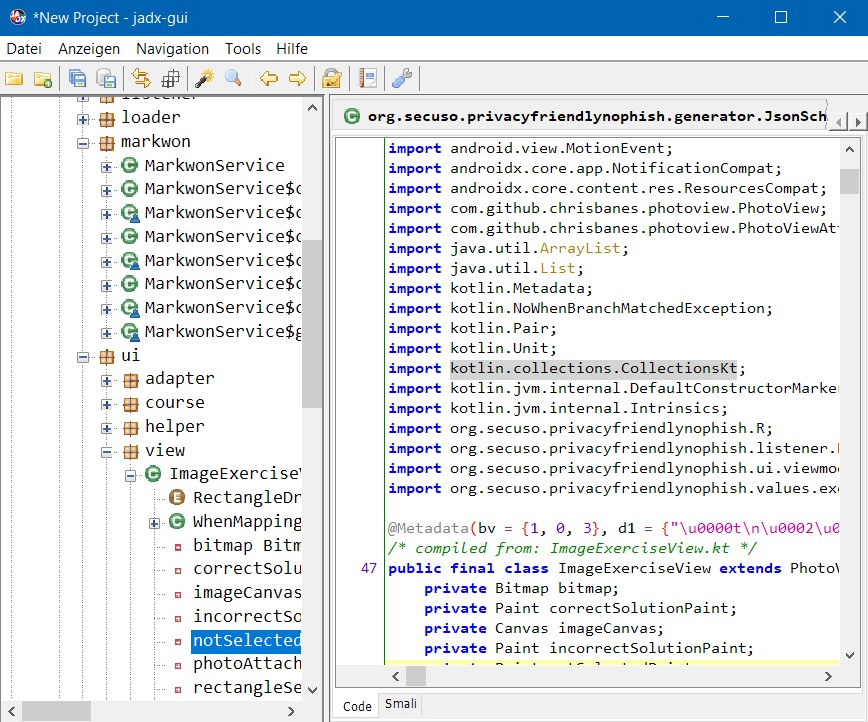
\includegraphics[width=\linewidth]{bilder/jadx.jpg}
    \caption{GUI-Oberfläche von JADX unter Windows 10} % nicht ins Glossar hinzufügen!
    \label{fig:jadx0}
\end{figure}

\section{Neuronale Netze}
In diesem Abschnitt werden die Grundlagen für die Entwicklung von neuronalen Netzen und Autoencodern erläutert.

\subsection{Neuronen und Schichten}
\label{subsec:activation}
Künstliche neuronale Netze sind eine Technologie des maschinellen Lernens. Diese werden laut Goodfellow et al.~\cite[S. 1-2]{goodfellowDeepLearningUmfassende2018} verwendet, um es Computern zu ermöglichen aus Erfahrungen zu lernen. Auf diese Weise können komplexe Konzepte erlernt werden, ohne dass ein Mensch das dafür notwendige Wissen formal beschreiben muss. Neuronale Netze extrahieren dabei Muster aus Rohdaten~\cite[S. 3]{goodfellowDeepLearningUmfassende2018}. An die Funktionsweise des menschlichen Gehirns angelehnt, funktionieren sie, indem künstliche Neuronen miteinander verbunden werden. Diese Neuronen gehen auf die Erfindung des \emph{Perzeptron} durch Rosenblatt~\cite{rosenblattPerceptronProbabilisticModel1958} im Jahr 1958 zurück. Ein solches Perzeptron wird in Abb.~\ref{fig:perceptron} dargestellt.

\begin{figure}[htbp]
    \centering
    \tikzstyle{line} = [draw, -latex']
    \begin{tikzpicture}[
        roundnode/.style={ellipse, draw=black, minimum height=15mm, minimum width=30mm, very thick},
        emptynode/.style={rectangle, very thick, minimum size=5mm},
        ]
        %Nodes
        \node[emptynode] (x1) {$x_1$};
        \node[emptynode] (x0) [above=of x1] {$x_0$};
        \node[emptynode] (x2) [below=of x1] {$x_2$};

        \node[roundnode] (sum) [right=of x1] {$\sum^n_{i=0} w_i * x_i$};
        \node[roundnode] (activation) [right=of sum] {$f(z)$};
        \node[emptynode] (o) [right=of activation] {$o$};
        %Lines
        \path [line] (x0) -- node [midway,above] {$w_0$} (sum);
        \path [line] (x1) -- node [midway,above] {$w_1$} (sum);
        \path [line] (x2) -- node [midway,above] {$w_2$} (sum);

        \path [line] (sum) -- node [midway,above] {$z$} (activation);
        \path [line] (activation) -- node [midway,above] {} (o);
    \end{tikzpicture}
    \caption{Beispielhafte Zusammensetzung eines Neurons mit drei Eingängen und einem Ausgang~\cite[S. 28]{kaulTheoreticalCharacterizationDeep2020}}
    \label{fig:perceptron}
\end{figure}

\pagebreak
Ein Neuron hat beliebig viele Eingänge $n \in \mathbb{N}$, aus welchen eine gewichtete Summe $z$ gebildet wird, die wie folgt definiert ist:

\begin{equation}
    z \coloneq s(x,w) = \sum_{i=0}^n w_i \cdot x_i
\end{equation}


Diese Summe $z$ wird als Eingabe für die sogenannte Aktivierungsfunktion $f(z)$ verwendet. Die Ausgabe der Aktivierungsfunktion ist die des gesamten Neurons. In der Forschungsgemeinschaft wird inzwischen eine Reihe an Aktivierungsfunktionen für die Entwicklung von Autoencodern verwendet. Davon ist die Sigmoid-Funktion eine der am häufigsten genutzten Funktionen. Sie ist eine logistische Funktion, welche sich wegen ihrem charakteristischen Wertebereich [0,1] besonders für neuronale Netze mit Ausgaben aus demselben Wertbereich eignet. Dies ist bei Bildinformationen der Fall, da hier aufgrund der einfacheren Handhabung üblicherweise der ganzzahlige Wertebereich $[0 \isep 255]$ auf das Intervall $[0,1]$ projiziert wird. Die Sigmoid-Funktion ist wie folgt definiert:

\begin{equation}
    \sigma (z) = \frac{1}{1+e^{-z}}
\end{equation}

Eine Funktion mit einem ähnlichen Funktionsgraphen ist der Tangens Hyperbolicus (tanh-Funktion). Dieser hat, anders als die Sigmoid-Funktion, den Wertebereich $[-1,1]$. Nach Goodfellow et al.~\cite[S. 215]{goodfellowDeepLearningUmfassende2018} leistet der Tangens Hyperbolicus normalerweise als Aktivierungsfunktion bessere Arbeit als die Sigmoid-Funktion. Der Tangens Hyperbolicus ist wie folgt definiert:

\begin{equation}
    tanh(z) = \frac{sinh(z)}{cosh(z)} = 1 - \frac{2}{e^{2z}+1}
\end{equation}

Die ReLU-Funktion ist eine sehr häufig genutzte Aktivierungsfunktion. Sie lässt sich sehr leicht optimieren, da ihre Gradienten sowohl groß als auch konsistent sind~\cite[S.~213]{goodfellowDeepLearningUmfassende2018}. Die Funktion entspricht der linearen Einheit im positiven Definitionsbereich und nimmt für $z=0$ und im negativen Definitionsbereich den Wert 0 an.

\begin{equation}
    relu(z) = max\{0, z\}
\end{equation}

\pagebreak
Zur ReLU-Funktion existieren mehrere Generalisierungen, welche ähnlich gut wie oder besser als die ReLU-Funktion funktionieren~\cite[S. 213]{goodfellowDeepLearningUmfassende2018}. In dieser Masterarbeit wird die sogenannte LeakyReLU-Funktion verwendet. Diese unterscheidet sich von der ReLU-Funktion darin, dass sie nicht den Wert 0 im negativen Definitionsbereich annimmt, sondern eine lineare Funktion mit beliebiger Steigung $\alpha$ darstellt. Oft und in dieser Masterarbeit gilt $\alpha = 0,01$. Die LeakyReLU-Funktion ist wie folgt definiert:

\begin{equation}
    leakyrelu(z) =
    \begin{cases}
        z & z > 0 \\
        \alpha z & sonst
    \end{cases}
\end{equation}

In dieser Arbeit werden die ReLU-, LeakyReLU-, Sigmoid- und die tanh-Funktion verwendet. In Abb.~\ref{fig:sigmoid} werden diese Funktionen dargestellt.



\begin{figure}
    \centering
\begin{tikzpicture}[declare function={sigma(\x)=1/(1+exp(-\x));
    sigmap(\x)=sigma(\x)*(1-sigma(\x));}]
    \begin{axis}%
    [
        xmin=-6,
        xmax=6,
        axis x line=bottom,
        ytick={0,.5,1},
        ymax=1,
        axis y line=middle,
        samples=100,
        domain=-6:6,
        legend style={at={(.4,0.9)}}
    ]
        \addplot[blue,mark=none]   (x,{sigma(x)});
        % \addplot[red,dotted,mark=none]   (x,{sigmap(x)});
        \legend{$\sigma(z)$}
    \end{axis}
\end{tikzpicture}
\begin{tikzpicture}[]
    \begin{axis}%
    [
        xmin=-6,
        xmax=6,
        axis x line=bottom,
        ytick={-1,-0.5,0,.5,1},
        ymax=1,
        axis y line=middle,
        samples=100,
        domain=-6:6,
        legend style={at={(.4,0.9)}}
    ]
        \addplot[blue,mark=none]   (x,{tanh(x)});
        % \addplot[red,dotted,mark=none]   (x,{sigmap(x)});
        \legend{$tanh(z)$}
    \end{axis}
\end{tikzpicture}
\begin{tikzpicture}
    \begin{axis}[
        domain=-8:8,
        axis x line=bottom,
        axis y line=middle,
        legend style={at={(.4,0.9)}}
        ]
        \addplot+[mark=none,blue,domain=-8:0] {0};
        \addplot+[mark=none,blue,domain=0:5] {x};
        \legend{$relu(z)$}
    \end{axis}
\end{tikzpicture}
\begin{tikzpicture}
    \begin{axis}[
        domain=-8:8,
        axis x line=middle,
        xtick={-8,-6,-4,-2,0,2,4},
        hide obscured x ticks=false,
        axis y line=middle,
        legend style={at={(.4,0.9)}}
        ]
        \addplot+[mark=none,blue,domain=-8:0] {0.01*x};
        \addplot+[mark=none,blue,domain=0:5] {x};
        \legend{$leakyrelu(z)$}
    \end{axis}
\end{tikzpicture}
\caption{Darstellungen der in dieser Arbeit genutzten Aktivierungsfunktionen (LeakyReLU-Funktion für $\alpha = 0,01$)}
\label{fig:sigmoid}
\end{figure}

In neuronalen Netzen werden Neuronen üblicherweise horizontal und vertikal angeordnet. Auf der horizontalen Ebene werden Netze üblicherweise in Schichten (engl. \emph{Layer}) gegliedert, die auf der vertikalen Ebene miteinander verbunden sind. Diese Schichten bilden zusammen ein neuronales Netz. Insbesondere auf dem Gebiet der Bild- und Sprachverarbeitung hat sich diese Technik durchgesetzt, sodass man oft von tiefen neuronalen Netzen spricht. Dies gilt auch im Kontext dieser Arbeit. Neuronale Netze lassen sich in zwei Gruppen einteilen: Netze, in denen die Verbindungen zwischen Schichten nur in eine Richtung verlaufen (sog. Feedforward-Netze) und \glspl{rnn}, in denen die Verbindungen in Schleifen verlaufen können, um zeitliche Abhängigkeiten abbilden zu können. Am \gls{fzi} werden sogenannte \glspl{ctrnn} erforscht, welche zu den \glspl{rnn} gehören. Mit Hilfe dieser \glspl{ctrnn} soll das automatisierte Testen von \gls{gui}-Oberflächen ermöglicht werden.

\subsection{Lernverfahren}
\label{subsec:lernverfahren}
\todo{Adamax beschreiben}
In dieser Arbeit werden neuronale Netze durch das Verfahren des Gradientenabstiegs mittels Backpropagation nach Rumelhart et al.~\cite{rumelhartLearningRepresentationsBackpropagating1986} trainiert. Dieser Algorithmus funktioniert durch Rückführung des Fehlers der Ausgabe durch das Netz. Daher ist es wichtig zu bestimmen, wie groß der Unterschied zwischen der aktuellen und der gewünschten Ausgabe des Netzes ist. Um dies zu berechnen, werden Fehlerfunktionen verwendet.

\subsubsection{Fehlerfunktionen}
\label{sec:errorfunction}

Die am weitesten verbreitete Fehlerfunktion ist die \glsentrylong{mse}~\cite[S. 15]{yeDeepDiveKeras2022}, die von der tatsächlichen Ausgabe des Netzes $y \in \mathbb{R}^n$ und dem Zielwert $t \in \mathbb{R}^n$ abhängig ist. Die Funktion ist wie folgt definiert:

\begin{equation}
    mse(y,t) = \frac{1}{n} \sum^n_{i=1}(y_i - t_i)^2
\end{equation}

Eine weitere, häufig verwendete Fehlerfunktion ist die \glsentrylong{bce}~\cite{hoRealWorldWeightCrossEntropyLoss2020}. Diese ist ebenfalls von der tatsächlichen Ausgabe des Netzes $y$ und dem Zielwert $t$ abhängig und ist wie folgt definiert:

\begin{equation}
    bce(y,t) = - \frac{1}{n} \sum^n_{i=1}[t_n \cdot \log y_n + (1-t_n) \cdot \log (1-y_n)]
\end{equation}

Die binäre Kreuzentropie ist als Fehlerfunktion beliebter als der \gls{mse}, da die Verwendung des \gls{mse} bei einigen Netzen sehr kleine Gradienten hervorrufen kann~\cite[S. 199]{goodfellowDeepLearningUmfassende2018}. Daher kommt diese Funktion auch zum Training der Netze dieser Arbeit zum Einsatz. Gleichzeitig ist der \gls{mse} als Fehlerfunktion sehr intuitiv und auch ohne tieferes Verständnis der Materie und Entropie durchschaubar. Um die Ausgaben von Netzen zu vergleichen, wird in dieser Arbeit der \gls{mse} verwendet.

\subsubsection{Algorithmus}

Mit dem Verfahren der Backpropagation ist es möglich, neuronale Netze mit mehreren Schichten zu trainieren. Dies funktioniert mittels eines Gradientenabstiegs und wird in Form von Pseudocode unter Algorithmus~\ref{algo:backprop} dargestellt. Hierzu wird eine Eingabe für das Netz vorwärts durch das Netz propagiert und eine Ausgabe berechnet. Diese Ausgabe wird mit der gewünschten Ausgabe verglichen und ein Fehler mittels der oben definierten Fehlerfunktion ermittelt. Das Ziel des Verfahrens ist deren Minimierung. Hierfür wird der ermittelte Fehler entsprechend den Gewichten der einzelnen Neuronen durch das Netz zurückpropagiert. Die Veränderung des Gewichts $\Delta w_{ij}$, wobei $w_{ij}$ das Gewicht des $i$-ten Eingangs des $j$-ten Neurons bezeichnet, berechnet sich wie folgt:

\begin{equation}
    \Delta w_{ij} = - \eta \frac{\partial E}{\partial w_{ij}}
\end{equation}

Hierbei bezeichnet $\eta$ die sogenannte Lernrate. Je größer die Lernrate ist, desto stärker werden die Gewichte $w_{ij}$ angepasst und desto schneller lernt das Netz. Eine zu große Lernrate kann jedoch dazu führen, dass das Netz nicht korrekt lernt. $\Delta w_{ij}$ wird in diesem Fall zu groß und verfehlt das Optimum der Fehlerfunktion, wodurch Instabilitäten entstehen~\cite[S.\,329]{goodfellowDeepLearningUmfassende2018}. Das neue Gewicht $w_{neu}$ berechnet sich dann folgendermaßen:

\begin{equation}
    w_{ij}^{neu} = w_{ij} + \Delta w_{ij}
\end{equation}

\IncMargin{1em}
\begin{algorithm}[htb]


    \KwIn{Eingabewerte $x \in \mathbb{R}^n$ mit Gewichten $w \in \mathbb{R}^{m \times n}$ und Lernrate $\eta \in \mathbb{R}$}
    \KwOut{Angepasster Gewichtsvektor $w_{neu}$}
    \BlankLine
    $z$ $\leftarrow$ 0\\
    \For{$i$ $\leftarrow$ $1$ \KwTo $m$ $\leftarrow$ $\#$ Schichten}{

    \For{$j$ $\leftarrow$ $1$ \KwTo $n$ $\leftarrow$ $\#$ Neuronen in Schicht}{
        \tcc{$f$ ist eine beliebige Aktivierungsfunktion}
        $p \leftarrow \# $ Nachfolger von $j$ in nächster Schicht \\
        $x_j \leftarrow f (\sum^p_{k=1} w_{jk}x_k)$
        % $z$ $\leftarrow$ $z$ + $w_{ij} \cdot x_{ij}$\;
    }
    }
    \BlankLine

    \For{$i$ $\leftarrow$ $1$ \KwTo $n$ $\leftarrow$ $\#$ Neuronen in Schicht}{
        \tcc{Berechne Ergebnis der Fehlerfunktion (Beispiel: \gls{bce})}
        $E(w) \leftarrow bce(x, t)$
    }
    \ForEach{$W$ $\in$ Lagen von Gewichten}{
        \ForEach{$w_{ji} \in W$}{
            $w_{ji} \leftarrow w^{neu}_{ji}$
        }
    }
    \Return{$w_{neu}$}
    \caption{Anpassung der Gewichte mit Backpropagation in einem neuronalen Netz. Hier wird zunächst die Ausgabe einer Schicht bestimmt und dann, mithilfe des Zielvektors, die neuen Gewichte im Netz. \cite[S. 316]{ertelNeuronaleNetze2021}}
    \label{algo:backprop}
\end{algorithm}
\DecMargin{1em}

\pagebreak

\subsubsection{Verwendung von Batches}
Für das Training von neuronalen Netzen werden Eingaben üblicherweise in sogenannte Batches (deutsch Stapel) gruppiert. Diese werden nacheinander durch das Netz propagiert und der Fehler berechnet. Die Gewichte werden erst zum Schluss aktualisiert.

\subsubsection{Optimierungsalgorithmen}
Die Lernrate ist nach Goodfellow et al.~\cite[S.~342]{goodfellowDeepLearningUmfassende2018} ein schwierig einzustellender Parameter. Um diese Auswahl automatisiert treffen zu können, haben sich sogenannte Optimierungsalgorithmen durchgesetzt, die für jeden Parameter eines Netzes eine eigene, dynamische Lernrate berechnen. Wie Goodfellow et al.~\cite[S.~347]{goodfellowDeepLearningUmfassende2018} beschreiben, wird der Optimierungsalgorithmus überwiegend auf Basis persönlicher Präferenzen gewählt. In dieser Arbeit kommt der Algorithmus Adamax zum Einsatz, der bereits in der Bachelorarbeit von Kies~\cite{kiesEntwicklungUndAnalyse2020} zum Einsatz kam. Adamax basiert auf dem Algorithmus Adam von Kingma und Ba~\cite{kingmaAdamMethodStochastic2017}, wobei die $L^\infty$-Norm statt der $L^2$-Norm zum Einsatz kommt.

\section{Convolutional Neural Networks}
\glspl{cnn} sind eine Spezialform der neuronalen Netze, die zur Verarbeitung von Daten mit einer bekannten rasterähnlichen Topologie eingesetzt werden~\cite[S. 369]{goodfellowDeepLearningUmfassende2018}. Bei diesen Netzen kommt die mathematische Operation der Faltung (engl. Convolution) zum Einsatz. Ein neuronales Netz ist ein \gls{cnn}, wenn in mindestens einer Schicht die Faltung als Operation eingesetzt wird~\cite[S. 369]{goodfellowDeepLearningUmfassende2018}.


\subsection{Faltung}
\label{subsec:convolution}


\begin{figure}[p]
    \centering
    \begin{tikzpicture}
        [
        default/.style={rectangle, draw=black, minimum height=7mm,  minimum width=7mm, very thick},
        decodernode/.style={rectangle, draw=green!60, fill=green!10, minimum height=5mm, very thick},
        bottlenecknode/.style={rectangle, draw=blue!60, fill=blue!60, minimum height=5mm, very thick},
        emptynode/.style={rectangle, very thick, minimum size=8mm},
        title/.style={font=\fontsize{6}{6}\color{black!50}\ttfamily},
      ]
      \tikzstyle{l} = [draw, -latex',thick]
        \node (a) [default] { $a$ };
        \node (b) [default, right=0.1cm of a] { $b$ };
        \node (c) [default, right=0.1cm of b] { $c$ };
        \node (d) [default, right=0.1cm of c] { $d$ };
        \node (e) [default, below=0.1cm of a] { $e$ };
        \node (f) [default, right=0.1cm of e] { $f$ };
        \node (g) [default, right=0.1cm of f] { $g$ };
        \node (h) [default, right=0.1cm of g] { $h$ };
        \node (i) [default, below=0.1cm of e] { $i$ };
        \node (j) [default, right=0.1cm of i] { $j$ };
        \node (k) [default, right=0.1cm of j] { $k$ };
        \node (l) [default, right=0.1cm of k] { $l$ };

        \node (w) [default, right=1cm of d] { $w$ };
        \node (x) [default, right=0.1cm of w] { $x$ };
        \node (y) [default, below=0.1cm of w] { $y$ };
        \node (z) [default, right=0.1cm of y] { $z$ };


        % \draw [draw=black!50] (dep.north west) rectangle ($(dep.north east) - (0, 2cm)$);
        \node (input) [draw=black, fit={(a) (b) (e) (f) }, very thick, inner sep=0.5mm] {};
        \node (filter) [draw=black, fit={(w) (x) (y) (z) }, very thick, inner sep=0.5mm] {};

        \node (label1) [emptynode, above=-0.2cm of input.north west, anchor=south west] { Eingabe };
        \node (label2) [emptynode, above=-0.2cm of filter.north west, anchor=south west] { Filter };

        \node (1) [default, align=left, minimum size=2cm, below=1cm of i] { $aw + bx + $\\ $ey + fz$ };
        \node (2) [default, align=left, minimum size=2cm, right=0.2cm of 1] { $bw + cx +$\\ $fy + gz$ };
        \node (3) [default, align=left, minimum size=2cm, right=0.2cm of 2] { $cw + dx +$\\ $gy + hz$ };
        \node (4) [default, align=left, minimum size=2cm, below=0.2cm of 1] { $ew + fx + $\\$iy + jz$ };
        \node (5) [default, align=left, minimum size=2cm, right=0.2cm of 4] { $fw+gx+$\\ $jy+kz$};
        \node (6) [default, align=left, minimum size=2cm, right=0.2cm of 5] { $gw+hx+$\\$ky+lz$ };

        \node (results) [draw=black, fit={(1)}, very thick, inner sep=1mm] {};
        \node (label3) [emptynode, above=-0.2cm of results.north west, anchor=south west] { Ausgabe };

        \draw [l] (input.west) -> ++(-1.5,0) node(upperleft){} |- (results.west);
        \draw [l] (filter.south) -> ++(0,-1.3) node(upperleft){} -- ++(-3.95,0) -- ++(0,-0.35);

      \end{tikzpicture}
    \caption{Beispiel einer Faltung. Dabei werden nur Fälle betrachtet, in denen der Filter vollständig im Bild liegt.~\cite{goodfellowDeepLearningUmfassende2018}}
    \label{fig:conv}
\end{figure}

\begin{figure}[p]
    \centering
    \resizebox*{\textwidth}{!}{\input{convolutional-layer.pdf_tex}}
    \caption{Darstellung der Faltungsoperationen in einer Convolutional-Schicht mit einer Eingabe bestehend aus $k$ Kanälen und $k'$ Filtern}
    \label{fig:conv_layer}
\end{figure}

Bei der Faltung werden im Kontext dieser Masterarbeit ausschließlich zweidimensionale Eingabedaten betrachtet, da es sich hier um Bildinformation handelt. Die Faltungsoperation benötigt zwei Matrizen als Eingabe. Im Fall von \glspl{cnn} ist dies die Eingabe des Netzes $I$ und der sog. Filter $K$ mit Dimension $m \times n$. Abb.~\ref{fig:conv} zeigt das Beispiel einer Faltung, in der die Faltungsoperation auf jeden Eintrag der Eingabe angewendet wird. Die Faltungsoperation ist wie folgt definiert~\cite[S. 371]{goodfellowDeepLearningUmfassende2018}:

\begin{equation}
    S(i,j) = (I * K)(i,j) = \sum_m \sum_n I(m,n) \cdot K(i-m, j-n)
\end{equation}


%Nach Goodfellow et al. wird die Faltung genutzt um und \emph{Parameter Sharing} umzusetzen. Bei Fully-Connected-Schichten wird zwischen den Schichten üblicherweise jedes Neuron einer Schicht mit jedem Neuron der Nachbarschichten verbunden, woraus eine hohe Anzahl an Parametern resultiert. Bei Convolutional-Schichten müssen nur die Parameter des Filters gespeichert werden, wodurch weitaus weniger Gewichte gespeichert werden müssen. Dies wird unter dem Begriff der \emph{spärlichen Interaktionen} zusammengefasst~\cite[S. 374]{goodfellowDeepLearningUmfassende2018}.


\subsection{Convolutional-Schicht}
\label{subsec:conv-layer}
Eine typische Convolutional-Schicht besteht üblicherweise aus drei Phasen. In der ersten Phase werden, wie im vorigen Abschnitt beschrieben, für jeden Eintrag der Eingabe Faltungen durchgeführt. Eine Schicht beinhaltet dabei $k$ Ausgangs-Kanäle, die jeweils einem Filter der Größe $m \times n$ entsprechen. Die Faltungsoperationen einer Schicht werden in Abb.~\ref{fig:conv_layer} dargestellt. Üblicherweise werden in der Literatur noch die Schrittweite $s$ (engl. \emph{Stride}) angegeben. Diese sagt aus, dass ein Filter nicht überall angewendet, sondern nur jede $s$-te Stelle der Ausgabe berechnet wird. Eine solche Schrittweite wird jedoch in dieser Masterarbeit nicht verwendet bzw. auf 1 gesetzt. Dementsprechend existieren pro Schicht $k \times m \times n$ Gewichte, die trainiert werden.
Die Ausgabe nach dieser Phase ist eine Matrix. Deren Dimension werden durch die Höhe $h$ und Breite $w$ der Eingabe, die Anzahl der Filter $k$ und deren Höhe $m$ und Breite $n$ wie folgt bestimmt:




\begin{displaymath}
    h - m + 1 \times w - n + 1 \times k
\end{displaymath}

Die zweite Phase besteht darin, die Ergebnisse der Faltungen als Eingabe für eine nichtlineare Aktivierungsfunktion (siehe Abschnitt~\ref{subsec:activation}) zu verwenden und die Ergebnisse zu berechnen. In der dritten Phase erfolgt üblicherweise ein sogenanntes Pooling. Hierzu existieren verschiedene Ansätze, von denen in dieser Masterarbeit das sog. Max-Pooling umgesetzt wurde. Dabei werden Bildbereiche einer bestimmten Größe (ähnlich dem Filter in Abschnitt~\ref{subsec:convolution}) zusammengefasst und durch den maximalen Wert in diesem Bereich ersetzt. Im Fall der in dieser Masterarbeit untersuchten Netze wird das Max-Pooling verwendet, um die Komplexität der Eingabe zu reduzieren und Information zu komprimieren.


\subsection{Übergang zwischen Schicht-Typen}
\label{subsec:flattening}
Die Ausgabe einer Convolutional-Schicht hat die Dimension $h \times w \times k$. Falls auf diese Schicht jedoch eine Fully-Connected-Schicht folgt, wird eine Eingabe der Dimension $1 \times (h \cdot w \cdot k)$ benötigt. Um dies zu erreichen findet ein sog. \emph{Flattening} statt. Dieses Flattening ignoriert die Dimension der Eingabe und überführt diese in eine Eingabe der gewünschten Dimension.

Falls die alten Dimensionen wiederhergestellt werden müssen, wird das \emph{Reshaping} durchgeführt, das die Eingabe wieder in die alte Dimension $h \times w \times k$ überführt.

\section{Autoencoder}
Autoencoder sind nach Ranzato et al. \cite{ranzatoUnsupervisedLearningInvariant2007} spezielle neuronale Netze, die aus drei Teilen bestehen: Ein Encoder, ein Decoder und ein Bottleneck (auch Repräsentation genannt). Alle Teile werden in Abb.~\ref{fig:autoencoder} dargestellt. Der Encoder sowie der Decoder sind in der Regel neuronale Netze, die von einem schmalen Feature-Vektor separiert werden, dem \emph{Bottleneck}. Das komplette Netz wird so trainiert, dass der Decoder die Eingabe rekonstruiert, \dh, dass die Ausgabe mit der Eingabe übereinstimmt. Da der Decoder nur Zugriff auf das Bottleneck hat und die Eingabe daraus rekonstruieren muss, erlernt der Encoder automatisch die Erstellung einer kodierten Repräsentation der Eingabe im Bottleneck. Da ein Autoencoder nur die Eingabe rekonstruieren muss und keine gelabelten Daten benötigt, zählt das Verfahren zu den unüberwachten Techniken.



Das Ziel der Verwendung eines Autoencoders ist in dieser Masterarbeit das automatische Erlernen einer komprimierten Kodierung von komplexen Daten. Die Qualität der Rekonstruktion ist hierbei abhängig von der Dimension des Bottlenecks. Ist dieses klein gewählt, kann die Eingabe unter Umständen nur unvollständig oder fehlerhaft wiederhergestellt werden.
Falls, wie in der vorliegenden Arbeit, nur eine effiziente Kodierung der Eingabe benötigt wird, kann der Encoder nach dem Training unabhängig vom Decoder verwendet werden.

\begin{figure}[h]
    \centering
    \tikzstyle{line} = [draw, -latex']
    \begin{tikzpicture}[
        encodernode/.style={rectangle, draw=red!60, fill=red!10, minimum height=5mm, very thick},
        decodernode/.style={rectangle, draw=green!60, fill=green!10, minimum height=5mm, very thick},
        bottlenecknode/.style={rectangle, draw=blue!60, fill=blue!60, minimum height=5mm, very thick},
        emptynode/.style={rectangle, very thick, minimum size=5mm},
        ]
        %Nodes
        \node[emptynode] (input) [minimum width=60mm]{Eingabe};
        \node[encodernode] (0) [below=0.2cm of input, minimum width=60mm]{};
        \node[encodernode] (1) [below=0.2cm of 0, minimum width=45mm] {};
        \node[encodernode] (2) [below=0.2cm of 1, minimum width=30mm] {};
        \node[bottlenecknode] (3) [below=0.2cm of 2, minimum width=15mm] {};
        \node[decodernode] (4) [below=0.2cm of 3, minimum width=30mm] {};
        \node[decodernode] (5) [below=0.2cm of 4, minimum width=45mm] {};
        \node[decodernode] (6) [below=0.2cm of 5, minimum width=60mm] {};
        \node[emptynode] (output) [below=0.2cm of 6, minimum width=60mm]{Rekonstruierte Eingabe};

        \node[emptynode] (encoder) [left=1.5cm of 1] {Encoder};
        \node[emptynode] (decoder) [left=1.5cm of 5] {Decoder};
        \node[emptynode] (dummy) [right=2.8cm of 5] {};
        \node[emptynode] (bottleneck) [right=.5cm of 3] {Bottleneck};
    \end{tikzpicture}
    \caption{Darstellung eines Autoencoders~\cite{alvernazAutoencoderaugmentedNeuroevolutionVisual2017}}
    \label{fig:autoencoder}
\end{figure}

Da ein Autoencoder symmetrisch aufgebaut ist, benötigt jede Schicht im Encoder ein Gegenstück im Decoder. Eine Fully-Connected-Schicht im Encoder, die $n$ Neuronen mit $m$ Neuronen verbindet, benötigt daher eine Schicht im Decoder-Teil, die $m$ Neuronen mit $n$ Neuronen verbindet. Ein einfacher, aus Fully-Connected-Schichten bestehender Autoencoder wird in Abb.~\ref{fig:autoencoder_net} dargestellt.


\begin{figure}[h]
    \centering
    \tikzstyle{line} = [draw, -latex']
    \begin{tikzpicture}[
        encodernode/.style={circle, draw=red!60, fill=red!10, minimum height=5mm, very thick},
        decodernode/.style={circle, draw=green!60, fill=green!10, minimum height=5mm, very thick},
        bottlenecknode/.style={circle, draw=blue!60, fill=blue!60, minimum height=5mm, very thick},
        emptynode/.style={rectangle, very thick, minimum size=5mm},
        ]
        %Nodes
        \node[encodernode] (00) {};
        \node[encodernode] [below= 0.3cm of 00] (01) {};
        \node[encodernode] [below= 0.3cm of 01] (02) {};
        \node[encodernode] [below= 0.3cm of 02] (03) {};
        \node[encodernode] [below= 0.3cm of 03] (04) {};
        \node[encodernode] [below= 0.3cm of 04] (05) {};
        \node[encodernode] [below= 0.3cm of 05] (06) {};
        \node[encodernode] [below= 0.3cm of 06] (07) {};
        \node[emptynode] [left= 1.9cm of 00] (x0) {};
        \node[emptynode] [left= 1.9cm of 01] (x1) {};
        \node[emptynode] [left= 1.9cm of 02] (x2) {};
        \node[emptynode] [left= 1.9cm of 03] (x3) {};
        \node[emptynode] [left= 1.9cm of 04] (x4) {};
        \node[emptynode] [left= 1.9cm of 05] (x5) {};
        \node[emptynode] [left= 1.9cm of 06] (x6) {};
        \node[emptynode] [left= 1.9cm of 07] (x7) {};

        \node[encodernode] [right= 1.9cm of 02] (10) {};
        \node[encodernode] [below= 0.3cm of 10] (11) {};
        \node[encodernode] [below= 0.3cm of 11] (12) {};
        \node[encodernode] [below= 0.3cm of 12] (13) {};

        \node[bottlenecknode] [right= 1.9cm of 11] (20) {};
        \node[bottlenecknode] [below= 0.3cm of 20] (21) {};

        \node[decodernode] [right= 1.9cm of 20] (31) {};
        \node[decodernode] [above= 0.3cm of 31] (30) {};
        \node[decodernode] [below= 0.3cm of 31] (32) {};
        \node[decodernode] [below= 0.3cm of 32] (33) {};

        \node[decodernode] [right= 1.9cm of 30] (42) {};
        \node[decodernode] [above= 0.3cm of 42] (41) {};
        \node[decodernode] [above= 0.3cm of 41] (40) {};
        \node[decodernode] [below= 0.3cm of 42] (43) {};
        \node[decodernode] [below= 0.3cm of 43] (44) {};
        \node[decodernode] [below= 0.3cm of 44] (45) {};
        \node[decodernode] [below= 0.3cm of 45] (46) {};
        \node[decodernode] [below= 0.3cm of 46] (47) {};
        \node[emptynode] [right= 1.9cm of 40] (y0) {};
        \node[emptynode] [right= 1.9cm of 41] (y1) {};
        \node[emptynode] [right= 1.9cm of 42] (y2) {};
        \node[emptynode] [right= 1.9cm of 43] (y3) {};
        \node[emptynode] [right= 1.9cm of 44] (y4) {};
        \node[emptynode] [right= 1.9cm of 45] (y5) {};
        \node[emptynode] [right= 1.9cm of 46] (y6) {};
        \node[emptynode] [right= 1.9cm of 47] (y7) {};

        \draw (00) -- (10);
        \draw (00) -- (11);
        \draw (00) -- (12);
        \draw (00) -- (13);
        \draw (01) -- (10);
        \draw (01) -- (11);
        \draw (01) -- (12);
        \draw (01) -- (13);
        \draw (02) -- (10);
        \draw (02) -- (11);
        \draw (02) -- (12);
        \draw (02) -- (13);
        \draw (03) -- (10);
        \draw (03) -- (11);
        \draw (03) -- (12);
        \draw (03) -- (13);
        \draw (04) -- (10);
        \draw (04) -- (11);
        \draw (04) -- (12);
        \draw (04) -- (13);
        \draw (05) -- (10);
        \draw (05) -- (11);
        \draw (05) -- (12);
        \draw (05) -- (13);
        \draw (06) -- (10);
        \draw (06) -- (11);
        \draw (06) -- (12);
        \draw (06) -- (13);
        \draw (07) -- (10);
        \draw (07) -- (11);
        \draw (07) -- (12);
        \draw (07) -- (13);

        \draw (10) -- (20);
        \draw (10) -- (21);
        \draw (11) -- (20);
        \draw (11) -- (21);
        \draw (12) -- (20);
        \draw (12) -- (21);
        \draw (13) -- (20);
        \draw (13) -- (21);

        \draw (20) -- (30);
        \draw (20) -- (31);
        \draw (20) -- (32);
        \draw (20) -- (33);
        \draw (21) -- (30);
        \draw (21) -- (31);
        \draw (21) -- (32);
        \draw (21) -- (33);

        \draw (30) -- (40);
        \draw (30) -- (41);
        \draw (30) -- (42);
        \draw (30) -- (43);
        \draw (30) -- (44);
        \draw (30) -- (45);
        \draw (30) -- (46);
        \draw (30) -- (47);
        \draw (31) -- (40);
        \draw (31) -- (41);
        \draw (31) -- (42);
        \draw (31) -- (43);
        \draw (31) -- (44);
        \draw (31) -- (45);
        \draw (31) -- (46);
        \draw (31) -- (47);
        \draw (32) -- (40);
        \draw (32) -- (41);
        \draw (32) -- (42);
        \draw (32) -- (43);
        \draw (32) -- (44);
        \draw (32) -- (45);
        \draw (32) -- (46);
        \draw (32) -- (47);
        \draw (33) -- (40);
        \draw (33) -- (41);
        \draw (33) -- (42);
        \draw (33) -- (43);
        \draw (33) -- (44);
        \draw (33) -- (45);
        \draw (33) -- (46);
        \draw (33) -- (47);

        \draw [-stealth] (x0) -- (00);
        \draw [-stealth] (x1) -- (01);
        \draw [-stealth] (x2) -- (02);
        \draw [-stealth] (x3) -- (03);
        \draw [-stealth] (x4) -- (04);
        \draw [-stealth] (x5) -- (05);
        \draw [-stealth] (x6) -- (06);
        \draw [-stealth] (x7) -- (07);
        \draw [-stealth] (40) -- (y0);
        \draw [-stealth] (41) -- (y1);
        \draw [-stealth] (42) -- (y2);
        \draw [-stealth] (43) -- (y3);
        \draw [-stealth] (44) -- (y4);
        \draw [-stealth] (45) -- (y5);
        \draw [-stealth] (46) -- (y6);
        \draw [-stealth] (47) -- (y7);
        %Lines
    \end{tikzpicture}
    \caption{Darstellung der Neuronen eines einfachen Autoencoders bestehend aus Fully-Connected-Schichten~\cite{alvernazAutoencoderaugmentedNeuroevolutionVisual2017}}
    \label{fig:autoencoder_net}
\end{figure}

\subsection{Convolutional Autoencoder}
Wenn ein Autoencoder Convolutional-Schichten enthält, spricht man von einem Convolutional Autoencoder, womit der Autoencoder auch zur Gruppe der \gls{cnn} gehört. Die Vorteile beim Einsatz von Convolutional-Schichten wurden in Abschnitt~\ref{subsec:conv-layer} beschrieben.

Ähnlich den Fully-Connected-Schichten, benötigen auch Convolutional-Schichten ein Gegenstück im Decoder, welche das Pooling und die Faltungsvorgänge umkehrt. Daher werden entsprechend Unpooling- und Transposed-Convolution-Phasen (deutsch etwa \emph{Transponierte-Faltungs-Phasen}) benötigt, um das Max-Pooling und die Faltung rückgängig zu machen.

% In dieser Masterarbeit wird nur das Max-Pooling umgesetzt, weshalb an dieser Stelle nur das Max-Unpooling erläutert wird. Das Max-Pooling ist nicht vollständig reversibel, da alle Werte außer dem Maximalwert verloren gehen. Das Max-Unpooling schreibt den Maximalwert an dessen ursprünglichen Index und setzt alle weiteren Werte auf 0. Der ursprüngliche Index des Maximalwertes muss nach dem Max-Pooling entsprechend gespeichert werden.

% Im Anschluss an das Unpooling folgt die transponierte Faltung. Dabei wird gedanklich die Faltung umgekehrt. Der Filter wird auf die Eingabe angewandt, wobei diesmal die Ergebnisse

% \begin{equation}
%     S(i,j) =
% \end{equation}

% \begin{figure}[htbp]
%     \centering
%     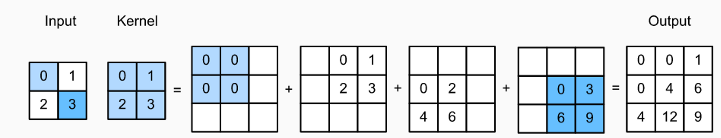
\includegraphics[width=\textwidth]{bilder/transposedconv.png}
%     \caption{Beispiel einer transponierten Faltung}
%     \label{img:transposed_conv}
% \end{figure}

\subsection{Variational Autoencoder}
Der \gls{vae} ist ein Ansatz, der 2014 durch Kingma und Welling~\cite{kingmaAutoEncodingVariationalBayes2014} vorgestellt wurde. Bei diesem Ansatz geht es darum, generative Ansätze mit konventionellen Autoencodern zu verbinden. Ein \gls{vae} unterscheidet sich gegenüber einem konventionellen Autoencoder in zwei Punkten. Zunächst wird am Bottleneck eine zusätzliche Schicht eingefügt, die die Werte im Bottleneck verändert. Darüber hinaus wird die Fehlerfunktion verändert, indem die sogenannte Kullback-Leibler-Divergenz addiert wird.

\subsubsection*{VAE-Schicht}
\label{subsubsec:vae-layer}
Nach dem Encoding-Vorgang wird die letzte Schicht des Encoders in zwei verschiedene Schichten aufgeteilt: die Schicht der Mittelwerte $\mu$ und die der Standardabweichung $\sigma$. Die Schicht der Standardabweichung wird dabei mit einem zufälligen Faktor $\epsilon$ multipliziert und auf die Schicht der Mittelwerte addiert, woraus sich die Werte des Bottlenecks $x$ ergeben. Damit ist $x$ wie folgt definiert:

\begin{equation}
    x = \mu + \epsilon \cdot \sigma
\end{equation}

Die Schichten $\mu$ und $\sigma$ werden im folgenden gemeinsam als \gls{vae}-Schicht bezeichnet und in Abb.~\ref{fig:vae-layer} dargestellt. Durch diesen Vorgang wird ein Rauschen hinzugefügt, durch welches ein Autoencoder die Normalverteilung lernen soll. Aus ähnlichen Werten am Bottleneck sollen ähnliche Ergebnisse resultieren. Das Lernen wird so kontinuierlich~\cite{yeVersatilityAutoencoders2022}.

\begin{figure}[p]
    \centering
    \tikzstyle{line} = [draw, -latex']
    \begin{tikzpicture}[
        encodernode/.style={rectangle, draw=red!60, fill=red!10, minimum height=5mm, very thick},
        decodernode/.style={rectangle, draw=green!60, fill=green!10, minimum height=5mm, very thick},
        bottlenecknode/.style={rectangle, draw=blue!60, minimum height=5mm, very thick},
        emptynode/.style={rectangle, very thick, minimum size=5mm},
        ]
        %Nodes
        \node[emptynode] (input) [minimum width=60mm]{Eingabe};
        \node[encodernode] (0) [below=0.5cm of input, minimum width=70.5mm]{};
        \node[encodernode] (1) [below=0.5cm of 0, minimum width=60.5mm] {};
        \node[encodernode] (2) [below=0.5cm of 1, minimum width=50.5mm] {};
        \node[emptynode] (bottleneck) [below=0.5cm of 2] {};
        \node[emptynode] (bottleneck2) [below=0.1cm of bottleneck] {};

        \node[bottlenecknode] (mu) [right=0.1cm of bottleneck, minimum width=40.5mm] {$\mu$};
        \node[bottlenecknode] (mu2) [below=0.1cm of mu, minimum width=7mm] {$\mu_2$};
        \node[bottlenecknode] (mu1) [left=0.1cm of mu2, minimum width=7mm] {$\mu_1$};
        \node[bottlenecknode] (mu0) [left=0.1cm of mu1, minimum width=7mm] {$\mu_0$};
        \node[bottlenecknode] (mu3) [right=0.1cm of mu2, minimum width=7mm] {$\mu_3$};
        \node[bottlenecknode] (mu4) [right=0.1cm of mu3, minimum width=7mm] {$\mu_4$};

        \node[bottlenecknode] (sigma) [left=0.1cm of bottleneck, minimum width=40.5mm] {$\sigma$};
        \node[bottlenecknode] (sigma2) [below=0.1cm of sigma, minimum width=7mm] {$\sigma_2$};
        \node[bottlenecknode] (sigma1) [left=0.1cm of sigma2, minimum width=7mm] {$\sigma_1$};
        \node[bottlenecknode] (sigma0) [left=0.1cm of sigma1, minimum width=7mm] {$\sigma_0$};
        \node[bottlenecknode] (sigma3) [right=0.1cm of sigma2, minimum width=7mm] {$\sigma_3$};
        \node[bottlenecknode] (sigma4) [right=0.1cm of sigma3, minimum width=7mm] {$\sigma_4$};


        \node[bottlenecknode] (x2) [below=1cm of bottleneck2, minimum width=7mm] {$x_2$};
        \node[bottlenecknode] (x1) [left=0.1cm of x2, minimum width=7mm] {$x_1$};
        \node[bottlenecknode] (x0) [left=0.1cm of x1, minimum width=7mm] {$x_0$};
        \node[bottlenecknode] (x3) [right=0.1cm of x2, minimum width=7mm] {$x_3$};
        \node[bottlenecknode] (x4) [right=0.1cm of x3, minimum width=7mm] {$x_4$};

        \node[bottlenecknode] (real_bottleneck) [below=0.1cm of x2, minimum width=40.5mm] {$x$};
        \node[emptynode] (representation) [left=1.0cm of real_bottleneck, yshift=0.29cm] {Kodierte Repräsentation};

        \node[decodernode] (4) [below=0.5cm of real_bottleneck, minimum width=50.5mm] {};
        \node[decodernode] (5) [below=0.5cm of 4, minimum width=60.5mm] {};
        \node[decodernode] (6) [below=0.5cm of 5, minimum width=70.5mm] {};
        \node[emptynode] (output) [below=0.5cm of 6, minimum width=60mm]{Rekonstruierte Eingabe};

        \draw [-stealth] (sigma0.south) -- (x0.north);
        \draw [-stealth] (sigma1.south) -- (x1.north);
        \draw [-stealth] (sigma2.south) -- (x2.north);
        \draw [-stealth] (sigma3.south) -- (x3.north);
        \draw [-stealth] (sigma4.south) -- (x4.north);
        \draw [-stealth] (mu0.south) -- (x0.north);
        \draw [-stealth] (mu1.south) -- (x1.north);
        \draw [-stealth] (mu2.south) -- (x2.north);
        \draw [-stealth] (mu3.south) -- (x3.north);
        \draw [-stealth] (mu4.south) -- (x4.north);

        \draw [-stealth] (2.south) -- (sigma.north);
        \draw [-stealth] (2.south) -- (mu.north);

        \draw [-stealth] (real_bottleneck.south) -- (4.north);
        \draw [-stealth] (4.south) -- (5.north);
        \draw [-stealth] (5.south) -- (6.north);
        \draw [-stealth] (0.south) -- (1.north);
        \draw [-stealth] (1.south) -- (2.north);


        \node[emptynode] (encoder) [left=2cm of 1, xshift=-0.77cm] {Encoder};
        \node[emptynode] (decoder) [left=2cm of 5, xshift=-0.7cm] {Decoder};
    \end{tikzpicture}
    \caption{Darstellung eines Autoencoders mit der Schicht der Mittelwerte und der Schicht der Standardabweichungen nach Ye~\cite{yeVersatilityAutoencoders2022}}
    \label{fig:vae-layer}
\end{figure}

\subsubsection*{Kullback-Leibler-Divergenz}
\label{subsubsec:kldiv}
Die Kullback-Leibler-Divergenz misst laut Ye~\cite[S. 180]{yeVersatilityAutoencoders2022} das Ausmaß der Divergenz zwischen zwei Verteilungsfunktionen. Bei Betrachtung der Autoencoder würde diese dafür benötigt, eine gleichmäßige und kontinuierliche Verteilung zu lernen und zu verhindern, dass mehrere Cluster entstehen. Die Kullback-Leibler-Divergenz wird dabei auf die Fehlerfunktion addiert und wird minimal, wenn der Mittelwert 0 und die Standardabweichung 1 beträgt. Damit wird das Netzwerk für Clustering und die Reduktion der Standardabweichung bestraft. Die Kullback-Leibler-Divergenz betrachtet zwei Wahrscheinlichkeitsverteilungen $P$ und $Q$ und ist wie folgt definiert~\cite[S. 80]{goodfellowDeepLearningUmfassende2018}:

\begin{equation}
    D_{KL} (P || Q) = \mathbb{E}_{X \sim P} [log \frac{P(x)}{Q(x)}]
\end{equation}

% \begin{itemize}
%     \item Zweck --> Dimensionen reduzieren
%     \item Funktionsweise --> symmetrisches NN
% \end{itemize}

\chapter{Verwandte Arbeiten}
Für die Bearbeitung der Masterarbeit existieren mehrere Vorarbeiten, die verwendet werden. Zunächst untersuchte bereits Annika Kies, inwiefern die \gls{gui}-Oberflächen von Computerspielen erlernt werden können \cite{kiesEntwicklungUndAnalyse2020}. In ihrer Bachelorarbeit untersuchte sie, ob neuronale Netze erlernen können, Computerspiele zu spielen. Hierfür entwickelte sie, ähnlich dem Ansatz dieser Masterarbeit, Autoencoder-Architekturen, um die Komplexität der Eingabedaten zu verringern. Kern ihrer Bachelorarbeit war es jedoch, Informationen aus der \gls{gui} über die derzeitige Spielsituation zu lernen, und nicht, \gls{gui}-Elemente zu erkennen. Beiden Arbeiten ist zwar gemein, dass jeweils wenige Pixel auf einem Bild besonders wichtig sein können, nichtsdestotrotz sind die wichtigen Elemente der \gls{gui} fundamental verschieden.

%Die beschriebene Problematik der unterschiedlichen Wichtigkeit von Pixeln ist ein Ergebnis ihrer Arbeit, sodass sie einige Handlungsempfehlungen gibt, wie beispielsweise dem unterschiedlichen Gewichten von Bildbereichen oder Pixeln. Diese können in dieser Masterarbeit weiter verfolgt und evaluiert werden.

Eine weitere Vorarbeit ist eine Dummy-Applikation\footnote{\url{https://github.com/neuroevolution-ai/MonkeyTestingDummyApp}, letzter Zugriff: 13.12.2021}, die im Rahmen eines Universitätspraktikums entstanden ist. Mit dieser Applikation wurden jedoch bisher keine Experimente durchgeführt, unter anderem, da diese in Python geschrieben ist und deshalb eine eher schlechte Ausführungsgeschwindigkeit aufweist. Die Applikation verfolgt auch ein anderes Ziel: die Anbindung der am Lehrstuhl entwickelten \gls{ctrnn} über einfachere Convolutional-Schichten.

Darüber hinaus existieren in der Forschungsgemeinschaft Ansätze, die Elemente des maschinellen Lernens verwenden, um \gls{gui}-Oberflächen zu testen.
Bauersfeld et al. \cite{bauersfeldUserInterfaceLevel} entwickelten einen Selektionsmechanismus, der auf dem von ihnen entwickelten \gls{gui}-Test-Framework \emph{TESTAR} \cite{bauersfeldGUITestJavaLibrary2012} aufsetzt. Im Gegensatz zu dieser Arbeit wird für die Erkennung von \gls{gui}-Elementen jedoch keine Bilderkennung verwendet, sondern die Accessibility API\footnote{\url{https://developer.apple.com/library/archive/documentation/Accessibility/Conceptual/AccessibilityMacOSX/}, letzter Zugriff: 13.12.2021} von macOS. Diese API ist in macOS-native Applikationen eingebaut und gibt auf Anfrage beliebige \gls{gui}-Elemente zurück. Unter macOS ist sie somit weit verbreitet, sodass keine Erkennung der \gls{gui}-Elemente benötigt wird. Die entsprechenden Lösungen sind jedoch auf macOS limitiert und können nicht auf andere Betriebssysteme oder Geräteklassen ausgeweitet werden. Wann welche Aktion durchführbar ist, muss des Weiteren auch durch den Tester definiert werden, womit ein entsprechender Zeitaufwand verbunden ist. Die durchführbaren Aktionen werden als Markov-Entscheidungsproblem modelliert, bevor Aktionen mit der Technik \emph{Q-Learning} generiert werden. Das Ziel hierbei ist eine \gls{gui} zu explorieren und dabei die Aktionen höher zu gewichten, die noch nicht ausgeführt wurden oder hinter denen sich Aktionen verbergen, die noch nicht ausgeführt wurden. Diese Berechnung wird durch eine Reward-Funktion durchgeführt.

AutoBlackTest \cite{marianiAutoBlackTestAutomaticBlackBox2012} liegt ein ähnlicher Ansatz zugrunde, der ebenfalls auf Q-Learning basiert. Hier können \gls{gui}-Oberflächen getestet werden, die durch den IBM Functional Tester\footnote{\url{https://www.ibm.com/docs/en/rft/10.0.2?topic=SSJMXE_10.0.2/com.ibm.rational.test.ft.ovrvw.doc/topics/c_test_app_dom_sup.html}, letzter Zugriff: 13.12.2021} unterstützt werden. Beide Ansätze unterscheiden sich von dem in dieser Masterarbeit vorgestellten Ansatz dahingehend, dass sie durch Technologien eingeschränkt sind.

%Darüber hinaus werden bei beiden Ansätzen die verwendeten Modelle während der Erkundung der \gls{gui} erstellt. Die hier verwendeten Autoencoder sowie die in Zukunft eingesetzten Netze werden jedoch vor dem Testvorgang trainiert. Durch das vorherige Training ist es daher möglich, dass diese daher zum Testzeitpunkt schnellere Ergebnisse erbringen können. Daneben könnte auch die Parallelisierbarkeit besser sein, da während dem Testvorgang keine Ergebnisse aus der Vergangenheit verwendet werden müssen. Stattdessen benötigt jeder Testvorgang nur die im Voraus trainierten, gleichen, Netze.

Daneben entwickelten Choi et al. \cite{choiGuidedGUITesting2013} den Ansatz \emph{Swift-Hand}, der aus dem Bereich des Active Learning stammt. Swift-Hand funktioniert ausschließlich mit Android-Apps und deren (nativen Schnittstellen). Der Ansatz funktioniert so, dass ein Modell einer \gls{gui} während dem Testen erstellt und exploriert wird, wobei durchgehend neue Zustände erstellt, aber auch vereinigt werden können. Auch dieser Ansatz unterscheidet sich vom vorliegenden darin, dass er nur für eine bestimmte Technologie (Android-Applikationen) geeignet ist.
% Genauso wird auch hier das Modell während der Ausführung der Tests dynamisch erstellt und nicht im Voraus.

Aus dem Bereich der suchbasierten Ansätze kommt EXSYST \cite{grossSearchbasedSystemTesting2012}. Hierbei kommen genetische Algorithmen zum Einsatz, in denen eine Population an Testsuiten mit Hilfe von Randomisierung (\emph{Mutation}) so verändert wird, dass sich ein Optimum durchsetzt. Auch EXSYST ist nicht technologieagnostisch, sondern unterstützt ausschließlich Java-Swing-Applikationen.

Alle hier vorgestellten Ansätze unterscheiden sich vom vorliegenden Ansatz dahingehend, dass diese sich auf den Teil beschränken, der durch die am \gls{fzi} entwickelten \gls{ctrnn} übernommen wird. Die Erkennung der \gls{gui}-Elemente, um die es in dieser Arbeit geht, wird von den beschriebenen Ansätzen nicht betrachtet, da dieser Vorgang durch Schnittstellen übernommen wird. Der hier vorgestellte Ansatz benötigt dagegen lediglich valide Ansichten der \gls{gui}.

%Ein Training gibt es hier nicht ebenso nicht, sodass die Optimierung zur Laufzeit stattfindet.

\todo{Vorarbeit: Visual Doom von Alvernaz und Togelius (siehe Arbeit von Annika)}

\chapter{Trainingsdatengenerator}
\label{cha:gui}
Der in dieser Arbeit gewählte Forschungsansatz beinhaltet die Verbesserung des Testens von \gls{gui}-Oberflächen durch Verwendung von Autoencodern. Um diese Autoencoder zu trainieren werden Daten über \gls{gui}-Oberflächen benötigt.

Der erste Schritt, der während der Bearbeitung durchgeführt wurde, ist daher die Entwicklung des Trainingsdatengenerators. Die Trainingsdaten werden hierbei prozedural generiert in Form von validen Ansichten von \glspl{gui}.
Um diesen Generator zu entwickeln wird eine \gls{gui} mit der Programmiersprache Rust als Mock-Applikation nachgebaut. In den nächsten Abschnitten werden daher die Hintergründe der Entscheidung für Rust und die hinter diesem Kapitel stehenden grundlegenden Fragen erläutert.
Darüber hinaus wird ein Framework zur \gls{gui}-Entwicklung benötigt. Im weiteren Verlauf dieses Kapitels werden die Anforderungen an diese Frameworks erklärt, verschiedene Frameworks evaluiert und eines davon zur Entwicklung ausgewählt. Im Anschluss folgt eine Beschreibung und Analyse der Entwicklung des Mocks und des Generators sowie ein Fazit.

Wie in Abschnitt \ref{sec:rust} beschrieben, ist der Grund für den Einsatz von Rust die Ausführungsgeschwindigkeit bei gleichzeitiger Speichersicherheit. Die Ausführungsgeschwindigkeit beeinflusst später die Trainingsgeschwindigkeit. Die Untersuchung der Einsetzbarkeit und der Reife der Sprache Rust und der Frameworks für anschließende Arbeiten ist, wie in Abschnitt \ref{sec:goal} beschrieben, ein sekundäres Ziel dieser Arbeit. Insbesondere ist angedacht, Rust bzw. solche Mocks für das Training der am \gls{fzi} entwickelten Netze zu verwenden. Daher werden in diesem Kapitel nicht nur die für diese Arbeit ausschlaggebenden Anforderungen, sondern darüber hinaus noch Weitere formuliert. Diese werden entsprechend auch zur Analyse und Bewertung der untersuchten Frameworks herangezogen.

Die \gls{gui}, die in dieser Masterarbeit nachgebaut werden soll, ist die des Dekompilierers JADX\footnote{\url{https://github.com/skylot/jadx}, letzter Zugriff: 13.12.2021}, der aus Android DEX\footnote{\url{https://source.android.com/devices/tech/dalvik/dex-format.html}, letzter Zugriff: 13.12.2021}- oder APK\footnote{\url{https://developer.android.com/guide/components/fundamentals}, letzter Zugriff: 13.12.2021}-Dateien Java-Quelltext generiert.
%Ein Screenshot dieser \gls{gui} wird in Abb.~\ref{fig:jadx} dargestellt.
Bei der Implementierung sollen möglichst alle Ansichten von JADX abgedeckt sein. JADX folgt den Betriebssystem-Designsprachen und verwendet viele native Elemente, die je nach Betriebssystem anders aussehen können. Um alle Varianten korrekt abzudecken müssten drei verschiedene Mocks bzw. ein Mock mit drei verschiedenen Designs entwickelt werden. Um diesen Aufwand zu reduzieren, erfolgt in dieser Masterarbeit die Umsetzung des Mocks auf Basis von JADX auf dem Betriebssystem Microsoft Windows 10 Version \mbox{10.0.19043}. Wie sich diese Autoencoder im Bezug auf die Designsprachen anderer Betriebssysteme verhalten, kann in weiteren Arbeiten analysiert werden.


% \begin{figure}
%     \centering
%     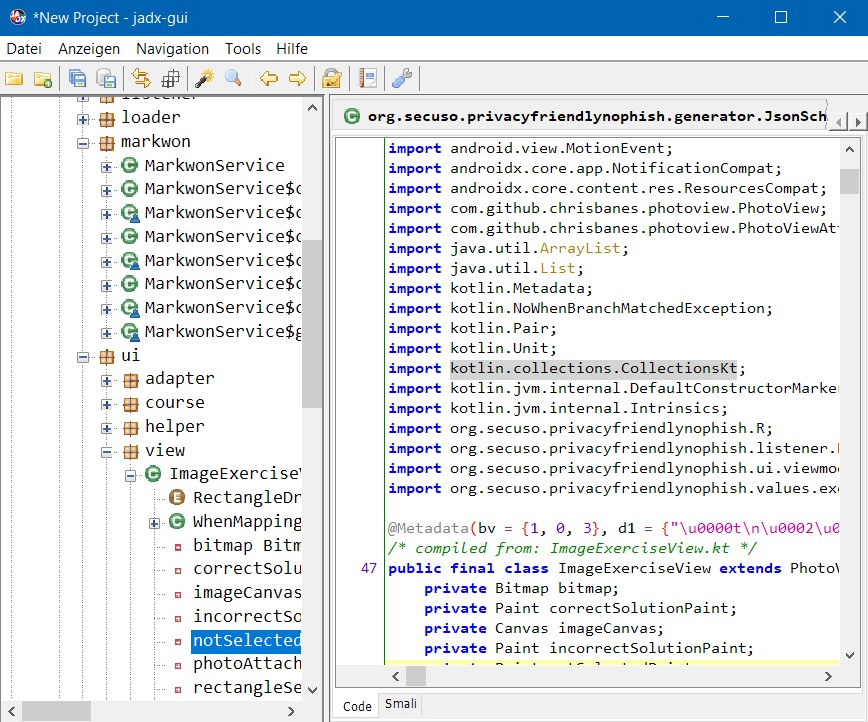
\includegraphics[width=\linewidth]{bilder/jadx.jpg}
%     \caption{GUI-Oberfläche von JADX unter Windows 10} % nicht ins Glossar hinzufügen!
%     \label{fig:jadx}
% \end{figure}


\section{Evaluierung von GUI-Frameworks}
\label{sec:gui-eval}
Nachdem das Vorbild des Mocks und die Gedanken hinter der Untersuchung in diesem Kapitel vorgestellt wurden, werden in diesem Abschnitt Anforderungen an die einzelnen Frameworks formuliert. Anschließend werden diese vorgestellt, dann grob sowie im Detail verglichen. Zum Schluss erfolgt die Auswahl des Frameworks und ein Fazit.

\subsection{Kriterien}
\label{subsec:criteria}
\todo{Aufteilen in Kriterien die gebraucht werden udn welche die erst später gebraucht werden --> Es soll ein Framework eingesetzt werden,
das sich möglichst auch schon für diese Einsatzzwecke eignet}

Eine Anforderung an Frameworks ist, dass diese auf möglichst jeder Desktop-Plattform laufen sollen. Insbesondere muss ein Framework unter Linux lauffähig sein, da der Server, der später den Mock ausführt, Linux verwendet. Darüber hinaus sollen möglichst alle Features in Rust implementiert sein. Einer der Hauptgründe Rust zu verwenden, sind die Vorteile bzgl. der Speichersicherheit. Viele Frameworks sind jedoch beispielsweise in C++ implementiert und werden lediglich über Bindings durch Rust-Applikationen verwendbar gemacht. Solche Frameworks können in Rust in der Regel nur unsicher aufgerufen werden, da C++ keine vergleichbaren Sicherheitsfeatures bietet.

Des Weiteren existieren einige Anforderungen, die nicht für diese Arbeit erfüllt sein müssen, aber in der Zukunft wichtig werden. Dazu gehört die Unterstützung von Offscreen Rendering durch die \gls{gui}-Frameworks. Eine Möglichkeit für Offscreen Rendering soll vorhanden sein, da die einzelnen Ansichten der \gls{gui} zukünftig auf einem Server ohne Verwendung von Betriebssystemfunktionen prozedural generiert werden sollen. Neben der Möglichkeit des Verzichts auf einen Fenstermanager und Betriebssystembibliotheken soll dadurch ein höherer Grad an Parallelisierung ohne Overhead erreicht werden. Bei Offscreen Rendering wird, vereinfacht beschrieben, nicht in ein Betriebssystemfenster (\dh auf den Bildschirm) gerendert. Stattdessen wird \zb im Fall von DirectX ein sog. Render Target~\cite{stevewhimsRenderTargetsOverview} gewählt, das eine Form einer Bitmap darstellt, die sich im Speicher befindet.
Offscreen Rendering ist für das Training der Autoencoder hilfreich. Da als Trainingsdaten lediglich Abbilder benötigt werden, ist es ausreichend, den Buffer (\dh die Bitmap) als Bilddatei abzuspeichern. So können Trainingsdaten ohne den Overhead bei der Initialisierung der Betriebssystem-Fenster generiert werden. Eine unbedingte Notwendigkeit für Offscreen Rendering besteht zum jetzigen Zeitpunkt jedoch nicht. Für die erhoffte Wiederverwendbarkeit im Zuge des Trainings der am \gls{fzi} entwickelten Netze wird Offscreen Rendering jedoch zur Voraussetzung. Hier soll ausschließlich auf der \gls{gpu} gerechnet werden, auf welcher keine Betriebssystemfunktionen zur Verfügung stehen.
Für das reine Generieren von Trainingsdaten ist diese Anforderung nicht notwendig. Die Trainingsdaten im Rahmen dieser Masterarbeit werden vorwiegend auf einem Desktop-PC generiert, auf welchem der Trainingsdatengenerator gestartet wird. Die benötigten Betriebssystemfunktionen stehen somit zur Verfügung.

Eine weitere Anforderung ist, dass das Framework möglichst ausschließlich die \gls{cpu} verwenden und nicht auf der \gls{gpu} rendern soll. Diese Anforderung ist für das reine Training der Autoencoder zunächst von untergeordneter Bedeutung, da hierfür ohne Probleme die \gls{gpu} verwendet werden kann. Da das Training der am \gls{fzi} entwickelten Netze jedoch auf der \gls{gpu} stattfinden soll, könnten Abhängigkeiten zu Grafikschnittstellen, welche zusätzliche \gls{gpu}-Zugriffe verursachen, für Komplikationen sorgen. Daneben ist es sinnvoll, dass die Generierung von Trainingsdaten auch ohne \gls{gpu} funktioniert, beispielsweise wenn diese schon durch andere Prozesse belegt ist. \gls{cpu}-Rendering ist im Vergleich zu Offscreen Rendering von geringerer Bedeutung, da das Nichtvorhandensein den zukünftigen Einsatz des Mocks nicht komplett verhindert, sondern unter Umständen nur die Nutzung der \gls{gpu} komplizierter wird. Des Weiteren könnten hier zukünftig Software-Implementierungen von Grafikschnittstellen wie lavapipe\footnote{\url{https://airlied.blogspot.com/2020/08/vallium-software-swrast-vulkan-layer-faq.html}, letzter Zugriff: 13.12.2021} Abhilfe schaffen. Mit lavapipe ist es möglich, Vulkan-Code ohne eine \gls{gpu} auszuführen. Dieser Ansatz ist jedoch vergleichsweise langsam und in einem frühen Stadium.

Zuletzt sollen die Frameworks möglichst schlank sein und keine Abhängigkeiten zu großen anderen Frameworks wie Qt\footnote{\url{https://www.qt.io/}, letzter Zugriff: 13.12.2021} oder GTK\footnote{\url{https://www.gtk.org/}, letzter Zugriff: 13.12.2021} aufweisen. Zusätzliche Abhängigkeiten erhöhen die Komplexität und verringern die Wahrscheinlichkeit, dass ein Einsatz ohne \gls{gpu}-Zugriffe möglich ist.


\subsection{GUI-Frameworks}

Als Basis für die Evaluierung der Frameworks dienen die Frameworks, die auf der Seite \emph{Are we GUI yet?}~\cite{AreWeGUI} aufgelistet sind. Sogenannte \emph{Are we\dots?}-Seiten werden im Rust-Umfeld traditionell dazu verwendet, den aktuellen Stand der Entwicklung zu einem spezifischen Thema zu darzulegen. Beispiele hierfür geben die Seiten \emph{Are we web yet?}\footnote{\url{https://www.arewewebyet.org}, letzter Zugriff: 13.12.2021} und \emph{Are we game yet?}\footnote{\url{https://arewegameyet.rs/}, letzter Zugriff: 13.12.2021}. Weitere, aktiv entwickelte Frameworks wurden in einer weiterführenden Recherche nicht gefunden. Diese Frameworks der Seite Are we GUI yet? werden in der Tabelle \ref{tab:frameworks} aufgelistet. Bei einigen Einträgen handelt es sich streng genommen um Bibliotheken und damit nicht um Frameworks. Im Unterschied zu Bibliotheken, geben Frameworks anhand von Schnittstellen und abstrakten Implementierungen Richtlinien für die Realisierung einer Lösung vor, welche eine bestimmte Architektur reflektieren~\cite[S.~412]{vogelArchitekturVorgehenWIE2009}. Dahingegen kann der Entwickler bei Verwendung einer Bibliothek selbst entscheiden, wann, wo und wie er diese einsetzt. Da Frameworks jedoch die Mehrheit darstellen und es sich bei den in Frage kommenden Einträgen ausschließlich um Frameworks handelt, wird hier zur besseren Lesbarkeit ausschließlich der Begriff \emph{Framework} verwendet.

In der Tabelle fehlt lediglich der Rust Qt Binding Generator, da dieser Bindings generiert um Rust-Quelltext in Qt aufrufbar zu machen. Damit ist diese Bibliothek nicht zur \gls{gui}-Entwicklung in Rust geeignet und wird daher hier nicht betrachtet. Bezüglich des Stands der Entwicklung der Bibliotheken und Frameworks werden in der Tabelle, soweit möglich, die Angaben des Entwicklers verwendet. Sofern der Entwickler selbst keine Angaben macht, wurden die Einträge als \emph{stabil} klassifiziert, falls die Versionsnummer mindestens 1.0 beträgt und in den anderen Fällen als \emph{instabil} klassifiziert. Azul wurde als \emph{sehr instabil} eingestuft, da hier nur Nightly Builds existieren und damit kein stabilisierter (Alpha- oder Beta-) Release.
Die mittlere Spalte der Tabelle enthält die wichtigsten grundlegenden Werkzeuge, Schnittstellen etc. auf denen das entsprechende Framework basiert. Dazu gehören verwendete Renderer (Raqote, GFX etc.), Grafikschnittstellen (wie OpenGL, Vulkan, DirectX etc.) bzw. deren Wrapper (Glium, wgpu etc.) oder GUI-Frameworks (Qt, GTK etc.). In der Spalte \emph{Anmerkung} befinden sich Anmerkungen zu den GUI-Frameworks sowie besondere Einschränkungen. Die Angabe \emph{Desktop} in der rechten Spalte ist hierbei eine Verallgemeinerung der Plattformen Windows, macOS und Linux/Unix. Diese Bezeichnung wurde gewählt, sofern alle drei Plattformen durch die Entwickler adressiert wurden. Die meisten Frameworks sind nicht in einer stabilen Version vorhanden und die unterstützten Plattformen und Schnittstellen können sich schnell ändern. Als Stichtag für die grobe Evaluierung wurde deshalb der 30.06.2021 gewählt. An diesem Tag musste die Vorauswahl der Frameworks getroffen werden, um genügend Zeit für die Einzelevaluierung und die Erstellung des Trainingsdatengenerators zu haben. Daher sind alle Informationen über Frameworks in diesem Kapitel auf dem Stand dieses Stichtages, um die Entscheidungsgrundlage darzulegen.


\subsection{Vorauswahl}

Die in Tabelle~\ref{tab:frameworks} dargestellten Informationen über die Frameworks lassen eine Vorselektion zu, in der viele Frameworks schon ausgeschlossen werden konnten. Zunächst sind offensichtlicherweise alle Frameworks nicht verwendbar, die den Desktop als Plattform nicht unterstützen. macOS oder Windows reichen hier nicht aus, da der entsprechende Server unter Linux läuft. Demnach entfallen auch eingebettete Plattformen oder das Web als Plattform. Darüber hinaus können auch die beschriebenen, nur in Form von Bindings für Rust bereitstehenden Frameworks aussortiert werden. Frameworks, die Qt oder GTK einsetzen, wurden ebenso aussortiert, da diese kein Offscreen Rendering
%\textcolor{red}{(jedenfalls ist dem Autor nichts bekannt - Quelle?)}
unterstützen, viele Abhängigkeiten haben und sehr groß sind. Nach dieser einfachen Vorselektion bleiben folgende Frameworks übrig: Azul, Conrod, Druid, egui, Iced, KAS und OrbTK.

Azul ist in einem sehr frühen Entwicklungsstadium ohne stabilisierter Release und wurde deshalb im weiteren Verlauf nicht berücksichtigt. Bei der Entwicklung von Druid ist es laut den Entwicklern kein Ziel, in eine benutzerdefinierte Render-Pipeline eingebettet zu werden~\cite{LinebenderDruid2018}. Druid unterstützt Offscreen Rendering aktuell nicht und es ist daher auch unwahrscheinlich, dass dies in Zukunft der Fall sein wird. Zukünftig wird genau dies jedoch benötigt, weshalb Druid ebenso nicht weiter berücksichtigt wurde.

Von den verbleibenden Frameworks verwendet ausschließlich OrbTK \gls{cpu}-Rendering mit der Bibliothek \emph{raqote}\footnote{\url{https://github.com/jrmuizel/raqote}, letzter Zugriff: 13.12.2021}. Die Frameworks Iced und KAS verwenden wgpu\footnote{\url{https://wgpu.rs/}, letzter Zugriff: 13.12.2021}, das eine Abstraktionsschicht für native Grafikschnittstellen wie Vulkan, Metal oder DirectX darstellt. Conrod oder egui bieten mehrere Backends an. Bei diesen kann es sich um Wrapper für Grafikschnittstellen, etwa in Form von Glium\footnote{\url{https://github.com/glium/glium}, letzter Zugriff: 13.12.2021} für OpenGL oder Vulkano\footnote{\url{https://github.com/vulkano-rs/vulkano}, letzter Zugriff: 13.12.2021} für Vulkan, oder um Grafik-Engines, \gls{gpu}-Rendering-Bibliotheken etc. handeln. Wie in Abschnitt~\ref{subsec:criteria} beschrieben wurde, ist \gls{cpu}-Rendering keine Anforderung, die auf jeden Fall erfüllt sein muss, da verschiedene Maßnahmen denkbar sind um das dort beschriebene Problem zu umgehen. \gls{gpu}-Rendering-Frameworks wurden daher vorerst weiter mit einbezogen.

\renewcommand{\tabularxcolumn}[1]{>{\raggedright\arraybackslash}p{#1}}
\newcolumntype{s}{>{\hsize=.84\hsize}X}
% \newcolumntype{l}{>{\hsize=.8\hsize}X}

% \begin{table}[htbp!]
%     \begin{center}
%         \caption{Klassifikationsergebnisse Kategorie \glqq Eingabedaten\grqq}
%         \bigskip

        \pgfplotstabletypeset[
            reset styles,
            debug=true,
            string type,
            header=false,
            col sep=semicolon,
            row sep=newline,
            column type=,
            skip first n=1,
            begin table={
              \begingroup\renewcommand{\arraystretch}{1.5}
              \begin{xltabular}{\textwidth}{XXXXXX}
                \caption{Untersuchte GUI-Bibliotheken und -Frameworks (Stand: 30.06.2021)} \label{tab:frameworks} \\
              \toprule
              \textbf{Name} & \textbf{Stand} & \textbf{Renderer / basiert auf / Schnittstelle} & \textbf{Anmerkung} & \textbf{Plattform} \\
              \midrule
              \endhead
            },
            end table={\bottomrule \end{xltabular}\endgroup},
            every head row/.style={ output empty row },  % suppress printing head row (numbers)
            % every head row/.style={after row=\midrule},
            % display columns/0/.style={string type,column name={\textbf{Name}}
            % },
            % display columns/1/.style={string type,column name={\textbf{Stand}}},
            % display columns/2/.style={string type,column name={\textbf{Renderer / basiert auf / Schnittstelle}}},
            % display columns/3/.style={string type,column name={\textbf{Anmerkung}}},
            % display columns/4/.style={string type,column name={\textbf{Plattform}}},
          ]{tabellen/FrameworksTabelle.csv}
%         \label{table1}
%     \end{center}
% \end{table}



\subsection{Detailvergleich}

Die verbleibenden Frameworks wurden detaillierter untersucht und gegebenenfalls Tests unterzogen. %Hier ist es nicht mehr möglich, eine Entscheidung ausschließlich anhand harter Kriterien zu treffen.
Die in Abschnitt \ref{sec:gui-eval} beschriebenen Kriterien werden von allen Frameworks außer OrbTK gleichermaßen erfüllt bzw. im Fall des \gls{cpu}-Renderings nicht erfüllt.
Weitere Entscheidungskriterien sind nun beispielsweise die Qualität der Dokumentation, die Entwicklungsaktivität, Kommunikationsmöglichkeiten mit den Entwicklern sowie die Unterstützung oder Verwendung möglichst etablierter Bibliotheken und Schnittstellen. Gute Kommunikationsmöglichkeiten mit den Entwicklern sind in diesem Fall besonders wichtig, da sich viele Frameworks noch in einem frühen Stadium befinden, in welchem die Dokumentation oft nur unvollständig vorhanden ist. Des Weiteren ist Offscreen Rendering kein zentrales Feature der meisten Frameworks und daher in der Regel nicht oder nur schlecht dokumentiert. Eine Übersicht der Entscheidungsgrundlage wird in Tabelle~\ref{table:frameworks_detail} dargestellt.


\begin{table}[htbp]
    \begin{center}

\rotatebox{90}{%
  \begin{minipage}{.85\textheight}
    \captionof{table}{Bewertung von GUI-Frameworks anhand weicher Kriterien}
    \label{table:frameworks_detail}
        \renewcommand{\arraystretch}{1.5}

        \begin{tabularx}{\textwidth}{ XXXXX }
            \toprule
            OrbTK & Iced  & KAS   & egui & Conrod \\
            \hline
            ++ \gls{cpu}-Rendering & + wgpu-Unterstützung & + wgpu-Unterstützung & + viele unterstützte Grafik-Backends, wgpu nur über 3rd-Party & + viele unterstützte Grafik-Backends \\
            + Entwicklerchat & + größte Entwicklergemeinschaft & + starke Entwicklertätigkeit & + starke Entwicklertätigkeit und mehrere Entwickler     & + starke Entwicklertätigkeit \\
            + Dokumentation durch Readmes, Chat, Beispiele und Rust Docs & + Entwicklerchat & - nur ein Hauptentwickler & + Diskussionsräume & o Anfänge eines Handbuchs, sonst nur Rust Docs \\
            - Geringer Entwicklungsfortschritt & + Dokumentation durch Readmes, Chat, Beispiele und Rust Docs & - Wenig Dokumentation abseits Beispiele & + Dokumentation durch Get Started, Diskussionen und Rust Docs & - Keine Beispiele \\
            - Nur ein Hauptentwickler & - etwas weniger Entwicklung in letzter Zeit & - leere Diskussionsräume & o Immediate Mode Toolkit & - kein Chat / Forum \\

            \bottomrule
        \end{tabularx}

\end{minipage}
}
\end{center}
\end{table}

\subsubsection*{Frameworks mit \gls{gpu}-Rendering}

Vor einer Beschreibung der einzelnen Frameworks ist es wichtig, die Bibliothek \mbox{wgpu} vorzustellen, welche in mehreren Frameworks verwendet wird. wgpu~\cite{GfxrsWgpu2018} ist eine Rust-native WebGPU\footnote{\url{https://www.w3.org/TR/webgpu/}, letzter Zugriff: 13.12.2021}-Implementierung, welche sich durch eine aktive Community auszeichnet. Die Entwicklung wird als Bestandteil von Firefox~\cite{GpuwebGpuwebImplementation2017} u.\,a. durch Mitarbeiter von Mozilla getragen~\cite{GfxrsWgpuPulse2018}, wobei WebGPU als Standard voraussichtlich durch das World Wide Web Consortium\footnote{\url{https://www.w3.org/}, letzter Zugriff: 13.12.2021} anerkannt wird~\cite{WebGPU}. Darüber hinaus unterstützt wgpu mehrere Grafikschnittstellen. Durch eine größere Anzahl an unterstützten Schnittstellen ist es wahrscheinlicher, dass für eine Schnittstelle eine reine Software-Implementierung existiert, welche eingesetzt werden kann. Ein Beispiel dafür ist lavapipe für Vulkan, wie in Abschnitt~\ref{subsec:criteria} beschrieben wurde.

\textbf{Iced~\cite{ramonHecrjIced2019}} ist ein \gls{gui}-Framework, das durch die \gls{gui}-Beschreibungssprache Elm\footnote{\url{https://elm-lang.org/}, letzter Zugriff: 13.12.2021} inspiriert ist. Iced legt laut eigenen Angaben einen Fokus auf Einfachheit und Typsicherheit und basiert auf der Bibliothek wgpu. Es existiert mit 12.100 Sternen auf Github, Commits von 89 verschiedenen Autoren \cite{ramonHecrjIced2019} und einem sehr aktiven Entwicklerchat \cite{IcedZulip} eine vergleichsweise große Entwicklergemeinschaft. Über den Chat können Fragen zur Nutzung geklärt werden, Diskussionen über die Weiterentwicklung stattfinden und Bugreports eingestellt werden.

\textbf{KAS~\cite{KasguiKas2019}} hat gegenüber Iced mit nur zwei Autoren eine deutlich kleinere Entwicklergemeinschaft und wesentlich weniger Dokumentation.
Das Framework ist durch Qt\footnote{\url{https://www.qt.io/}, letzter Zugriff: 13.12.2021} inspiriert und fokussiert sich nach eigenen Angaben auf Typsicherheit und eine schnelle, effiziente und responsive Benutzerschnittstelle. KAS unterstützt ebenfalls wgpu.

\textbf{egui~\cite{ernerfeldtEmilkEgui2019}} wird von den Autoren als Immediate Mode Toolkit bezeichnet, welche laut eigener Aussage die Eigenschaft haben, besonders einfach und unkompliziert zu sein, jedoch nur eingeschränkte Layout-Möglichkeiten bieten. egui zielt darauf ab, die am einfachsten zu benutzende \gls{gui}-Bibliothek zu sein und unterstützt eine große Anzahl an Integrationen (Web, Glium\footnote{\label{footn:glium}\url{https://github.com/glium/glium}, letzter Zugriff: 13.12.2021}, Bevy Game Engine\footnote{\url{https://bevyengine.org/}, letzter Zugriff: 13.12.2021}, Vulkano\footnote{\label{footn:vulkano}\url{https://github.com/vulkano-rs/vulkano}, letzter Zugriff: 13.12.2021},\dots). Vor dem Hintergrund, dass auch komplexere GUIs durch den Mock dargestellt werden sollen, könnte diese Eigenschaft in Zukunft zu Limitierungen führen.

\textbf{Conrod~\cite{PistonDevelopersConrod2014}} kombiniert laut eigener Aussage die Vorteile von Immediate Mode Toolkits mit denen klassischer \gls{gui}-Frameworks. Es bietet Unterstützung für GFX\footnote{\url{https://github.com/gfx-rs/gfx}, letzter Zugriff: 13.12.2021}, Glium\footnoteref{footn:glium}, OpenGl und Vulkano\footnoteref{footn:vulkano}. Conrod ist sehr unvollständig dokumentiert, da außer einer kurzen Anleitung, bei dem die meisten Kapitel noch nicht umgesetzt wurden, und Rust Docs keine Dokumentation existiert. Darüber hinaus existiert bei Conrod keine schnelle Kommunikationsmöglichkeit mit den Entwicklern oder anderen Nutzern.

\todo{Vor Abgabe: Angaben zu Frameworks checken! (insbesondere unterstützte Schnittstellen, etc.)}

\subsubsection*{Framework mit CPU-Rendering}
%\todo{Viel von dieser Info in nächstes Kapitel schieben}
\textbf{OrbTK} ist ein Framework, das zum Ziel hat, skalierbare Benutzerschnittstellen zu ermöglichen. Es basiert auf dem Entity-Component-System-Entwurfsmuster, welches aus der Videospielentwicklung stammt~\cite{muratetAccessibilitySeriousGames2020}, und verwendet Elemente des funktionalen sowie des reaktiven Programmierens \cite{RedoxosOrbtk2015}. Das Framework bietet den Vorteil, dass nur auf der \gls{cpu} gerendert wird und daher keine Abhängigkeiten zur Hardware bestehen. Eigene Tests mit OrbTK und Rücksprachen mit dem Entwickler~\cite{blasiusMomentItIt,blasiusHiDifficultSay} brachten das Ergebnis hervor, dass es zum aktuellen Zeitpunkt jedoch nicht möglich ist in einen Framebuffer ohne die Erstellung eines Fensters durch das Betriebssystem zu rendern. Aktuell würde jedoch der Quelltext überarbeitet und einige Komponenten entkoppelt, sodass dies in Zukunft möglich sei. Der gesteckte Zeitrahmen von mehreren Wochen bis Monaten ist dabei für eine produktive Verwendung im Rahmen dieser Masterarbeit zu lang. Dieser lange Zeitraum kommt durch die im Juli/August 2021 eher langsam verlaufende Entwicklung zustande~\cite{blasiusHiDifficultSay}. Zu diesem Zeitpunkt trug nur ein Entwickler in größerem Maß zum Projekt bei. Wie in Abschnitt~\ref{sec:gui-eval} beschrieben, ist Offscreen Rendering jedoch nicht allein ausschlaggebend für oder gegen eine Verwendung eines Frameworks, da die Trainingsdaten auch ohne dieses Feature generiert werden können.

Die Einarbeitungszeit bei OrbTK war kurz. Widgets, die Blöcke, aus denen eine \gls{gui} gebaut wird, können einfach komponiert und per Builder-Entwurfsmuster konfiguriert werden~\cite{RedoxosOrbtk2015}. Die Arbeit mit OrbTK war zu Beginn durch eine sehr schlechte Performance im Vergleich zu anderen Frameworks geprägt. Bereits bei einfachen Anwendungen kam es zu um mehrere Sekunden verzögerte Reaktionen auf Eingaben durch den Benutzer. Dieses Problem konnte jedoch dadurch behoben werden, dass das Release-Profil von Rust ausgewählt wurde. Bei diesem Profil verzichtet Rust auf viele Überprüfungen und führt Optimierungen durch~\cite{CustomizingBuildsRelease}. Eine Erklärungsmöglichkeit hierfür ist, dass bei OrbTK auch das Rendering durch Rust-Bibliotheken durchgeführt wird und nicht durch Grafikschnittstellen übernommen wird. Dadurch wird der Quelltext, welcher das Rendering durchführt, im Gegensatz zu anderen Frameworks erst durch das Release-Profil optimiert und ist nicht bereits voroptimiert. Overlays und zusätzliche Fenster sind mit OrbTK einfach umzusetzen.

\subsubsection*{Entscheidung}

Unter den Frameworks, die eine \gls{gpu} benötigen, ist Iced das vielversprechendste. Erste Tests mit Iced, in welchen das Menü und die Werkzeugleiste von JADX nachgebaut wurden, bestätigten dies. Die Einarbeitungszeit war verhältnismäßig gering und alle verbleibenden offenen Fragen konnten schnell im Entwicklerchat geklärt werden. Das Layout-System sowie die Erstellung von Komponenten funktionierte zuverlässig.

Bestimmte Funktionalitäten wie Overlays oder zusätzliche Betriebssystemfenster sind zum aktuellen Zeitpunkt nur unvollständig bzw. nicht umgesetzt.
Eine weitere Limitierung ist, dass Iced zunächst eine \gls{gpu} benötigt. Die verwendete Bibliothek wgpu setzt auf Vulkan und Metal -- eine Umsetzung für DirectX ist geplant~\cite{GfxrsWgpu2018}. Die am weitesten verbreiteten Implementierungen dieser Grafikschnittstellen benötigen zwar eine \gls{gpu}, eine rein \gls{cpu}-basierte Implementierung ist jedoch denkbar.

OrbTK ist durch das \gls{cpu}-Rendering in Zukunft unkompliziert durch das FZI zu verwenden. Da außerdem Features wie zusätzliche Fenster und Overlays existieren und trotz der recht kleinen Entwicklergemeinschaft fiel die Entscheidung auf OrbTK.





\section{Implementierung des Mocks}
\label{sec:impl}
Der Mock wurde unter Einsatz des Frameworks \emph{OrbTK} implementiert. Da die prozedurale Generierung, und damit die Variabilität, erst in späteren Schritten entwickelt wird, wurde in diesem Schritt JADX mit so wenigen Veränderungen wie möglich abgebildet. In diesem Abschnitt sollen das Ziel des Mocks und die Vor- und Nachteile der Entwicklung mit OrbTK erläutert werden, bevor die Eigenschaften und Limitierungen der Implementierung beschrieben werden.

\subsection{Ziel des Mocks}
\label{subsec:goal_mock}
Das Ziel hinter der Entwicklung dieses Mocks ist es, eine Datenquelle zu schaffen, die zum Training von Autoencodern verwendet werden kann. Diese Datenquelle soll aus validen Abbildern von \gls{gui}-Oberflächen bestehen und sich an der Anwendung JADX orientieren. Dabei geht es vorwiegend darum, real aussehende \glspl{gui} zu erstellen um herauszufinden, ob und wie \gls{gui}-Oberflächen von Autoencodern enkodiert werden können. Eine exakte Nachbildung von JADX ist daher nicht nötig und aus Gründen des Zeitaufwandes auch nicht sinnvoll. Es wird allein deshalb zu Abweichungen kommen, da OrbTK sich nicht an der Windows-Designsprache oder dem Design von JADX orientiert.

Eine sekundär zu beantwortende Frage ist, wie gut die Autoencoder noch mit der realen \gls{gui} von JADX funktionieren. In Kapitel \ref{cha:autoencoder} wird daher untersucht, inwiefern die Abweichungen zwischen Mock und realer \gls{gui} einen Effekt auf die Ergebnisse der Autoencoder haben.

Die Implementierung dieses Mocks wird in dieser Arbeit außerdem so beschränkt, dass nur \gls{gui}-Elemente, die Teil von JADX sind, umgesetzt werden. Funktionen, die durch das Betriebssystem bereitgestellt werden, sind ausgenommen. Hiervon sind Dialoge zum Öffnen von Dateien sowie zur Auswahl von Schriftarten betroffen.

\subsection{OrbTK}
Mit OrbTK war es möglich, alle wichtigen \gls{gui}-Elemente in zufriedenstellender Qualität umzusetzen. Das Framework setzt auf Widgets, die den Kern darstellen und jeweils einem \gls{gui}-Element entsprechen. Widgets können komponiert werden, um neue Widgets zu kreieren. Das Aussehen kann über das Setzen von Parametern per Builder-Entwurfsmuster verändert werden, das OrbTK umsetzt \cite{RedoxosOrbtk2015}. Alternativ können Theme-Dateien verändert werden, in denen Stile definiert werden können, die während des Startens der Applikation geladen werden. Für die Entwicklung im Rahmen dieser Masterarbeit wurden die Widgets in Komponenten und Elemente aufgeteilt. Komponenten stellen größere Bausteine dar, die eine eigene Funktion darstellen oder mindestens aus mehreren Elementen zusammengesetzt sind. Elemente sind grundlegende Bausteine der \gls{gui}, wie Buttons, Eingabefelder oder Beschriftungen.

Der größte Nachteil von OrbTK ist das Layout-System, das nicht immer fehlerfrei arbeitet. Während der Implementierung kam es häufiger vor, dass \gls{gui}-Elemente ihre Position verändern, ohne, dass der Grund für diese Veränderung ersichtlich war. Darüber hinaus kann es vorkommen, dass das Setzen von Parametern keinen Effekt hat. Beispielsweise haben die Parameter, um die Höhe und Breite von \gls{gui}-Elementen zu setzen, teilweise keine Funktion, wenn sich ein Element innerhalb eines Eltern-Elements befindet. Dieses Verhalten trat scheinbar zufällig auf und war nicht reproduzierbar.

% Kind-Elemente scheinen sich oft ihrem Eltern-Element in der Größe anzupassen. In diesen Fällen sind die einzigen Möglichkeiten, die Größe von Kind-Elementen anzupassen, Grid-Layouts und Margins, welche jedoch wieder Probleme hinsichtlich responsivem Verhalten mit sich bringen und nur beschränkt konfigurierbar sind. Die Komplexität des Layouts ist insgesamt nicht mit der Komplexität der Stylesheet-Sprache CSS vergleichbar.

Außerdem ist es nicht möglich Parameter, die in speziellen Theme-Dateien gespeichert sind, im Anschluss programmatisch zu überschreiben. Theme-Dateien bieten die Möglichkeit, wiederverwendbare Stile für einzelne \gls{gui}-Elemente zu definieren. Wenn solche Parameter einmal gesetzt wurden, können sie im Rust-Quelltext nicht mehr überschrieben werden. Der in Rust gesetzte Parameter wird ignoriert. Neben dem fehlenden Fehlerfeedback ist das problematisch, da so ein neuer Style in der Theme-Datei für ein einzelnes \gls{gui}-Element definiert werden muss und die Theme-Datei dadurch unnötig fragmentiert. Eine andere Möglichkeit ist, die Parameter im Rust-Quelltext und nicht mehr in der Theme-Datei zu setzen. Dieses Vorgehen führt jedoch zu dupliziertem Quelltext.

Bei OrbTK ist es des Weiteren schwer, Fehler zu identifizieren, da bestimmte Parameter nicht typsicher sind. Die horizontale und vertikale Ausrichtung von Elementen oder das Layout von Grids werden beispielsweise nur als String angegeben. Die Höhe und Breite von Elementen wird als Gleitkommazahl erwartet. Wird stattdessen eine Ganzzahl übergeben, ignoriert OrbTK diesen Wert und gibt keine Fehlermeldung aus. Wenn solche Probleme auftreten und das Aussehen der \gls{gui} nicht mit dem gewünschten Layout übereinstimmt, gibt es kaum Möglichkeiten zu debuggen. Rust-Debugger helfen hier oft nicht weiter, da das entsprechende Verhalten sehr tief in OrbTK auftritt und nicht im Quelltext des Benutzers. Da zusätzlich meist keine Dokumentation vorhanden ist, war so nur \emph{Trial and Error} als Lösungsstrategie möglich.

\subsection{Eigenschaften}

Um JADX abzubilden, wurden die wichtigsten Ansichten von JADX im Mock nachgebaut. Hierzu zählen die Hauptansicht, die Ansicht für die Einstellungen, die Ansichten für Text- und Klassensuche und die Ansicht für die Suche nach Benutzung von Java-Klassen, Attributen und Parametern. Daneben existieren Ansichten für Lognachrichten, das Umbenennen von einzelnen Paketen und Java-Entitäten sowie die About-Ansicht. Alle Ansichten werden entsprechend in neuen Fenstern geöffnet und sind, bis auf die Ansicht für Lognachrichten, im Mock vorhanden. Einige davon werden in den Abb. \ref{fig:mock_comparison} bis \ref{fig:mock_search_comparison} gegenübergestellt.

Ein besonderer Fokus lag darauf, Gruppierungen von \gls{gui}-Elementen möglichst detailgetreu abzubilden. Container, die solche Elemente beinhalten, und Abgrenzungen, welche diese separieren, wurden entsprechend nachgebaut. Die Buttons, Menüs, Eingabefelder etc. wurden entsprechend in ihrem Aussehen angeglichen und, wenn nicht verfügbar, nachgebaut. Um Buttons und \gls{gui}-Elemente zu erstellen wurden die in JADX eingebetteten Bilder und Icons wiederverwendet.

% Während der Entwicklung wurden in diesem Schritt auch schon Logiken umgesetzt, um Daten zur Laufzeit hinzuzufügen und zu verändern. Die \gls{gui} wurde somit nicht hart kodiert. Durch diese Maßnahmen kann ein Generator, der gültige Instanzen der \gls{gui} zufällig erzeugen soll, leichter geschrieben werden. Des Weiteren wurde auf eine möglichst responsive Umsetzung geachtet, um die Umsetzung der prozeduralen Generierung zu vereinfachen.


\begin{figure}[p]
    \centering
    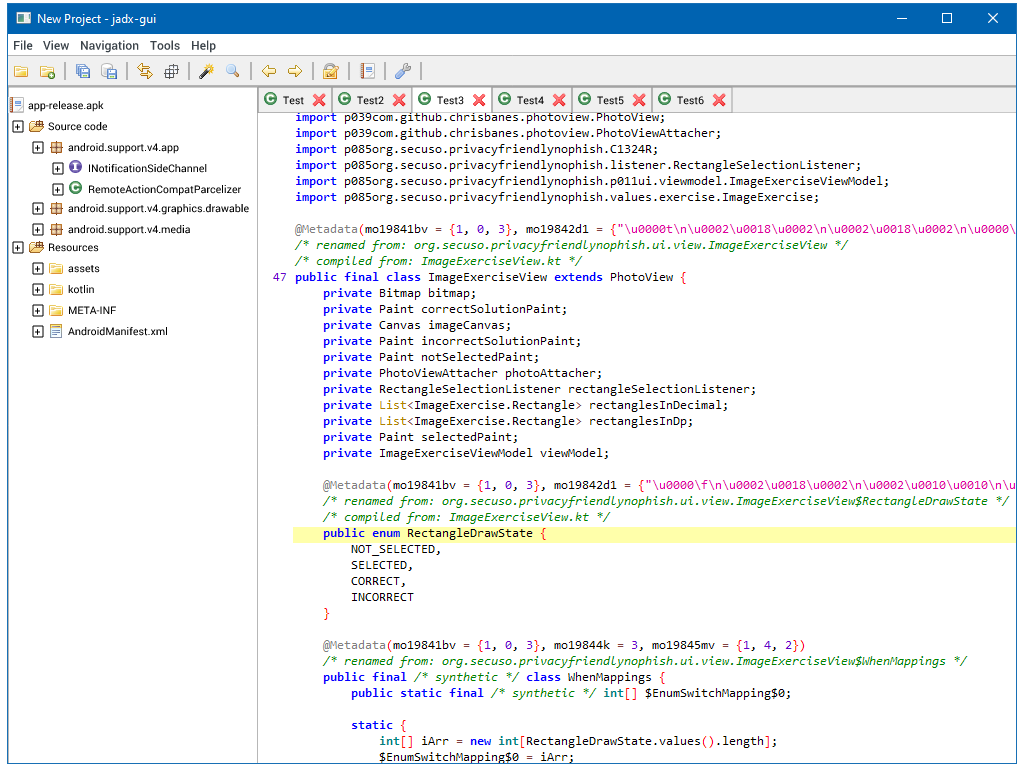
\includegraphics[height=.45\textheight]{bilder/jadx_mock_main.png}
    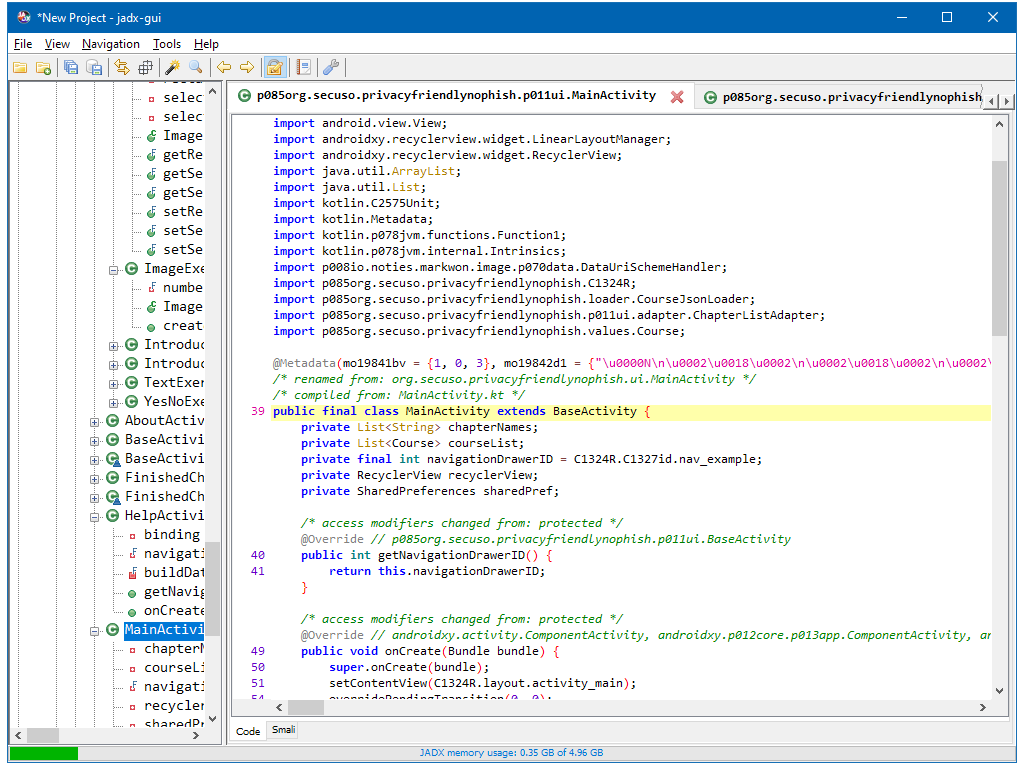
\includegraphics[height=.45\textheight]{bilder/jadx_main.png}
    \caption{Vergleich Hauptansicht: Mock (oben) und JADX (unten)}
    \label{fig:mock_comparison}
\end{figure}

\begin{figure}[p]
    \centering
    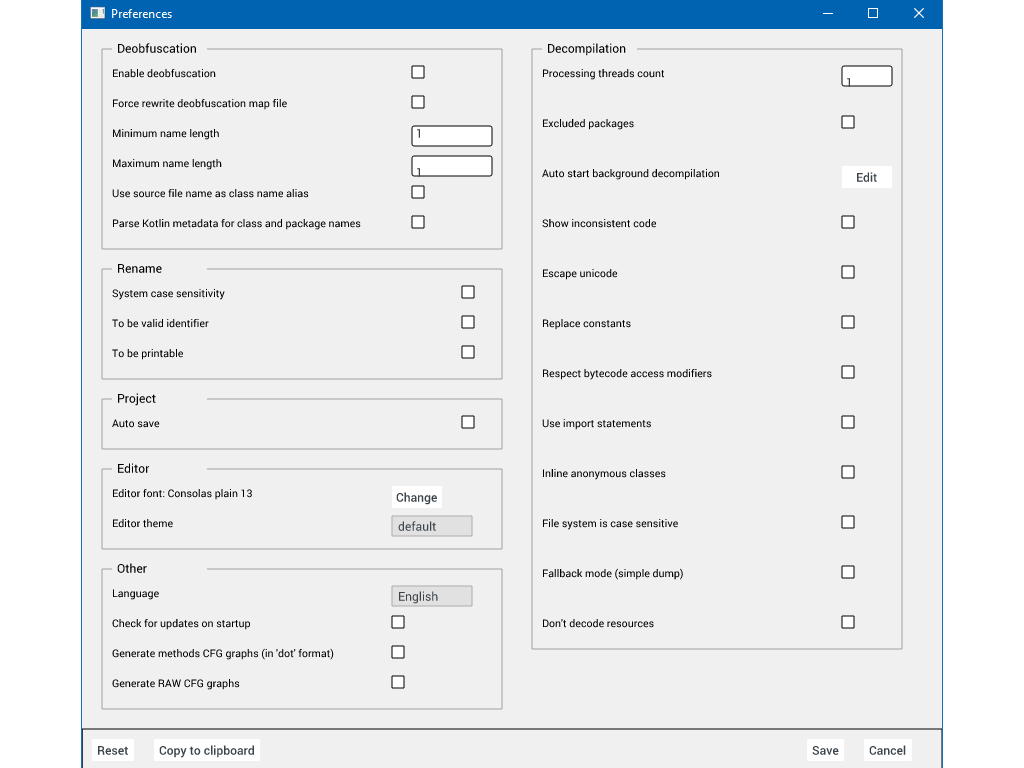
\includegraphics[height=.45\textheight]{bilder/jadx_mock_settings.png}
    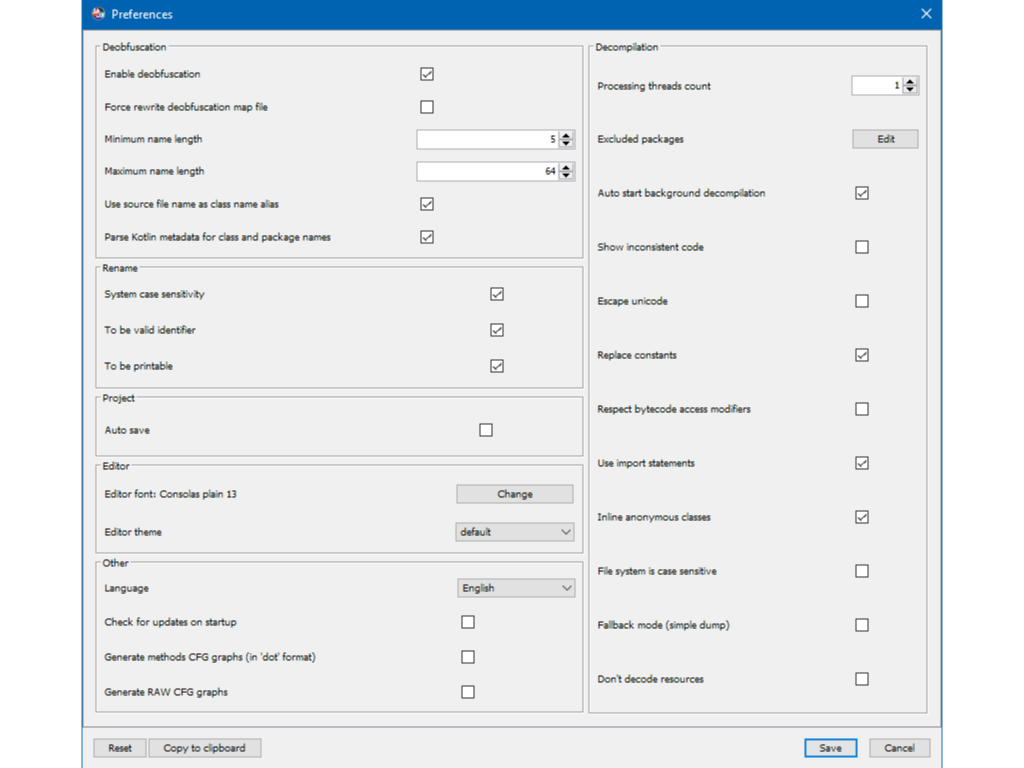
\includegraphics[height=.45\textheight]{bilder/jadx_settings.png}
    \caption{Vergleich Einstellungen: Mock (oben) und JADX (unten)}
    \label{fig:mock_settings_comparison}
\end{figure}

\begin{figure}[p]
    \centering
    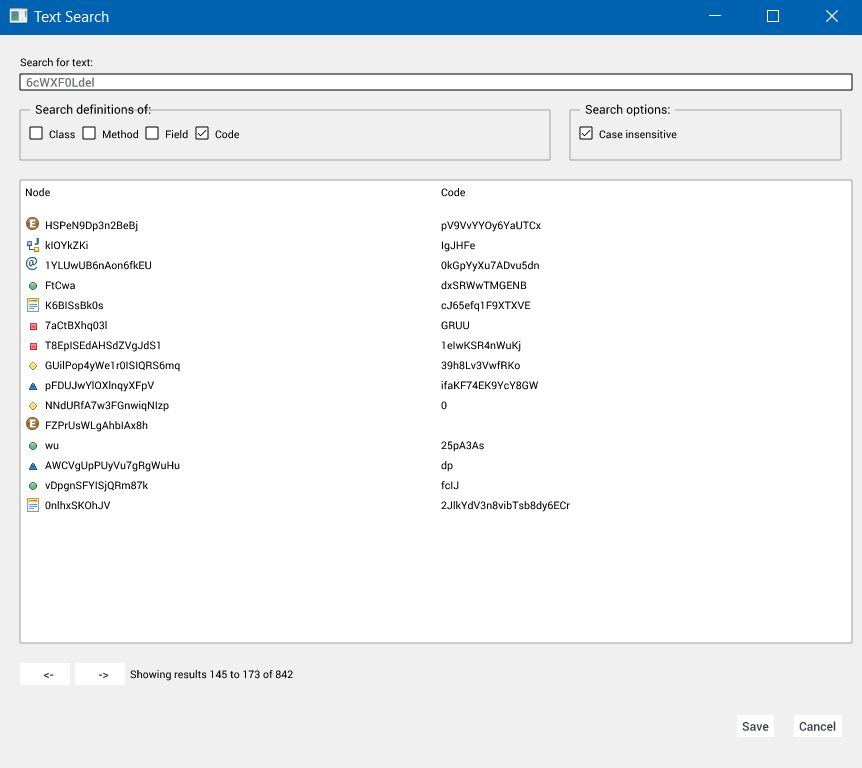
\includegraphics[height=.45\textheight]{bilder/jadx_mock_search.png}
    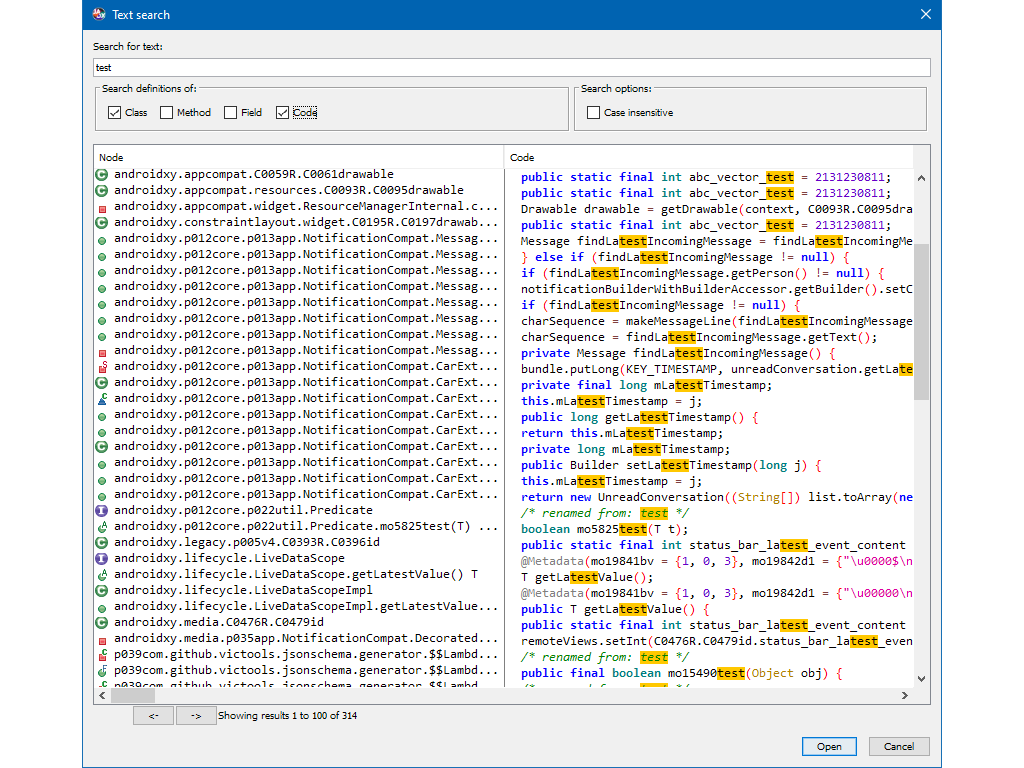
\includegraphics[height=.45\textheight]{bilder/jadx_search.png}
    \caption{Vergleich Text- / Klassensuche: Mock (oben) und JADX (unten)}
    \label{fig:mock_search_comparison}
\end{figure}





\subsection{Limitierungen}
\label{sec:mock_limitations}



Die Limitierungen der Umsetzung ergeben sich zunächst aus den Limitierungen und Fehlern von OrbTK, insbesondere der Rendering-Funktionen. Die meisten Elemente aus JADX sind nicht in OrbTK vorhanden, weshalb sie nachgebaut werden mussten. Das Design der JADX-Applikation, das sich an Windows-Designsprachen orientiert, konnte nicht immer exakt umgesetzt werden, sodass sich kleinere Abweichungen ergeben. OrbTK bietet die Möglichkeit Rahmen um Container innerhalb der Applikation zu ziehen, ähnlich wie sie in JADX oft verwendet werden. Selbst ein Rahmen der Breite \texttt{1}, die kleinste darstellbare Breite, erscheint dicker, als die innerhalb JADX verwendeten Rahmen. Weitere Features wie Schattierungseffekte oder gepunktete Linien (beispielsweise Verbindungslinien des Projekt-Baums in der Hauptansicht von JADX) sind nicht in OrbTK verfügbar.

\todo{Sind diese Abweichungein ein Problem? --> Später in der Arbeit genauer erörtern und Testset aus richtiger JADX-Applikation verwenden}

Die Funktionalität, um mehrere Fenster zu öffnen, ist in OrbTK grundsätzlich vorhanden. JADX verwendet dies beispielsweise um eine Volltext- oder Klassensuche durchzuführen. Das Öffnen zusätzlicher Fenstern ist in OrbTK jedoch aktuell noch sehr fehlerhaft. Wenn die Fenstergröße nach dem Öffnen beispielsweise durch den Mauszeiger verändert wird, wird der Inhalt des Fensters schwarz. Für diese Masterarbeit ist dieser Umstand jedoch kein Problem, da Fenster nur einmal gerendert werden, bevor sie als Bild gespeichert werden. Dadurch finden nach dem initialen Rendering keine Veränderungen mehr statt. Es existieren ähnliche Probleme bezüglich der Ausführung von Aktionen durch den Benutzer. In zusätzlichen Fenstern werden Mausklicks oft nicht registriert, sodass diese mehrfach durchgeführt werden müssen. Auch diese Fehler sind für diesen Anwendungsfall nicht relevant, da für die Experimente im Rahmen dieser Arbeit keine Aktionen mit der Maus durchgeführt werden. Alle Felder, die innerhalb von JADX erreichbar sind, werden vorausgefüllt.

\begin{figure}[h]
    \centering
    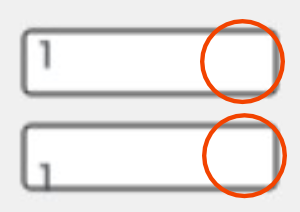
\includegraphics[scale=0.5]{bilder/NumericBoxPfeile.png}
    \caption{\texttt{NumericBox} mit fehlenden Buttons zum In- und Dekrementieren}
    \label{fig:numeric_box}
\end{figure}


In JADX werden darüber hinaus manche \gls{gui}-Elemente, wenn sie in einem zusätzlichen Fenster geöffnet werden, nicht angezeigt. Innerhalb der Box zur Eingabe numerischer Werte (\texttt{NumericBox}) werden die Buttons, durch welche der Wert in- oder dekrementiert werden kann, nicht angezeigt. Dies wird in Abb.~\ref{fig:numeric_box} dargestellt.
Weitere Unterschiede zwischen JADX und der Umsetzung des Mocks ergeben sich aus den Limitierungen von OrbTK in Verbindung mit der Umsetzungszeit. Wie in Abschnitt \ref{subsec:goal_mock} beschrieben ist, war es auch kein Ziel hinter der Entwicklung, JADX zu 100\% abzubilden. Viele Effekte, wie Schattierungen oder Verbindungslinien im Strukturbaum in der Hauptübersicht in Abb.~\ref{fig:mock_comparison}, sind so nicht in OrbTK vorhanden und nur mit unverhältnismäßigem Aufwand nachzubauen. Teilweise wurden auch \gls{gui}-Elemente implementiert, deren Design dem von JADX ähnlich ist, die jedoch keine Funktion haben. Ein Beispiel hierfür ist die Tab-Navigation über dem Editor. Die einzelnen Tabs sind nicht mit Daten hinterlegt, sodass bei einem Klick auf einen Tab nichts passiert. Da nur Abbilder der \gls{gui} verwendet werden und keine Aktionen ausgeführt werden, ist dies jedoch auch nicht notwendig. Features von JADX, wie die Speicherverbrauchsanzeige am unteren Fensterrand oder die kleinere Tabnavigation (\glqq Code\grqq\ und \glqq Smali\grqq ), wurden nicht umgesetzt.


% \begin{itemize}
%     \item Was wird für eine GUI benötigt?
%     \begin{itemize}
%         \item \textit{Welche Menüs?}
%         \item \textit{Welche Buttons? Wo platzieren?}
%         \item \textit{Styling?}
%     \end{itemize}
% \end{itemize}

\section{Implementierung der prozeduralen Generierung}
Die Ansichten der \gls{gui} müssen anschließend prozedural generiert werden. Da unstrukturierte, valide Ansichten zum Training der Autoencoder ausreichen, können zufällig neue Ansichten generiert werden. Wichtig hierbei ist, dass alle \gls{gui}-Elemente des Mocks, aber auch möglichst viele valide Konfigurationen und Kombinationen dieser Elemente, abgedeckt sind.
Im Proposal wurde die Frage aufgeworfen, ob die Generierung in Python oder Rust umgesetzt werden soll. Im ersten Fall müssten alle variablen Teile zur Verwendung durch Python freigegeben werden, womit die Schnittstelle zu Python komplexer werden würde. Dafür könnte der Quelltext, der die Generierung betrifft, in Python geschrieben werden, womit dieser Quelltext, wie im Proposal argumentiert, wartbarer, lesbarer und zugänglicher werden könnte. Letztere Argumentation hat sich im Lauf der Entwicklung als falsch herausgestellt. Durch die Kapselung in einen separatem Generator ist dieser sowohl wartbar als auch von der \gls{gui} separiert. Die Bedenken bezüglich der Lesbarkeit haben sich nicht bestätigt.
Daher wurde der Generator in Rust implementiert.

Um möglichst viel Variabilität von JADX abzudecken, ist ein hoher Grad an Randomisierung nötig. Jede Ansicht der Anwendung, die aus dynamischem Inhalt besteht, soll mit randomisiert generiertem Inhalt gefüllt werden. Dies betrifft den Projektbaum, die Tab-Navigation, den Inhalt des Editors, die Eingabefelder, Dropdown-Menüs~und~\mbox{Checkboxen}.

\subsection{Generator}
\label{subsec:generator}
Um \gls{gui}-Daten zu generieren, müssen sowohl der Inhalt als auch die Struktur erstellt werden. Die Struktur des Mocks bezeichnet dabei die geöffneten Fenster, die geöffneten Menüs und die Größe der Fenster. Die generierten Strukturelemente und deren Wahrscheinlichkeiten werden in Tab.~\ref{tab:window_probabilities} dargestellt. Die Wahrscheinlichkeit, dass ein zusätzliches Fenster angezeigt wird, beträgt $50\%$. Unter der Bedingung, dass \emph{kein} zusätzliches Fenster angezeigt wird, wird wiederum mit 50-prozentiger Wahrscheinlichkeit ein Menü angezeigt. Falls ein zusätzliches Fenster angezeigt wird, können gleichzeitig keine Menüs existieren. Die Gesamtwahrscheinlichkeit, ob ein solches Menü angezeigt wird, beträgt demnach $\frac{1}{4}$. Falls die Entscheidung, ob ein Menü bzw. Fenster  angezeigt wird, positiv ausfällt, wird die Entscheidung, welches Menü bzw. Fenster angezeigt wird, randomisiert anhand einer Gleichverteilung getroffen.

Der gesamte variable Inhalt des Mocks wird zufällig generiert. Dies bedeutet, dass alle Eingabefelder, Dropdown-Menüs und Checkboxen zufällig befüllt werden. Die möglichen Werte für die einzelnen Variationspunkte werden in Tab.~\ref{tab:variation_fields} beschrieben. In Tab.~\ref{tab:variation_components} werden weitere Komponenten beschrieben, deren Struktur generiert wird, die jedoch auch aus mehreren randomisiert generierten Bausteinen bestehen.

Die Wahrscheinlichkeiten wurden so gewählt, dass Ansichten mit einer höheren Komplexität häufiger gezeigt werden, als Ansichten mit einer geringeren Komplexität. Ein Menü mit einigen statischen Icons und statischem Text ist dabei wesentlich weniger komplex, als ein größeres Fenster mit entsprechend mehr und vor allem dynamisch generiertem Inhalt. Fenster wurden deshalb gegenüber Menüs im Generator stärker gewichtet ($p_{fenster}=\frac{1}{12}$ gegenüber $p_{menu}=\frac{1}{20}$). Die Menüs sowie die Fenster untereinander werden gleich häufig angezeigt, um ein gleichmäßiges Lernen der Elemente zu gewährleisten.

\subsection{Anmerkung}
An dieser Stelle ist es wichtig zu erwähnen, dass sich die Wahrscheinlichkeitsverteilung \emph{nicht} an der Wahrscheinlichkeitsverteilung bei einer realistischen Nutzung orientiert. Das Ziel des Generators ist es, das Training zu optimieren, und nicht, eine realitätsnahe Wahrscheinlichkeitsverteilung abzubilden. Ein häufiges Problem bei maschinellem Lernen ist, dass Randfälle in den Trainingsdaten unterrepräsentiert sind, wie etwa im Bereich des autonomen Fahrens~\cite{karunakaranEfficientStatisticalValidation2020}. Ein Vorteil des Ansatzes dieser Masterarbeit ist es, Randfälle beliebig und einfach stärker gewichten zu können. Falls notwendig kann diese Gewichtung auch nachträglich durch Neuerstellung des Datensatzes verändert werden.

% \newpage

\begin{figure}[p]
    \centering
    \renewcommand*{\arraystretch}{1.5}
    \begin{minipage}{\textwidth}
    \captionof{table}{Strukturelemente mit dazugehöriger Anzeigewahrscheinlichkeit}
    \label{tab:window_probabilities}
    \smallskip
    \begin{tabularx}{\textwidth}{ lX }
        \toprule
        Strukturelement & Anzeigewahrscheinlichkeit \\
        \hline
        kein zusätzliches Fenster & $P(X=kein Fenster) = 0,5$ \\
        Einstellungsfenster & $P(X=Einstellungen) = \frac{1}{12}$\\
        Textsuchfenster & $P(X=Textsuche) = \frac{1}{12}$ \\
        Klassensuchfenster & $P(X=Klassensuche) = \frac{1}{12}$ \\
        Suchfenster für Suche nach Benutzung & $P(X=Benutzungssuche) = \frac{1}{12}$ \\
        Fenster zur Umbenennung & $P(X=Umbenennung) = \frac{1}{12}$\\
        \glqq Über\grqq -Fenster & $P(X=\ddot{U}ber) = \frac{1}{12}$\\
        Kein Menü & $P(Y=keinMen\ddot{u})=0,25$, $P(keinFenster | Y=keinMen\ddot{u}) = 0,5$\footnote{$P(\neg keinFenster | Y=keinMen\ddot{u}) = 1 $} \\
        File-Menü & $P(Y=FileMen\ddot{u})=0,05$, $P(keinFenster | Y=FileMen\ddot{u}) = 0,1$\footnote{ $P(\neg keinFenster | Y=FileMen\ddot{u}) = P(\neg keinFenster | Y=ViewMen\ddot{u}) = \\ P(\neg keinFenster | Y=NavigationMen\ddot{u}) = P(\neg keinFenster | Y=ToolsMen\ddot{u}) = \\ P(\neg keinFenster | Y=HelpMen\ddot{u}) = 0 $\label{fn:tab:negate_prop}} \\
        View-Menü & $P(Y=ViewMen\ddot{u})=0,05$, $P(keinFenster | Y=ViewMen\ddot{u}) = 0,1$\footref{fn:tab:negate_prop} \\
        Navigation-Menü & $P(Y=NavigationMen\ddot{u})=0,05$, $P(keinFenster | Y=NavigationMen\ddot{u}) = 0.1$\footref{fn:tab:negate_prop} \\
        Tools-Menü & $P(Y=ToolsMen\ddot{u})=0,05$, $P(keinFenster | Y=ToolsMen\ddot{u}) = 0,1$\footref{fn:tab:negate_prop}\\
        Help-Menü & $P(Y=HelpMen\ddot{u})=0,05$, $P(keinFenster | Y=HelpMen\ddot{u}) = 0,1$\footref{fn:tab:negate_prop}\\
        \bottomrule
    \end{tabularx}
\end{minipage}
\end{figure}

%     \footnotetext[20]{ $P(\neg keinFenster | Y=FileMen\ddot{u}) = P(\neg keinFenster | Y=ViewMen\ddot{u}) = \\ P(\neg keinFenster | Y=NavigationMen\ddot{u}) = P(\neg keinFenster | Y=ToolsMen\ddot{u}) = \\ P(\neg keinFenster | Y=HelpMen\ddot{u}) = 0 $\label{fn:tab:negate_dprop}}


% \end{figure}

\begin{table}[p]
    \centering
    \caption{\glsxtrshort{gui}-Elemente mit generiertem Inhalt}
    \label{tab:variation_fields}
    \smallskip

\begin{tabularx}{\textwidth}{ XXX }
    \toprule
    Variationspunkt & Art der Befüllung & Inhaltsart \\
    \hline
    Checkbox & Zufällige Markierung & Ja/Nein \\
    Dropdown-Menü & Zufällige Auswahl & Statische Elemente \\
    Numerisches Feld & Zufällige Zahl & Realistischer Zahlenbereich (Bsp: 1..100) \\
    Text(-feld) & Zufälliger Text & Alphanumerischer Text mit Länge in bestimmtem Bereich \\
    Icon & Zufälliges Icon & Icons aus JADX (je nach Kontext nur Icons für Dateien oder Entitäten) \\
    \bottomrule
\end{tabularx}


\end{table}

\begin{table}[p]
    \centering
    \caption{JADX-Komponenten mit generierter Struktur und Inhalt}
    \label{tab:variation_components}
    \smallskip

\begin{tabularx}{\textwidth}{ XXX }
    \toprule
    Variationspunkt & Elemente & Art der Befüllung  \\
    \hline
    Tab-Navigation & Tabs bestehend aus Icon und Text & 1..10 Tabs \\
    Projektbaum & Einträge aus Icon und Text sowie Kindelementen & Baumstruktur: Jedes Element hat bis zu 10 Kindelemente, max. 100 Elemente \\
    Suchergebnisse & Einträge aus Icon sowie 2 Texten (In JADX Name der Entität und ein Code-Ausschnitt ) & Max. 20 Einträge (zeilenweise) \\

    \bottomrule
\end{tabularx}
\end{table}

% \begin{itemize}
%     \item Was ist das?
%     \begin{itemize}
%         \item Generierung der GUI über Parameter und Zufall
%         \item Implementierung in Python oder Rust?
%     \end{itemize}
%     \item Warum prozedural Generieren?
%     \item Was ist dabei wichtig?
% \end{itemize}
\section{Implementierung von Python-Bindings}
Im Proposal zu dieser Masterarbeit wurde vorgeschlagen Bindings zu schreiben, um eine Verwendung des Generators in Python zu ermöglichen.
Python-Bindings definieren die Schnittstelle, um Bibliotheken anderer Programmiersprachen in Python aufzurufen. Diese Technik wird häufig genutzt um die Geschwindigkeitsvorteile von in C, C++ oder Rust entwickelten Bibliotheken auch in Python zu nutzen.

Ursprünglich war es vorgesehen, Python-Bindings zu entwickeln, um den Generator innerhalb des PyTorch-Quelltexts zu starten. Im Zug des Entwicklungsprozesses traten jedoch Probleme mit Speicherlecks durch OrbTK bei der wiederholten Generierung von Bildern auf. Daher traf ich die Entscheidung, auf die Entwicklung von Python-Bindings zu verzichten und den Generator so umzubauen, dass er nur ein einziges Bild generiert. Ein Bash-Skript startet den Generator dann so oft, bis der Datensatz fertiggestellt ist. Der Generator wird so jedes Mal in einem neuen Prozess gestartet, wodurch keine Speicherlecks und Probleme mit der \gls{cpu}-Auslastung auftreten können. In der Praxis führt dies nicht zu Einschränkungen, da der Datensatz in der Regel nur ein Mal erstellt wird und später nur noch verwendet wird. Es kommt somit nicht zu einem nennenswertem Mehraufwand bei der Entwicklung der Autoencoder.

% Aktuell ist der Generator so aufgebaut, dass für jedes Bild eine neue Instanz von OrbTK in einem eigenen Thread gestartet wird, von welcher ein Screenshot erstellt wird. Für einen Datensatz von 1000 Bildern werden daher 1000 Instanzen geöffnet und geschlossen. Das Schließen der Instanzen scheint jedoch zum aktuellen Zeitpunkt nicht fehlerfrei zu funktionieren und resultiert in einem Speicherleck. Die \gls{cpu}-Auslastung steigt ebenso immer weiter an, bis sie 100\% erreicht und die Generierung der Bilder immer langsamer funktioniert. Die einzige Lösung für dieses Problem ist es, jeweils einen eigenen Prozess pro OrbTK-Instanz zu starten.


% \begin{itemize}
%     \item Warum?
%     \item Was ist das?
%     \begin{itemize}
%         \item Rust Code der von Python (beispielsweise über Pip Package) aufgerufen werden kann
%         \item Deklarierte Schnittstelle
%     \end{itemize}
%     \item Wie funktioniert das?
%     \begin{itemize}
%         \item PyO3 (\url{https://pyo3.rs})
%         \item Siehe Beispiele
%     \end{itemize}
% \end{itemize}

\section{Fazit}
Das Ergebnis der Entwicklung des Mocks ist insgesamt zufriedenstellend. Die Abweichungen zwischen JADX und dem Mock sind bis auf wenige Features und den Betriebssystemfunktionalitäten gering. Inwiefern diese Abweichungen für die Ergebnisse eine Role spielen wird in Kapitel~\ref{cha:autoencoder} besprochen.
Die Bewertung, ob solche Mocks in Zukunft eingesetzt werden sollen, fällt jedoch negativ aus. OrbTK bereitet insgesamt durch ein schlechtes Layout-System, Speicherlecks, aktuell keiner Offscreen-Rendering-Unterstützung und andere Bugs zu viele Probleme. Es ist nur mit Aufwand möglich, einen solchen Mock zu erstellen, der dann auch produktiv eingesetzt werden kann. Alle weiteren untersuchten Frameworks sind ebenfalls noch in einem frühen Stadium und benötigen oft eine \gls{gpu}. Inwiefern letztere durch einen Software-Renderer ersetzt werden kann, ist zum jetzigen Stand zwar unklar, wäre jedoch auch nicht mehr als ein Workaround und damit prinzipiell nicht optimal.
\chapter{Entwicklung der Autoencoder}
\label{cha:autoencoder}
Die am \gls{fzi} entwickelten \glspl{ctrnn} können nur schlecht mit sehr hochdimensionalen Daten wie Ansichten von \glspl{gui} umgehen. \todo{Beleg - besser nach oben schieben? (evtl in Ziel oder in Absatz am Anfang des Kapitels)} Daher sollen Autoencoder eingesetzt werden, um die Dimensionalität der Eingabedaten zu verringern. Das Ziel ist es, eine möglichst effiziente Kodierung einer \gls{gui} zu erreichen, um die \glspl{ctrnn} sowohl effektiver als auch schneller zu trainieren.
Zu diesem Zweck wurden mehrere Autoencoder-Architekturen implementiert und evaluiert, inwiefern sie sich für diesen Einsatzzweck eignen.

Die Architekturen unterscheiden sich in der Anzahl, Abfolge und in der Art der einzelnen Schichten (beispielsweise Fully-Connected- oder Convolutional-Schichten). Des Weiteren wurden unterschiedliche Aktivierungsfunktionen eingesetzt. Die Autoencoder setzen Teile der Anforderungen an einen \gls{vae} um, können jedoch nicht als \gls{vae} bezeichnet werden. Die in Abschnitt~\ref{subsubsec:vae-layer} eingeführte \gls{vae}-Schicht ist jeweils vorhanden, während dort ebenfalls beschriebene Kullback-Leibler-Divergenz nicht verwendet wurde. Um dies umzusetzen, müssen die Kullback-Leibler-Divergenz zur Fehlerfunktion hinzugefügt und die Autoencoder neu trainiert werden.

Die Architekturen werden zunächst einzeln vorgestellt und verglichen. Anschließend werden die Auswahl des Datensatzes und der Parameter der Experimente beschrieben und die einzelnen Experimente vorgestellt. Zum Schluss folgt die Erörterung der Ergebnisse.



% \todo{welche?}
% \begin{itemize}
%     \item Warum?
%     \begin{itemize}
%         \item Möglichst effiziente Kodierung einer GUI
%         \item Performance --> extrem aufwändig auf hochdimensionalen Pixeldaten zu lernen!
%     \end{itemize}
%     \item Mehrere Architekturen
% \end{itemize}

\section{Autoencoder-Architekturen}
Alle Architekturen wurden mit der Bibliothek PyTorch\footnote{\url{https://pytorch.org}, letzter Zugriff: 13.12.2021} in Version 1.9.1 implementiert. Dabei wurden die vorimplementierten Schichten aus \texttt{torch.nn} und die Aktivierungsfunktionen aus den Modulen \texttt{torch.nn.functional} bzw. \texttt{torch} entnommen. Die einzelnen Architekturen werden in den Abb.~\ref{fig:arch1} bis \ref{fig:arch4} dargestellt, wobei die \gls{vae}-Schicht aus Gründen der Übersichtlichkeit nicht abgebildet wird. Deren Funktionsweise kann in Abschnitt~\ref{subsubsec:vae-layer} nachgelesen werden.

\begin{figure}
    \centering
    \begin{minipage}{0.45\textwidth}
        \centering
        % \def\svgwidth{\linewidth}
        \scalebox{0.75}{\input{arch1.pdf_tex}}
        \caption{Illustration der Architektur des Autoencoders 1 ohne VAE-Schicht}
        \label{fig:arch1}
    \end{minipage}\hfill
    \begin{minipage}{0.45\textwidth}
        \centering
        % \def\svgwidth{\linewidth}
        \scalebox{0.75}{\input{arch2.pdf_tex}}
        \caption{Illustration der Architektur des Autoencoders 2 ohne VAE-Schicht}
        \label{fig:arch2}
    \end{minipage}
\end{figure}

\begin{figure}
    \centering
    \begin{minipage}{0.45\textwidth}
        \centering
        % \def\svgwidth{\linewidth}
        \scalebox{0.75}{\input{arch3.pdf_tex}}
        \caption{Illustration der Architektur des Autoencoders 3 ohne VAE-Schicht}
        \label{fig:arch3}
    \end{minipage}\hfill
    \begin{minipage}{0.45\textwidth}
        \centering
        % \def\svgwidth{\linewidth}
        \scalebox{0.75}{\input{arch4.pdf_tex}}
        \caption{Illustration der Architektur des Autoencoders 4 ohne VAE-Schicht}
        \label{fig:arch4}
    \end{minipage}
\end{figure}

\label{Autoencoder2VAEMediumConvBigKernel}
% AE 3b7d5453ce41baeba6fcab6937df2c16a4fc9523
\textbf{Autoencoder~\customlabel{a1}{1}} wird in Abb.~\ref{fig:arch1} dargestellt. Er realisiert die von Kies~\cite{kiesEntwicklungUndAnalyse2020} entwickelte Autoencoder-Architektur~4, welche Kies als die Beste der in der Bachelorarbeit entwickelten Architekturen bezeichnete. Der Encoder-Teil dieses Autoencoders besteht aus drei Convolutional-Schichten sowie zwei Fully-Connected-Schichten. Am Übergang zwischen den beiden Schichttypen findet ein Flattening, wie in Abschnitt~\ref{subsec:flattening} beschrieben, statt. Der Decoder ist entsprechend symmetrisch aufgebaut. Diese Architektur wurde gegenüber der von Kies insofern angepasst, dass den größeren Eingabebildern in dieser Masterarbeit Rechnung getragen werden kann. Daher enthält der Autoencoder eine weitere Convolutional-Schicht und die einzelnen Schichten wurden deutlich vergrößert.\linebreak Die Filtergröße der ersten Schicht wurde von 5x5 auf 32x32 vervielfacht und die Max-Pooling-Schichten von 4x4 auf 8x8 vergrößert. Die äußerste Fully-Connected-Schicht ist nun 10.000 statt 5.200 Neuronen breit. Die Vergrößerung des Kernels in der äußersten Schicht wurde durchgeführt, um eine Anpassung hinsichtlich der kleinsten Bildelemente zu erreichen. Diese sind hier deutlich komplexer als die kleinsten Elemente in der Arbeit von Kies. Das Bottleneck ist aufgrund der höheren Komplexität der Daten durch die größeren Bilder mit 60 Neuronen doppelt so groß wie bei Kies. Die Aktivierungsfunktionen der einzelnen Schichten sind identisch und entsprechen der ReLU-Funktion im Fall der Convolutional-Schichten im Encoder und der Sigmoid-Funktion im Fall der Fully-Connected-Schichten.

\label{Autoencoder2VAEBigConvNoFully}
% AE 3547a5236c708c442558e4691d60e000893a122f
\textbf{Autoencoder~\customlabel{a2}{2}} wird in Abb.~\ref{fig:arch2} dargestellt. Im Vergleich zu Autoencoder~\ref{a1} enthält dieser Autoencoder, bis auf die \gls{vae}-Schicht, keine Fully-Connected-Schichten. Stattdessen sind die Convolutional-Schichten entsprechend größer gewählt und wurden um eine zusätzliche Schicht ergänzt. Insgesamt besteht der Autoencoder im Encoder-Teil somit aus vier Convolutional-Schichten bzw. im Decoder aus vier Transposed-Convolution-Schichten. Das Bottleneck besteht aus 320 Neuronen und ist somit deutlich größer. Ein weiterer signifikanter Unterschied ist der mit einer Größe von 12x12 deutlich kleinere Filter in der ersten Convolutional-Schicht. Die Filtergrößen wurden ausgewogener gestaltet um eine gleichmäßige Verkleinerung der Neuronenanzahl von Schicht zu Schicht zu erreichen. Die Aktivierungsfunktionen der einzelnen Schichten wurden verändert und entsprechen nun der LeakyReLU-Funktion im Fall der Convolutional-Schichten mit Ausnahme der letzten Schicht. In dieser wurde die Sigmoid-Funktionen verwendet.

\label{Autoencoder2VAEMediumConvSmallKernelBigBottleneck}
% AE 13694de2d2424a379efaa48beb645d2dabcb4604
\textbf{Autoencoder~\customlabel{a3}{3}} ist an Autoencoder~\ref{a1} angelehnt und wird in Abb.~\ref{fig:arch3} dargestellt. Im Vergleich zu Autoencoder~\ref{a1} zeichnet sich dieser durch einen deutlich größeren Anteil an Fully-Connected-Schichten aus. Deren Anzahl ist zwar identisch, die einzelnen Schichten sind jedoch deutlich größer. Die erste Convolutional-Schicht hat mit einer Größe von 16x16 einen entsprechend kleineren Filter und die ersten beiden Max-Pooling-Schichten wurden in ihrer Größe von 8x8 auf 6x6 und 4x4 reduziert. Damit stellt dieser Autoencoder eine Art Gegenentwurf zu Autoencoder~\ref{a2} dar. Hierbei wird die tanh-Funktion als Aktivierungsfunktion der Fully-Connected-Schichten eingesetzt. Die LeakyReLU-Funktion kommt im Fall der Convolutional-Schichten bis auf die letzte Schicht zum Einsatz, in der die Sigmoid-Funktion verwendet wurde.

\label{AutoencoderVAEMediumConvSmallKernel}
% AE 012f2d5ce7ab9b1e437ffe10fc120ec1107fb3a6
\textbf{Autoencoder~\customlabel{a4}{4}} ist eine Abwandlung von Autoencoder~\ref{a3} und wird in Abb.~\ref{fig:arch4} dargestellt. Auch dieser Autoencoder besteht aus drei Convolutional- und zwei Fully-Connected-Schichten, von denen die Convolutional-Schichten im Encoder identisch sind zu Autoencoder~\ref{a3}. Im Unterschied zu jenem Autoencoder wird hier die Sigmoid-Funktion für alle Transposed-Convolutional-Schichten des Decoders verwendet. Des Weiteren wurde die Breite des Bottlenecks von 360 Neuronen auf 180 Neuronen halbiert.

\section{Datensatz}
Der Datensatz wurde mit dem Generator aus Kapitel~\ref{cha:gui} erstellt und besteht aus insgesamt 191.124 Bildern. Die Abmessungen der einzelnen Bilder betragen 935x900 Pixel.
Zur Durchführung der Experimente wurde der Datensatz in einen Trainingsdatensatz bestehend aus 133.786 Bildern (70\%) und einen Testdatensatz bestehend aus 57.338 Bildern (30\%) aufgeteilt. Die Aufteilung erfolgte durch die Zuteilung zufälliger Bilder zum Testdatensatz. Die restlichen Bilder bildeten den Trainingsdatensatz. Wie in Abschnitt~\ref{subsec:generator} beschrieben, ist es wichtig zu betonen, dass die Zusammensetzung des Datensatzes sich nicht an realem Nutzungsverhalten sondern an der Komplexität der \gls{gui}-Elemente orientiert um das Lernen zu optimieren.

\section{Hyperparameter und Lernverfahren}
\label{sec:hyperparameter}
Alle Autoencoder wurden mit dem Trainingsdatensatz trainiert. Dabei kam das Adamax-Verfahren zum Einsatz, welches in Abschnitt~\ref{subsec:lernverfahren} beschrieben wird. Als initiale Lernrate wurde der von PyTorch standardmäßig eingestellte Wert $0,002$ verwendet. Im Rahmen des Trainings wurde die in PyTorch vorhandene Implementierung der binären Kreuzentropie (\gls{bce}) (\texttt{torch.nn.BCELoss})  als Fehlerfunktion verwendet.

Alle Autoencoder wurden mit dem gesamten Trainingsdatensatz trainiert, wobei Autoencoder~\ref{a1} in 2 Epochen und die restlichen Autoencoder in 3 Epochen trainiert wurden. Insgesamt verarbeitete jeder Autoencoder damit 267.572 bzw. 401.358 Bilder während des Trainings. Die Batch-Größe betrug in der Regel 16 Bilder. Lediglich für Autoencoder~\ref{a3} musste die Größe der Batches aus Speichergründen auf 12 Bilder pro Batch verringert werden, da der Speicher der verwendeten \gls{gpu} sonst nicht ausgereicht hätte.

\section{Trainingsverlauf}
Die Werte der Fehlerfunktion wurden im Verlauf des Trainings gespeichert und werden in Abb.~\ref{fig:training_loss} dargestellt. Diese wurden dabei über den Verlauf von 25 Batches aufgezeichnet und gemittelt. Jeder einzelne gespeicherte Wert entspricht damit dem Mittelwert des Fehlers bei $25 \cdot b$ Bildern, wobei $b$ die Batch-Größe bezeichnet. Es ist zu beachten, dass die Werte im Mittel dennoch vergleichbar bleiben, lediglich die einzelnen Abweichungen können bei Autoencoder~\ref{a3} aufgrund der geringeren Batchgröße größer ausfallen. Da Autoencoder~\ref{a1} nur in 2 Epochen trainiert wurde, umfassen die Werte dieses Autoencoders nur $\frac{2}{3}$ der x-Achse des Diagramms. Wie ersichtlich wird, stagnieren die Werte dieses Autoencoders, sodass eine weitere Epoche nicht zu einer nennenswerten Verringerung des Fehlers beigetragen hätte.
In Abb.~\ref{fig:training_loss_2500} wird darüber hinaus der Verlauf der Ergebnisse der Fehlerfunktion für die letzten 2500 Bilder für jeden Autoencoder dargestellt. Es ist erkennbar, dass Autoencoder~\ref{a3} und \ref{a4} in etwa gleich niedrige Werte aufweisen, während die Werte von Autoencoder~\ref{a1} und \ref{a2} darüber liegen. Daneben verhalten sich die Kurven der Autoencoder~\ref{a1}, \ref{a2} und \ref{a4} synchron, während die von Autoencoder~\ref{a3} davon abweicht. Dies ist kein Zeichen für ein gegenüber den anderen Autoencodern unterschiedliches Verhalten. Stattdessen kann man diesen Effekt durch die unterschiedliche Batch-Größe erklären, die eine andere Aufteilung der Einträge im Diagramm bedingt.

\begin{figure}[htbp]
    \centering
    \begin{center}

        \rotatebox{90}{%
          \begin{minipage}{.85\textheight}
            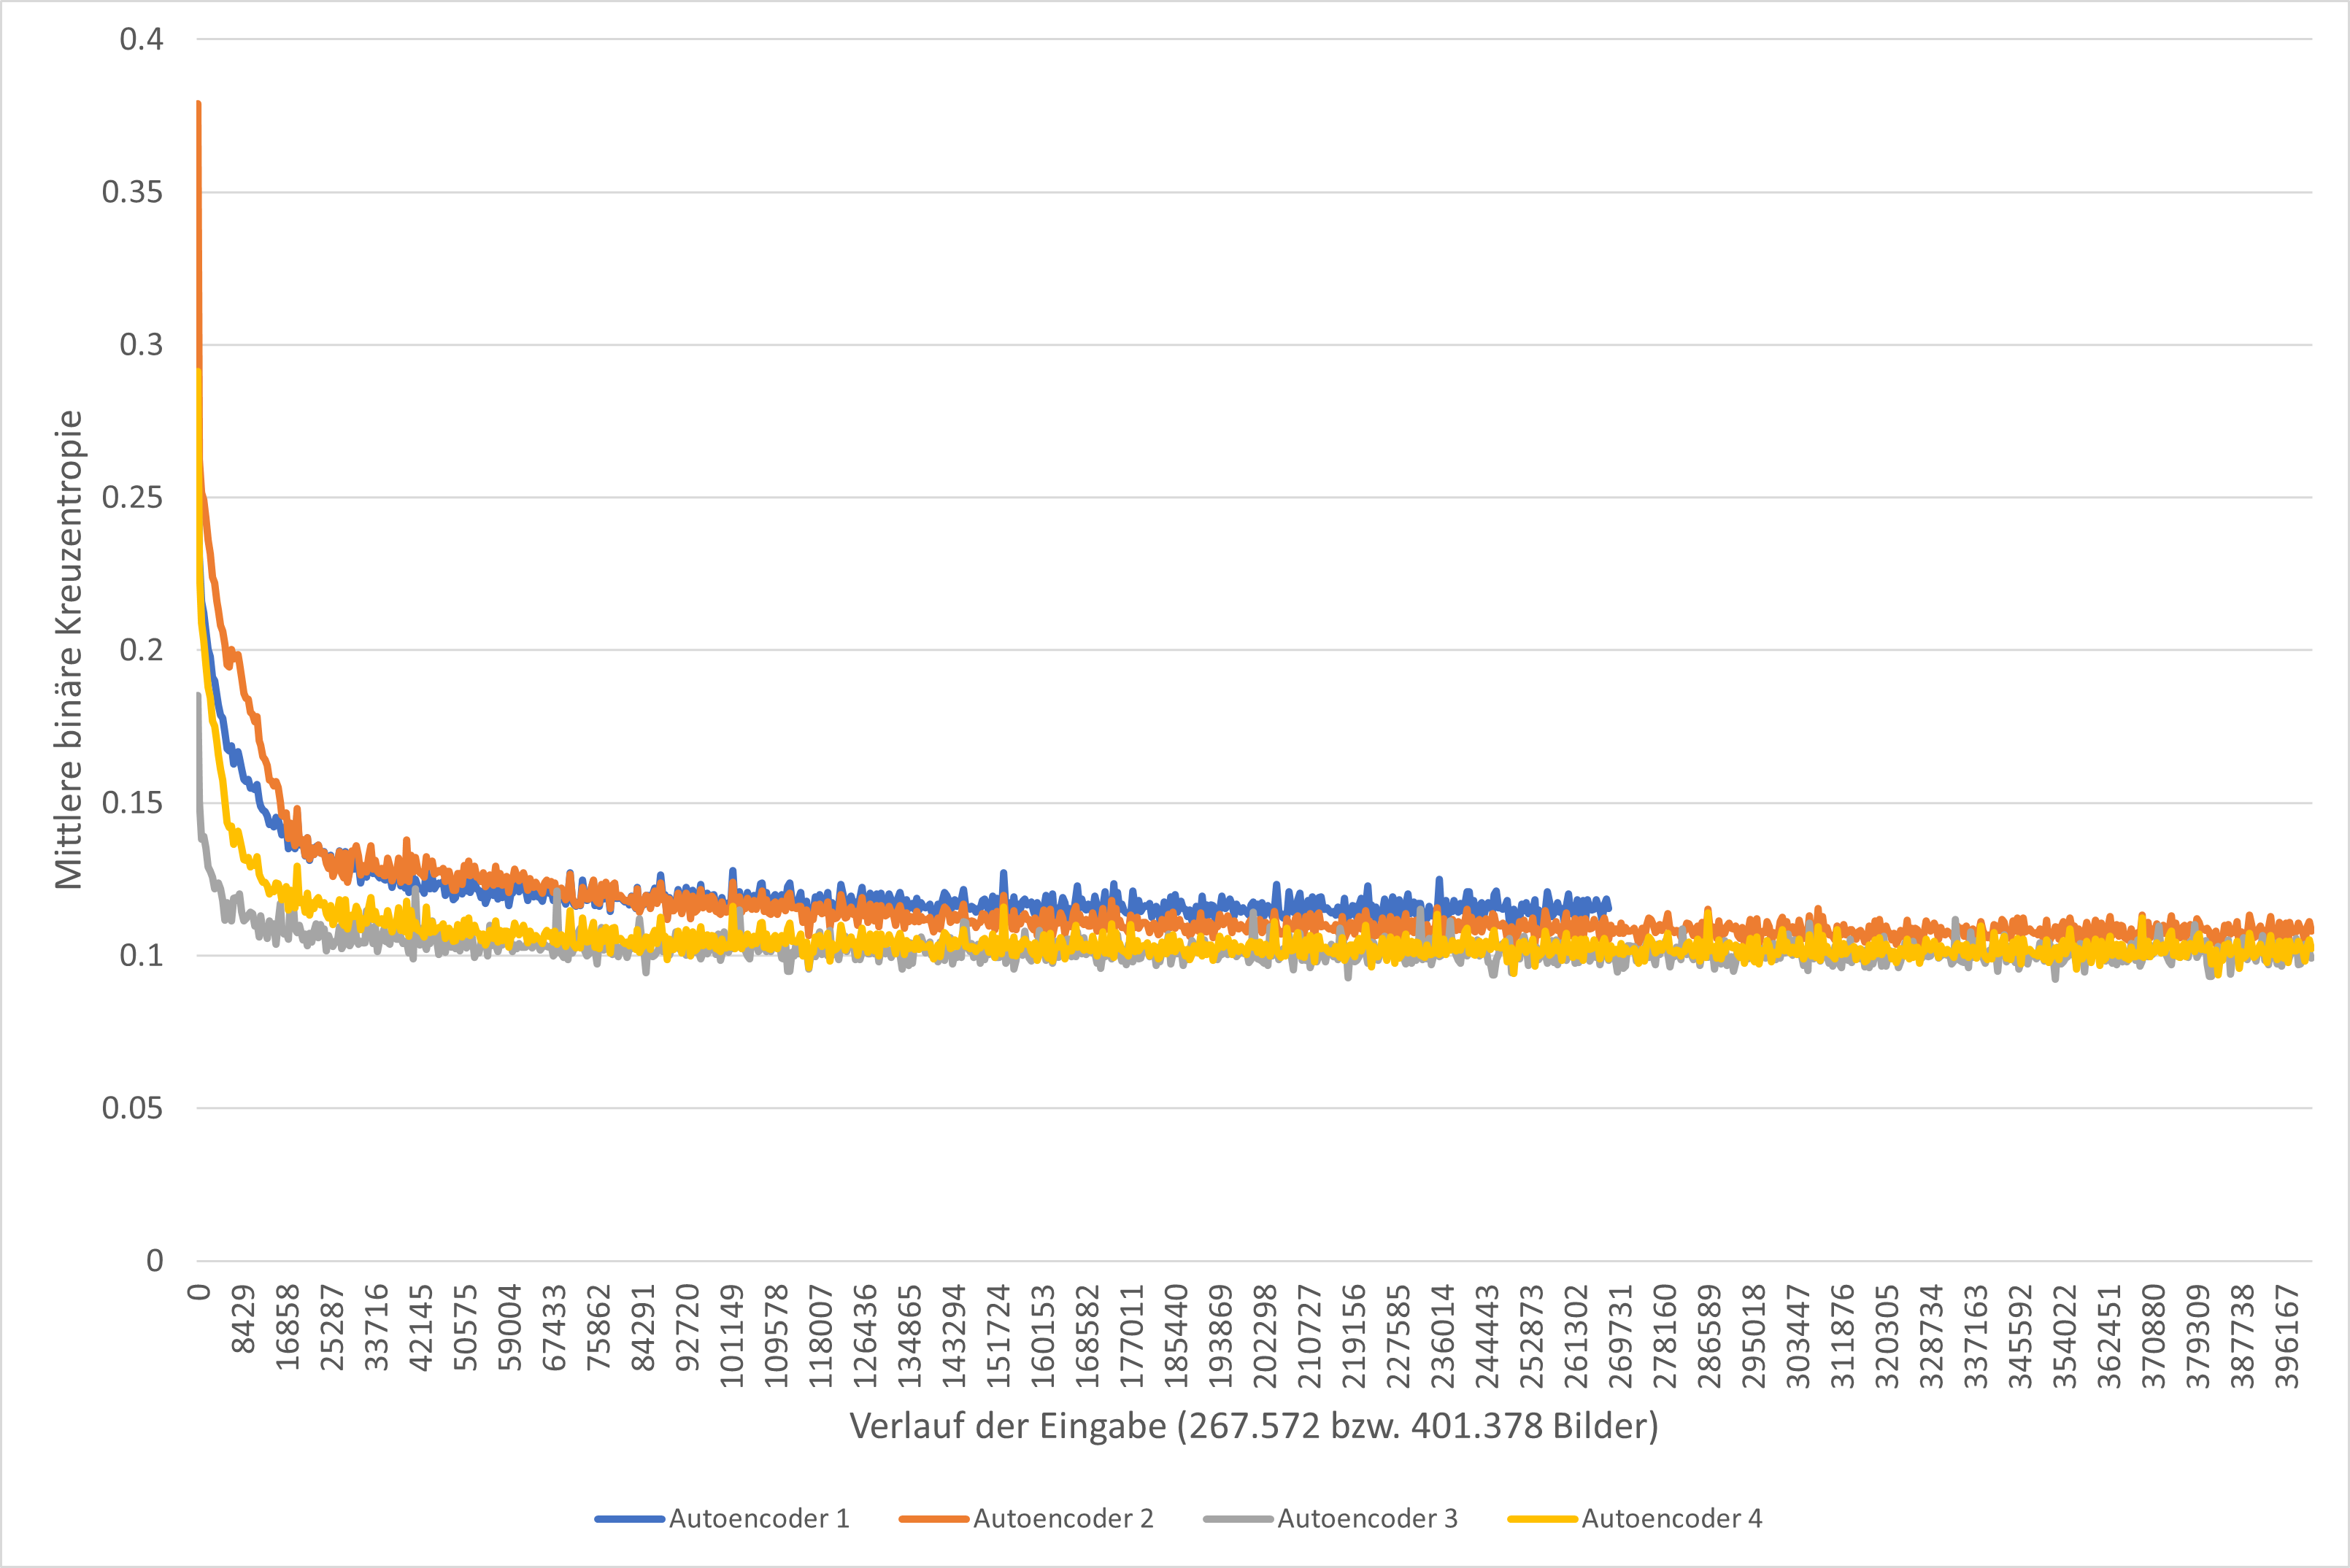
\includegraphics[width=\textwidth]{bilder/training_diagram.png}
            \captionof{figure}{Über 300 bzw. 400 Eingaben gemittelte binäre Kreuzentropie im Lauf des Trainings}
            \label{fig:training_loss}
                \renewcommand{\arraystretch}{1.5}
        \end{minipage}
        }
        \end{center}
\end{figure}


\begin{figure}[htbp]
    \centering
    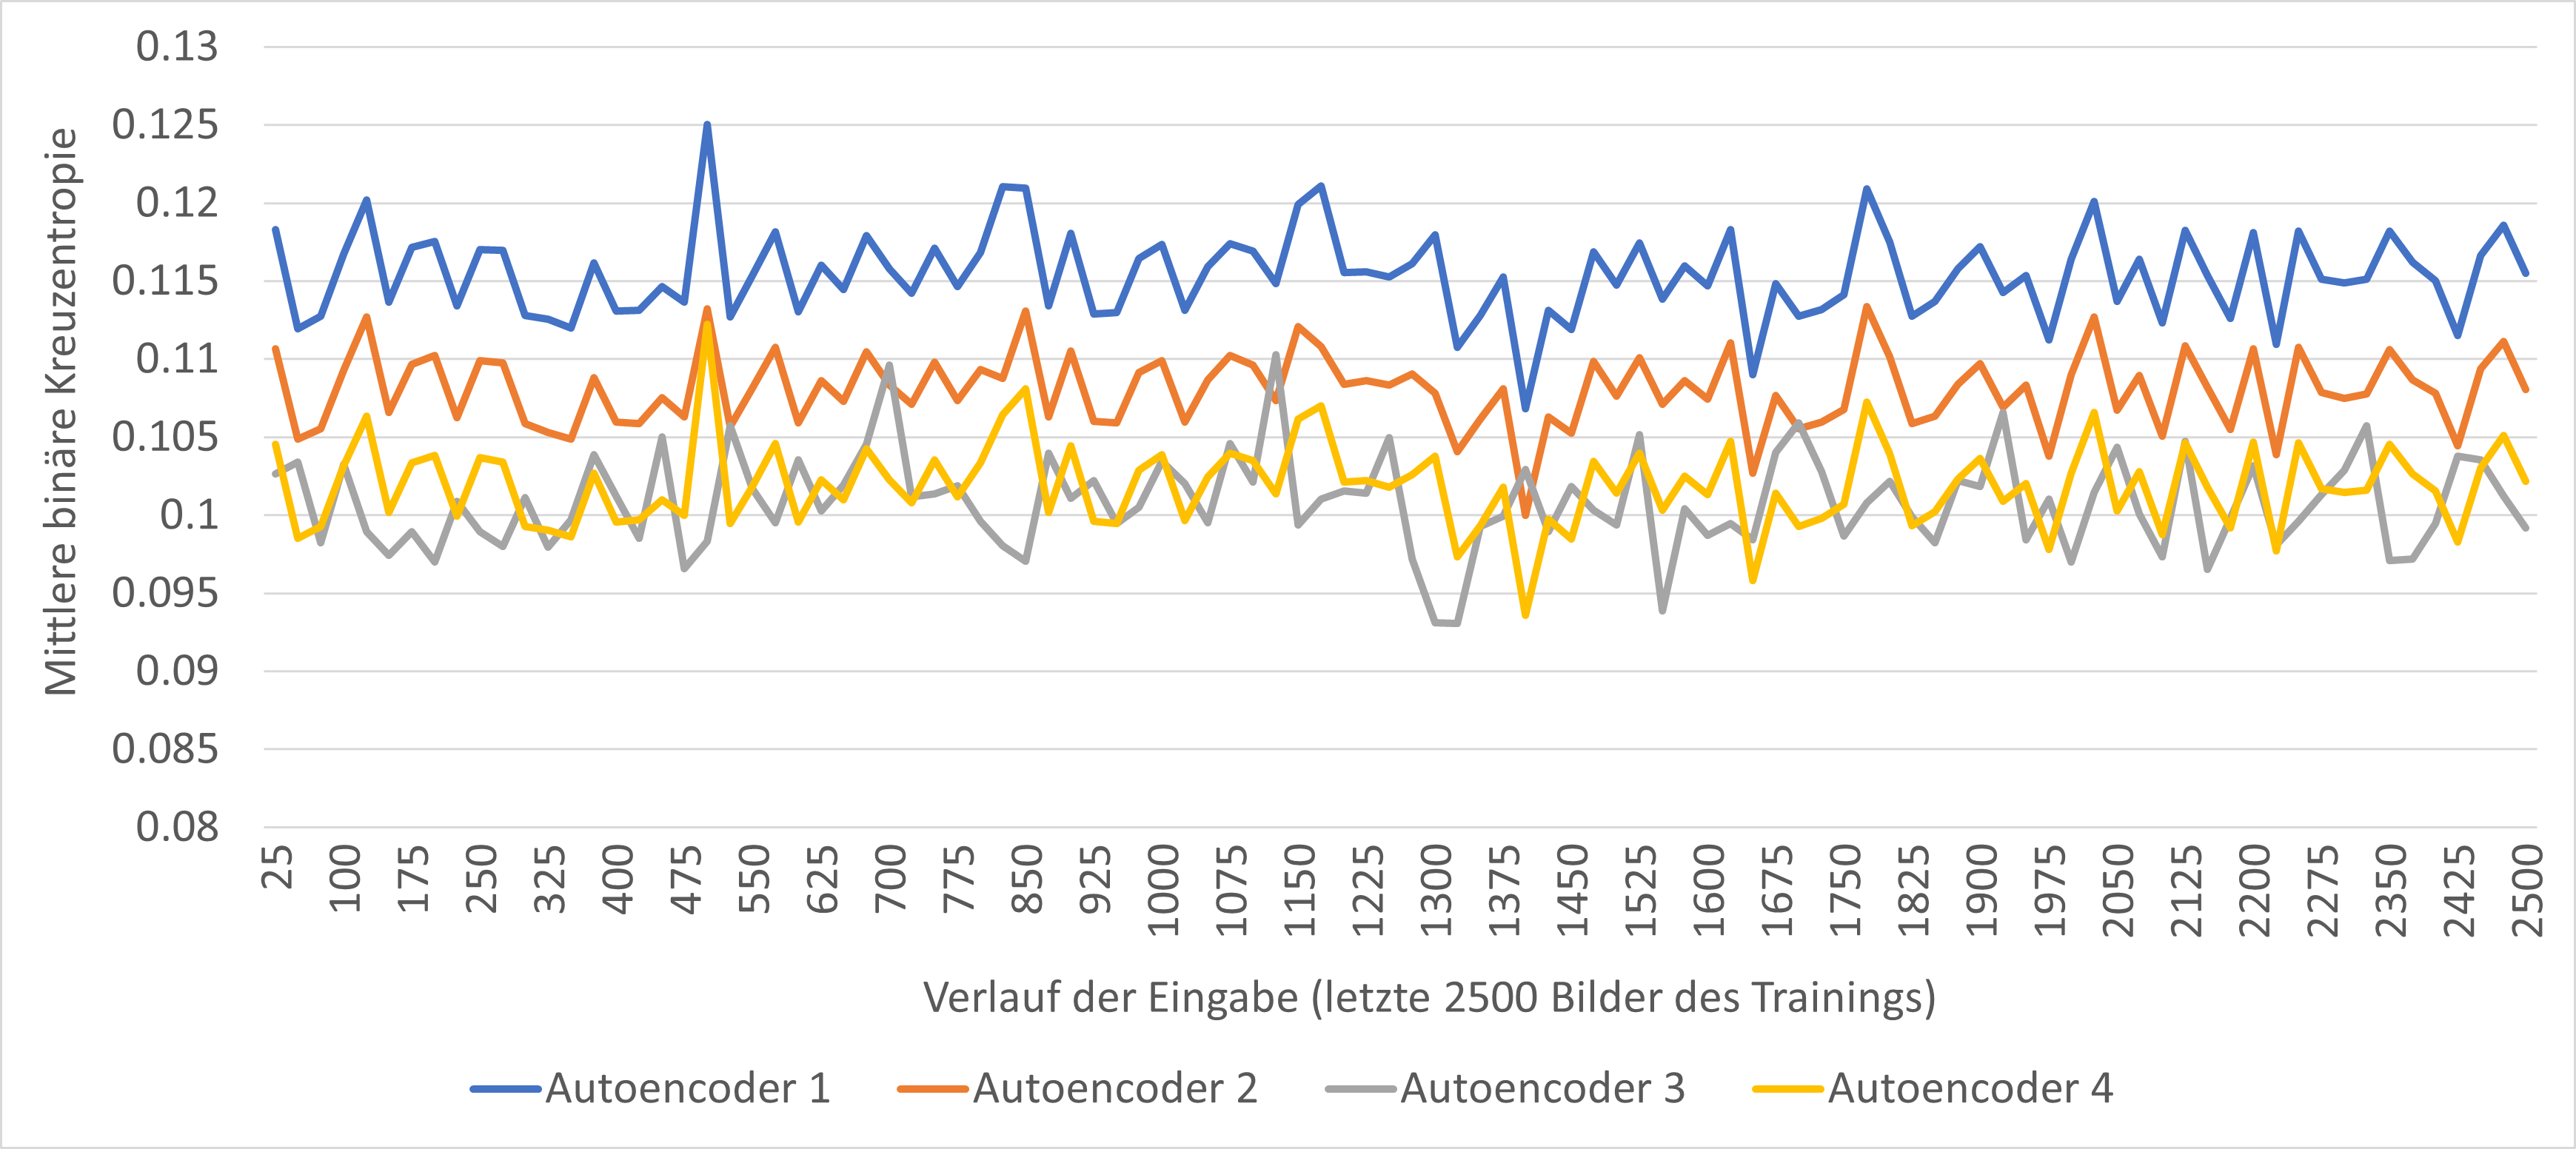
\includegraphics[width=\textwidth]{bilder/training_diagram_last2500.png}
    \caption{Über 300 bzw. 400 Eingaben gemittelte binäre Kreuzentropie der 2500 letzten Batches jedes Autoencoders während des Trainings}
    \label{fig:training_loss_2500}
\end{figure}

\section{Experimente}
Die Autoencoder wurden nach den oben beschriebenen Kriterien trainiert und auf verschiedene Arten und Weisen untersucht. Hierzu wurden mehrere Experimente durchgeführt, in welchen die Generalisierfähigkeit der Autoencoder auf dem Testdatensatz, gegenüber der realen JADX-Applikation sowie gegenüber anderen \glspl{gui} untersucht wurde.

\subsection{Experiment 1 -- MSE auf Testdatensatz}
\label{subsec:exp1}

Das erste durchgeführte Experiment war eine Messung der Qualität der Rekonstruktionen der verschiedenen Autoencoder auf den Testdaten. Hierzu wurden der komplette Testdatensatz als Eingabe für die Autoencoder verwendet und die Ausgaben generiert. Anschließend wurde die Abweichung zwischen Eingabe und Ausgabe mit dem \gls{mse} berechnet und über alle Bilder gemittelt.

\subsubsection*{Ergebnisse}

Die Ergebnisse der Autoencoder-Architekturen unterscheiden sich dabei deutlich und werden in Tabelle~\ref{tab:exp1results} dargestellt.
Autoencoder~\ref{a3} und \ref{a4} schneiden hier am besten ab, während Autoencoder~\ref{a1} und \ref{a2} vergleichsweise schlechte Werte erzielen. So betragen die Mittelwerte des \gls{mse} mehr als das Doppelte des Wertes des Autoencoders~\ref{a3}.


\begin{table}[htbp]
    \centering
    \caption{Ergebnisse der Autoencoder bei Eingabe des Testdatensatzes }
    \label{tab:exp1results}
    \smallskip
    \begin{tabular}{ llll }
        \toprule
        Architektur & Mittelwert des \gls{mse} \\
        \hline
        Autoencoder 1 & $0,004295$ \\
        Autoencoder 2 & $0,003450$ \\
        Autoencoder 3 & \textbf{0,001643} \\
        Autoencoder 4 & $0,001785$ \\
        \bottomrule
    \end{tabular}
\end{table}


\subsubsection*{Fazit}

Ein Unterschied zwischen der Architektur von Autoencoder~\ref{a1} und den anderen Autoencodern liegt in der Verwendung der ReLU-Aktivierungsfunktion anstatt der LeakyReLU-Funktion. Obwohl Ergebnisse von Hu et al.~\cite{huImprovingConvolutionalNeural2018} indizieren, dass die Verwendung der LeakyReLU bei Convolutional-Networks die Ergebnisse um 1-2\% verbessern können, lässt sich dadurch nicht der deutlich schlechtere \gls{mse} erklären. Einen größeren Einfluss auf den schlechteren \gls{mse} dürfte das mit 60~Neuronen vergleichsweise kleine Bottleneck von Autoencodern~\ref{a1} haben. Daher kann es nicht so viele Informationen speichern wie die Bottlenecks der anderen Autoencoder. Autoencoder~\ref{a2} schneidet trotz des sehr großen Bottlenecks von 320~Neuronen ebenfalls vergleichsweise schlecht ab. Dies ist ein Indiz dafür, dass Fully-Connected-Schichten die Ergebnisse gegenüber der ausschließlichen Verwendung von Convolutional-Schichten verbessern können. Dieser Eindruck wird durch die Ergebnisse von Autoencoder~\ref{a3} und \ref{a4} bestärkt, in welchen der Anteil an Fully-Connected-Schichten deutlich höher als in Autoencoder~\ref{a1} ist. Darüber hinaus ist das Bottleneck deutlich breiter.

\subsection{Experiment 2 -- Qualitativer Vergleich der Ergebnisse auf Testdaten}
\label{subsec:exp2}


\begin{figure}[htbp]
    \centering
    \resizebox*{!}{.98\textheight}{\input{AusgabenExp2_1.pdf_tex}}
    \caption{Experiment 2: Vergleich des Bild 1 mit den Ausgaben der Autoencoder. Hochauflösende Bilder siehe Abschnitt \ref{sec:appendix:exp2}}
    \label{exp2_image:1}
\end{figure}

\begin{figure}[htbp]
    \centering
    \resizebox*{!}{.98\textheight}{\input{AusgabenExp2_2.pdf_tex}}
    \caption{Experiment 2: Vergleich des Bild 2 mit den Ausgaben der Autoencoder. Hochauflösende Bilder siehe Abschnitt \ref{sec:appendix:exp2_2}}
    \label{exp2_image:2}
\end{figure}

In diesem Experiment wurden die trainierten Autoencoder qualitativ untersucht. Für diese Masterarbeit ist insbesondere wichtig, dass eine Rekonstruktion als Applikation gut bedienbar wäre sowie die einzelnen \gls{gui}-Elemente sichtbar sind. Eine rein quantitative Betrachtung des \gls{mse} reicht daher nicht aus. Die qualitative Analyse wurde so durchgeführt, dass alle Autoencoder 32 zufällig aus den Testdatensatz ausgewählte Bilder als Eingabe bekamen. Zur Darstellung in dieser Arbeit wurden davon zwei beispielhafte Bilder ausgewählt, anhand welcher die Ergebnisse sowie die Vor- und Nachteile der verschiedenen Autoencoder erklärt werden. Diese Auswahl erfolgte dabei unter der Prämisse, möglichst viele verschiedene \gls{gui}-Elemente der Anwendung JADX darzustellen, um exemplarisch für den Datensatz stehen zu können. Das erste Bild zeigt die Textsuche von JADX und wird zusammen mit den Ausgaben der Autoencoder und deren \gls{mse} in Abb.~\ref{exp2_image:1} dargestellt. Das zweite Bild und die dazugehörigen Ausgaben der Autoencoder bzw. der \gls{mse} befindet sich in Abb.~\ref{exp2_image:2}.

In Tabelle~\ref{tab:exp2results_mse} werden darüber hinaus der \gls{mse} der Autoencoder-Ausgaben auf dem gesamten Testdatensatz mit dem \gls{mse} der für diesen Abschnitt erstellten Untermenge verglichen. Die Abweichung zwischen dem \gls{mse} des Testdatensatzes und der Untermenge ist jeweils gering und liegt ausschließlich im einstelligen Prozentbereich.

\begin{table}[htbp]
    \centering
    \caption{Mittelwert des MSE der Autoencodern-Ergebnisse bei Eingabe des Testdatensatzes und der Untermenge des Testdatensatzes (32 Bilder)}
    \label{tab:exp2results_mse}
    \smallskip
    \begin{tabular}{ llll }
        \toprule
        Architektur & \gls{mse} Testdatensatz & \gls{mse} Untermenge \\
        \hline
        Autoencoder 1 & $0,004295$ & $0,004139$\\
        Autoencoder 2 & $0,003450$ & $0,003326$\\
        Autoencoder 3 & \textbf{0,001643} & \textbf{0,001746}\\
        Autoencoder 4 & $0,001785$ & $0,001944$\\
        \bottomrule
    \end{tabular}
\end{table}

\subsubsection*{Ergebnisse}
Die in diesem Abschnitt beschriebenen Ergebnisse beziehen sich auf die komplette Untermenge des Datensatzes, bestehend aus 32 Bildern. Alle beschriebenen Effekte werden in den Abb.~\ref{exp2_image:1} und \ref{exp2_image:2} dargestellt und können dort nachvollzogen werden.

In der Ausgabe von Autoencoder~\ref{a1} sind alle \gls{gui}-Elemente erkennbar. Über das ganze Bild verteilt befinden sich kleine blaue aber auch schwarze Artefakte -- eine Art Schleier --, womit die Lesbarkeit der Schrift und die Erkennbarkeit von Buttons erschwert ist. Des Weiteren sind deutlich sichtbare Schachbrettmuster erkennbar. Im zweiten Bild wird ersichtlich, dass die blaue, von Windows stammende Kopfleiste nicht klar vom Hintergrund separiert ist und am rechten Rand häufig unvollständig dargestellt wird. Der Button zum Schließen des Fensters wird damit nicht korrekt dargestellt. Ränder von Buttons sind teilweise verwaschen, so in etwa das Feld zur Auswahl des Editor-Themes im Einstellungsfenster von Bild~2. Weiße Buttons auf grauem Hintergrund (sichtbar am unteren Rand des Einstellungsfensters auf Bild~2) sind nicht klar vom Hintergrund abgegrenzt und damit nicht zwangsläufig als Buttons identifizierbar.

Autoencoder~\ref{a2} gibt ein deutlich von Artefakten freieres Bild aus und zeigt darüber hinaus alle \gls{gui}-Elemente klar erkennbar. Die blaue Kopfleiste wird vollständig angezeigt und beinhaltet nur kleine Artefakte. Das Schriftbild ist im Vergleich zu Autoencoder~\ref{a1} zwar freier von Artefakten, dennoch etwas unscharf. Im Vergleich zu Autoencoder~\ref{a1} ist der Kontrast geringer, wodurch das Bild homogener wirkt. Manche Linien erscheinen dennoch nur in einem hellen statt kräftigen Grauton.

Das Ergebnis von Autoencoder~\ref{a3} ist schärfer und kontrastreicher, wodurch das Schriftbild klarer wird. Farbtöne sind insgesamt kräftiger als bei Autoencoder~\ref{a2}, ohne die starken Artefakte von Autoencoder~\ref{a1}. Insbesondere Ränder von Buttons und sonstigen \gls{gui}-Elementen sind vergleichsweise scharf dargestellt. Die blaue Kopfleiste ist sehr trennscharf und einheitlich vom Hintergrund separiert und wird komplett dargestellt. Weiße Buttons auf grauem Hintergrund sind im Vergleich zu Autoencoder~\ref{a1} besser abgegrenzt, jedoch durch die unscharfe Umrandung nicht direkt als Button identifizierbar.

Die Ergebnisse des Autoencoders~4 sind in etwa auf dem Niveau des Autoencoders~3. Im Vergleich sind die Bilder weniger kontrastreich, dafür werden jedoch Flächen etwas gleichmäßiger dargestellt.

Wenn man den \gls{mse} betrachtet, so werden die Ergebnisse aus Experiment~1 aus Abschnitt~\ref{subsec:exp1} hier bestätigt. Autoencoder~\ref{a3} und \ref{a4} schneiden am besten ab, gefolgt von Autoencoder~\ref{a2} und zuletzt Autoencoder~\ref{a1}. Die Werte liegen dabei sehr nah an den Durchschnittswerten aus Experiment 1. Lediglich die Ausgabe von Autoencoder~\ref{a2} weist etwas bessere Werte auf.

\subsubsection*{Fazit}
Autoencoder~\ref{a3} und \ref{a4} schneiden hier am besten ab, da die Bildqualität auf der untersuchten Untermenge des Testdatensatzes besser ist, als bei Autoencoder~\ref{a1} und \ref{a2}. Darüber hinaus liegt der \gls{mse} bei diesen deutlich niedriger. Autoencoder~\ref{a3} und \ref{a4} sind dabei auf ähnlichem Niveau, wobei Autoencoder~\ref{a3} kontrastreichere Bilder ausgibt und Autoencoder~\ref{a4} Flächen etwas homogener darstellt. Der \gls{mse} ist bei Autoencoder~\ref{a3} am geringsten. Autoencoder~\ref{a1} fällt gegenüber den anderen Autoencodern durch die schlechtere Bildqualität und die deutlich sichtbaren Schachbrettmuster ab.

\subsection{Experiment 3 -- Verwendung von Daten der Anwendung JADX}
\label{subsec:exp3}
Ein wichtiger Aspekt in der Bewertung von Autoencoder-Architekturen ist die Fähigkeit zur Generalisierung. In diesem Kontext bedeutet dies nicht nur, den Fehler auf Trainings- und Testdaten zu minimieren, sondern auch auf Daten der realen Applikation. Die Autoencoder sollen letztendlich mit echten \gls{gui}-Daten arbeiten. Daher ist es wichtig zu analysieren, wie gut sie auf echten Daten funktionieren. Insbesondere ist hier wichtig, wie schwer die in Abschnitt~\ref{sec:mock_limitations} besprochenen Unterschiede zwischen Mock und realer \gls{gui} wiegen.

\begin{figure}[htbp]
    \centering
    \resizebox*{!}{.98\textheight}{\input{AusgabenExp3_1.pdf_tex}}
    \caption{Experiment 3: Vergleich des Bild 1 mit den Ausgaben der Autoencoder. Hochauflösende Bilder siehe Abschnitt \ref{sec:appendix:exp3}}
    \label{exp3_image:1}
\end{figure}

\begin{figure}[htbp]
    \centering
    \resizebox*{!}{.98\textheight}{\input{AusgabenExp3_2.pdf_tex}}
    \caption{Experiment 3: Vergleich des Bild 2 mit den Ausgaben der Autoencoder. Hochauflösende Bilder siehe Abschnitt \ref{sec:appendix:exp3_2}}
    \label{exp3_image:2}
\end{figure}


Um diese Fragestellungen zu untersuchen, wurden 22 Abbilder von JADX untersucht. Von diesen werden hier zwei Bilder zusammen mit den Ausgaben der Autoencoder dargestellt. Die 22 Abbilder wurden so ausgewählt, dass sie möglichst viele Facetten von JADX zeigen sollen. Darin enthalten sind sowohl Elemente, die im Mock abgebildet werden, wie die Hauptansicht oder die Textsuche, aber auch Elemente, die nur in der realen JADX-Applikation existieren. Dazu gehören bspw. die Dialoge, um Daten zu öffnen, oder das JADX-Log anzuzeigen. Genaueres zu den Unterschieden der Hauptansicht wird in Abschnitt~\ref{sec:mock_limitations} erklärt. Das erste, hier dargestellte Bild enthält die Hauptansicht von JADX. Die meisten Elemente dieser Ansicht wurden so direkt im Mock, auf welchem die Autoencoder trainiert wurden, abgebildet. Dennoch existieren hier auch Unterschiede, wie die Speicherverbrauchsanzeige am unteren Bildrand, die nicht im Mock implementiert ist. Diese ist daher nicht in den Trainingsdaten vorhanden und stellt für die Autoencoder ein komplett neues Element dar.

Das zweite Bild beinhaltet eine Ansicht, die im entwickelten Mock der \gls{gui} so nicht existiert: das Fenster um Dateien zu öffnen. Dieses wird nur unter Windows so dargestellt, wie abgebildet. Es orientiert sich an der Windows zugrundeliegenden Designsprache. Deshalb ist es der Designsprache von JADX unter Windows, und damit des Mocks, ähnlich.

Die Bilder wurden als Eingabe für jeden Autoencoder verwendet und analysiert. Dabei wurde jeweils der \gls{mse} berechnet und die Bilder einer qualitativen Analyse unterzogen. Die zwei ausgewählten Eingabebilder und die Ergebnisse der Autoencoder zusammen mit dem berechneten \gls{mse} werden in Abb.~\ref{exp3_image:1} und \ref{exp3_image:2} dargestellt.
Ein Vergleich des \gls{mse} des kompletten Datensatzes mit dem \gls{mse} des Testdatensatzes befindet sich in Tab.~\ref{tab:exp3results_mse}.

\begin{table}[htbp]
    \centering
    \caption{Mittelwert des MSE der Autoencoder-Ausgaben bei Eingabe des Testdatensatzes und der Bilder der JADX-Applikation (22 Bilder)}
    \label{tab:exp3results_mse}
    \smallskip
    \begin{tabular}{ llll }
        \toprule
        Architektur & \gls{mse} Testdatensatz & \gls{mse} Datensatz JADX \\
        \hline
        Autoencoder 1 & $0,004295$ & $0,011156$\\
        Autoencoder 2 & $0,003450$ & $0,010440$\\
        Autoencoder 3 & \textbf{0,001643} & $0,009843$\\
        Autoencoder 4 & $0,001785$ & \textbf{0,009283}\\
        \bottomrule
    \end{tabular}
\end{table}

\pagebreak
\subsubsection*{Ergebnisse}
Die Resultate des 2. Experimentes aus Abschnitt \ref{subsec:exp2} lassen sich weitgehend auf alle hier untersuchten Bilder übertragen. Insbesondere die im vorigen Experiment aufgetretenen Artefakte bei Autoencoder~\ref{a1}, die leichte Unschärfe und Kontrastarmut bei Autoencoder~\ref{a2} und die bessere Darstellung von Flächen durch Autoencoder~\ref{a4} sind auch hier auffällig.

Im Besonderen wird die Hauptansicht (sichtbar in Abb.~\ref{exp3_image:1}) von allen Autoencodern so rekonstruiert, dass der Projektbaum in der linken Bildhälfte und der Editor in der rechten Bildhälfte erkennbar bleiben. Größere Unterschiede treten bei den Elementen auf, die nicht im Mock vorkommen. Die grüne Leiste als Teil der Speicherverbrauchsanzeige wird bei Autoencoder~\ref{a1} nur extrem schwach oder gar nicht angezeigt. Die textuelle Repräsentation des Speicherverbrauchs ist zwar in Andeutungen erkennbar, aber unlesbar. Autoencoder~\ref{a2} zeigt zwar die Leiste der Speicherverbrauchsanzeige an, wenn auch teilweise in einer verfälschten Farbe. Der Text ist jedoch ebenfalls größtenteils unlesbar. Autoencoder~\ref{a3} und \ref{a4} können die Leiste zwar darstellen, allerdings ist diese bei den Ausgaben beider Autoencoder auf den meisten Bildern des Datensatzes unvollständig. Bei Autoencoder~\ref{a4} wird die Farbe der Leiste korrekt wiedergegeben. Der dazugehörige Text ist sowohl bei Autoencoder~\ref{a3} als auch bei Autoencoder~\ref{a4} unscharf, aber lesbar.

Ein weiteres, nur in der realen JADX-Applikation vorkommendes Element ist die über der Speicherverbrauchsanzeige liegende Tab-Navigation. Mit dieser kann zwischen Java-Code und der Smali-Notation (einer Art Java-VM-Assembler) gewechselt werden. Diese wird von den Autoencodern~\ref{a3} und \ref{a4} am besten dargestellt. Hier ist sowohl erkennbar, dass es sich um Buttons handelt, als auch, welcher Tab ausgewählt ist. Die übrigen Autoencoder stellen zwar den Text dar, die Buttons sind jedoch nicht oder nur schlecht als solche identifizierbar. Die Balken rund um den Editor und den Projektbaum, über die eine Scrollfunktion implementiert ist, werden von Autoencoder~\ref{a3} und \ref{a4} dargestellt. Autoencoder~\ref{a1} stellt lediglich einen der Balken korrekt dar, während in den Ausgaben des Autoencoders~\ref{a2} kein Balken sichtbar ist.

Neben den Elementen, die nicht im Mock vorkommen, gibt es auch bei der Darstellung des Menüs und der Icon-Leiste am oberen Bildrand Unterschiede zwischen den einzelnen Autoencodern. Lediglich Autoencoder~\ref{a4} stellt beides in einer solchen Qualität dar, dass alle Elemente erkennbar sind. Bei den Autoencodern~\ref{a1} und \ref{a2} sind sowohl der Text als auch die Icons teilweise nur schwach sichtbar. Autoencoder~\ref{a3} gibt den Text und die Icons stärker aus. Über dem linken oberen Eck des Bildes liegt jedoch bei einigen Bildern (erkennbar in Abb.~\ref{exp3_image:1}) eine Art großflächige Störung vor, welche den Text und die Icons teilweise unlesbar macht. Diese tritt vor allem bei Auswahl des Hauptfensters von JADX auf, wodurch sich die Windows-Kopfleiste blau färbt. Lediglich die Ergebnisse von Autoencoder~\ref{a4} sind so geartet, dass der Text lesbar ist und die Mehrzahl der Icons gut identifizierbar bleibt.

Zusätzliche Fenster, bspw. das in Abb.~\ref{exp3_image:2} dargestellte Fenster zum Öffnen einer Datei, werden von allen Autoencodern so dargestellt, dass der Inhalt lesbar und die Icons identifizierbar sind. Die Darstellungsqualität der einzelnen Elemente schwankt jedoch deutlich, sodass Autoencoder~\ref{a1} die bekannten Artefakte insbesondere bei Flächen und Icons aufweist und Autoencoder~\ref{a2} die Schrift und die Icons eher schwach darstellt. Die Ausgabe der Autoencoder~\ref{a3} und \ref{a4} enthält die Elemente in besserer Darstellungsqualität, wobei die Icons kontrastarm angezeigt werden. Insbesondere Ränder um Buttons und Eingabefelder werden hier scharf dargestellt. Eingefärbte Flächen, bspw. gelb-markierte Code-Bereiche wie in Abb.~\ref{exp3_image:1}, werden von Autoencoder~\ref{a3} und \ref{a4} teilweise blau anstatt in der Ursprungsfarbe eingefärbt. Eine Erklärungsmöglichkeit hierfür liegt darin, dass Autoencoder diese Bereiche womöglich als blaue Windows-Kopfleiste einstufen, weshalb eine Farbverwechslung erfolgt.

Wenn man den \gls{mse} betrachtet, so werden die großen Abstände in den Ergebnissen aus Experiment~1 des Abschnittes~\ref{subsec:exp1} hier deutlich kleiner. Auffällig ist, dass Autoencoder~\ref{a4} in diesem Experiment einen niedrigeren \gls{mse} erreicht als Autoencoder~\ref{a3}. Autoencoder~\ref{a4} erreicht nach dem \gls{mse} bei 18 von 22 Bildern ein besseres Ergebnis als Autoencoder~\ref{a3}. Dieser Abstand wird bei den Bildern, in welchen bei Autoencoder~\ref{a3} die Störung aus Bild~1 auftritt, deutlicher. Der Wert von Autoencoder~\ref{a3} liegt dort näher bei den Werten der Autoencoder~\ref{a1} und \ref{a2}.


\subsubsection*{Fazit}
Autoencoder~\ref{a4} schneidet in diesem Experiment sowohl bzgl. des \gls{mse} als auch in der qualitativen Analyse am besten ab, da er das Originalbild am besten rekonstruieren kann. Bei einigen Bildern, wie Bild 1, liegt der Wert des Autoencoders~\ref{a4} deutlich vor den weiteren Autoencodern, während bei Bild~2 Autoencoder~\ref{a3} und \ref{a4} auf einem ähnlichen Niveau abschneiden.

Die Frage nach den besten Fähigkeiten zur Generalisierung kann -- jedenfalls im Rahmen dieses Experiments -- Autoencoder~\ref{a4} für sich entscheiden. Dieser konnte am besten mit den Unterschieden zwischen dem Mock und JADX umgehen. Die Elemente, die nicht im Mock enthalten sind, werden von Autoencoder~\ref{a4} am genauesten dargestellt. Bei diesem Autoencoder treten auch die wenigsten Bildstörungen auf.

\subsection{Experiment 4 -- Verwendung von weiteren GUIs}
\label{subsec:exp4}

Der nächste Schritt in der Generalisierung besteht darin, \glspl{gui} als Eingabe für die Autoencoder zu verwenden, auf denen kein Training stattfand. Die zugrundeliegende Fragestellung ist die, ob ein Autoencoder so entwickelt werden kann, dass er für ganze Familien von Anwendungen geeignet ist. Um diese Fragestellungen stichprobenhaft zu untersuchen, wurden zwei Abbilder von Anwendungen als Eingabe für die Autoencoder verwendet. Das erste Bild zeigt den Windows Explorer. Dieser wurde ausgewählt, da er eine vollständig unterschiedliche Anwendung darstellt, im Kern jedoch einer ähnlichen Designsprache folgt. Der Windows Explorer ist strukturell ähnlich zu JADX aufgebaut: Einem zweispaltiges Layout bestehend aus einer Baumstruktur in der linken Spalte sowie zeilenweisen Einträgen in der rechten Spalte. Das Farbschema ist dem von JADX ähnlich und besteht hauptsächlich aus Weiß- und Grautönen sowie dem Blauton der Windows-Kopfleiste. Darüber hinaus ist der Inhalt -- genau wie bei JADX -- sehr textlastig und wird durch die häufige Verwendung kleiner Icons unterstützt.

Das zweite, verwendete Bild ist ein Screenshot der Webseite des Repositories dieser Masterarbeit auf GitHub\footnote{\url{https://github.com/research-manuscripts/MA_Felix_Rittler}, letzter Zugriff: 13.11.2021} (Stand: 13.11.2021). Im Vergleich zu JADX und dem Windows Explorer kommt hier eine völlig andere Designsprache zum Einsatz. Erstens ist der \emph{Dark Mode} von GitHub aktiviert, sodass das Bild durch einen höheren Anteil sehr dunkler Bereiche geprägt ist. Darüber hinaus unterscheiden sich verwendeten Farben deutlich.

Beide Bilder wurden, wie im vorigen Experiment, als Eingabe für die Autoencoder verwendet. Die Ausgaben und der dazugehörige \gls{mse} werden in Abb.~\ref{exp4_image:1} und \ref{exp4_image:2} dargestellt.

\begin{figure}[htbp]
    \centering
    \resizebox*{!}{.98\textheight}{\input{AusgabenExp3_3.pdf_tex}}
    \caption{Experiment 4: Vergleich des Bild 1 mit den Ausgaben der Autoencoder. Hochauflösende Bilder siehe Abschnitt \ref{sec:appendix:exp4}}
    \label{exp4_image:1}
\end{figure}

\begin{figure}[htbp]
    \centering
    \resizebox*{!}{.98\textheight}{\input{AusgabenExp3_4.pdf_tex}}
    \caption{Experiment 4: Vergleich des Bild 2 mit den Ausgaben der Autoencoder. Hochauflösende Bilder siehe Abschnitt \ref{sec:appendix:exp4_2}}
    \label{exp4_image:2}
\end{figure}

\subsubsection*{Ergebnisse}
Autoencoder~\ref{a3} und \ref{a4} können das Bild des Windows Explorers in besserer Qualität anzeigen als Autoencoder~\ref{a1} und \ref{a2}. Die Defizite bzgl. Störungen und der Darstellung der blauen Kopfleiste treten hier wie in Experiment~3 in Abschnitt~\ref{subsec:exp3} auf. Autoencoder~\ref{a2} verursacht diese zwar nicht, gibt das Bild aber insgesamt kontrastarm wieder. Einige Icons, aber auch Text, werden sehr hell dargestellt, wodurch die Erkennbarkeit und Lesbarkeit erschwert werden. Bei Autoencoder~\ref{a3} ist die Lesbarkeit deutlich besser, jedoch tritt hier wieder die aus Experiment~\ref{subsec:exp3} bekannte Bildstörung in der oberen linken Bildecke auf. Autoencoder~\ref{a4} schafft es, alle Bildelemente am besten darzustellen. Der Kontrast ist vor allem gegenüber Autoencoder~\ref{a2} -- aber bei Icons auch gegenüber Autoencoder \ref{a3} -- höher, ohne, dass dabei Bildstörungen entstehen. Der Text ist bei der Ausgabe von Autoencoder~\ref{a4} sehr gut lesbar, wobei ihm dies am unteren Bildrand besser gelingt als Autoencoder~\ref{a3}.

Der gemessene \gls{mse} bestätigt die Ergebnisse. Während Autoencoder~\ref{a2} bis \ref{a3} auf ähnlichem Niveau im Bereich zwischen $0,0074$ und $0,0078$ liegen, liegt Autoencoder~\ref{a4} mit $0,0058$ deutlich darunter. Autoencoder~\ref{a1} weist mit $0,0085$ eindeutig den schlechtesten Wert auf.

Das Bild der Webseite wird von allen Autoencodern stark verfälscht rekonstruiert. Kein Autoencoder stellt die Farbe der Webseite dar, lediglich bei Autoencoder~\ref{a1} sind immerhin Teile in einer verfälschten Farbe eingefärbt. Der Text ist nur bei Autoencoder~\ref{a2} in Ansätzen erkennbar. Autoencoder~\ref{a3} und \ref{a4} stellen lediglich die Flächen, auf denen sich im Originalbild Inhalt befindet, korrekt dar. Der Inhalt ist jedoch nicht les- oder erkennbar. Betrachtet man die zum Webbrowser gehörenden \gls{gui}-Elemente, verändert sich das Bild etwas. Hier schneiden wie bei allen Bildern zuvor Autoencoder~\ref{a3} und \ref{a4} am besten ab. So stellen diese die Icons gut erkennbar dar. Auch Autoencoder~\ref{a2} zeigt die Icons, wobei die Unschärfe zunimmt. Die Flächen werden durch Autoencoder~\ref{a2} und \ref{a4} am besten dargestellt. Das von Autoencoder~\ref{a1} ausgegebene Bild weist die bereits beobachteten Artefakte auf und zeigt einige Icons nur sehr schwach. Die Lesbarkeit der Schrift ist an dieser Stelle ebenso nicht gegeben.
Der gemessene \gls{mse} ist bei allen Autoencodern sehr hoch und ist nahe bei $0,5$. Diesbezüglich schneidet kein Autoencoder deutlich besser oder schlechter ab.

\subsubsection*{Fazit}
Die Ausgaben der Autoencoder zu Bild~1 sind in ihrer Qualität vergleichbar zu den Ergebnissen, die diese bei Eingabe der realen JADX Applikation in Experiment~3 erreichen. Dies wird durch den gemessenen \gls{mse} untermauert, bei dem alle Autoencoder bei Bild~1 sogar besser abschneiden, als bei Bild~1 aus Experiment~2. Es ist auch hier so, dass Autoencoder~\ref{a4} die besten Ergebnisse erzielt.
Der Wert von Autoencoder~\ref{a3} wird besonders von dem gestörten Bildbereich negativ beeinflusst.

Die Ergebnisse ändern sich bei Bild~2 jedoch deutlich. Kein Autoencoder schafft es, die Webseite in akzeptabler Qualität darzustellen. Eine Erklärungsmöglichkeit ist in dem vollständig anderen Farbschema der Webseite zu finden. Alle anderen Eingaben für die Autoencoder (Testdaten, JADX und der Windows Explorer) sind in ihrer Designsprache vergleichsweise ähnlich und bestehen überwiegend aus hellen Flächen mit kleinen Icons und schwarzem Text. Die Webseite ist jedoch sehr dunkel. Für diesen Erklärungsansatz spricht, dass die Kopfleiste des Webbrowsers deutlich besser dargestellt wird und deren Rekonstruktion qualitativ näher an den Rekonstruktionen der Autoencoder aus den anderen Experimenten ist.

Auch wenn die Ergebnisse dieses Experiments durch die Datenmenge in Gestalt einer kleinen Stichprobe nur eine eingeschränkte Aussagekraft haben, lassen sich hier die Grenzen der Autoencoder aufzeigen. So kann man zum einen ableiten, dass sich prinzipiell auch auf anderen Applikationen als jener, mit der das Training stattfand, gute Ergebnisse erzielen lassen. Die Rekonstruktion der Ansichten unter Verwendung komplett unterschiedlicher Farbschemata ist jedoch komplexer und mit den hier entwickelten Autoencodern und den derzeitigen Trainingsdaten nicht möglich.

\subsection{Experiment 5 -- Geschwindigkeit}
\label{subsec:exp5}
Nicht zuletzt ist auch die Geschwindigkeit der Autoencoder ein wichtiger Parameter, um diese zu bewerten. Im Zusammenhang mit neuronalen Netzen wird in der Regel die Inferenzzeit zur Bewertung verwendet. Die Inferenzzeit bezeichnet die benötigte Zeit, um aus einer Eingabe eine Vorhersage zu berechnen. Nicht Teil dieser Zeit sind insbesondere die Vorgänge, um Daten auf die \gls{gpu} zu verschieben, zur Initialisierung der Netze und Parameter und der Aufwärmvorgang der \gls{gpu}. Die Inferenzzeit wurde für alle Autoencoder sowohl unter Verwendung der \gls{gpu} als auch der \gls{cpu} berechnet.

Als Host-Rechner wurde eine Workstation des \gls{fzi} verwendet, deren Spezifikationen in Tab.~\ref{tab:workstation} dargestellt werden. Das Modul \texttt{torch.distributed}, das es ermöglicht, mehrere \glspl{cpu} einzubeziehen, blieb bei der Messung der Inferenzzeit außen vor. Daher fanden die Berechnungen immer nur auf einer \gls{cpu} statt.

In diesem Experiment wurde ein zufälliger Eingabevektor 300 mal als Eingabe verwendet und die Inferenzzeiten, wie im vorigen Abschnitt beschrieben, gemessen. Aus den gemessenen 300 Inferenzzeiten wurde der Mittelwert und die Standardabweichung berechnet. Diese Messungen und Berechnungen wurden dabei für jeden der 4 Autoencoder jeweils auf der \gls{cpu} und auf der \gls{gpu} durchgeführt.

\pagebreak
Zusätzlich zu Mittelwert und Standardabweichung wird jeweils noch ein sog. \gls{gpu}-Beschleunigungsfaktor $s$ angegeben.
Dieser beschreibt die mittlere Beschleunigung durch Verwendung der \gls{gpu} statt der \gls{cpu} und wird wie folgt aus dem Mittelwert der Inferenzzeiten auf der \gls{cpu} $\overline{x}_{CPU}$ und dem Mittelwert der Inferenzzeiten auf der \gls{gpu} $\overline{x}_{GPU}$ berechnet:

\begin{equation}
    s = \frac{\overline{x}_{CPU}}{\overline{x}_{GPU}}
\end{equation}

\begin{table}[t]
    \centering
    \caption{Spezifikationen der verwendeten Workstation}
    \label{tab:workstation}
    \smallskip
    \begin{tabularx}{8.3cm}{ lX }
        \toprule
        Komponente & Modell \\
        \hline
        CPU & 2 x Intel Xeon Gold 6258R \\
        CPU-Architektur & Intel Cascade Lake \\
        CPU-Kerne & jew. 28 Kerne à 2,7 GHz mit max. 56 Threads \\
        GPU & Nvidia Tesla V100S 32 GB \\
        Grafikchip & Nvidia Volta GV100 \\
        Arbeitsspeicher & 256 GB \\
        \bottomrule
    \end{tabularx}
\end{table}

\subsubsection*{Ergebnisse und Fazit}
Die Ergebnisse der Messungen und der \gls{gpu}-Beschleunigungsfaktor werden in Tab.~\ref{tab:exp5results} dargestellt. Autoencoder~\ref{a2} erzielt dabei in allen Kategorien die besten Ergebnisse. Dieser gibt sowohl auf der \gls{cpu} als auch auf der \gls{gpu} am schnellsten ein Ergebnis aus. Daneben ist bei diesem Autoencoder der Vorteil bei der Verwendung der \gls{gpu} mit einem Faktor von $55,93$ am höchsten. Autoencoder~\ref{a3} und \ref{a4} erreichen fast identische Werte mit leichten Vorteilen für Autoencoder~\ref{a4}, wohingegen Autoencoder~\ref{a1} vergleichsweise langsam ist. Letzterer besitzt zusätzlich eine deutlich geringere Beschleunigung bei Verwendung der \gls{gpu}.

Über alle Autoencoder hinweg stehen die Inferenzzeiten in Korrelation zur Größe der ersten Convolutional-Schicht. Die vergleichsweise hohe Inferenzzeit des Autoencoders~\ref{a1} lässt sich durch die aufwendigen Berechnungen in der ersten Schicht mit einem 32x32-Filter erklären. Autoencoder~\ref{a2} weißt mit Abstand die geringste Inferenzzeit auf -- eine Tatsache, die sich durch die geringe Filtergröße der ersten Convolutional-Schicht, aber auch durch die fehlenden Fully-Connected-Schichten, erklären lässt. Insbesondere Autoencoder~\ref{a3} und \ref{a4} weisen besonders große Fully-Connected-Schichten auf.

\begin{table}[htbp]
    \centering
    \caption{Mittelwert und Standardabweichung der Inferenzzeit bei Verwendung der CPU bzw. GPU der Workstation und GPU-Beschleunigungsfaktor}
    \label{tab:exp5results}
    \smallskip
    \begin{tabular}{ llllll }
        \toprule
        \multirow{2}{*}{Architektur} & \multicolumn{2}{c}{CPU} & \multicolumn{2}{c}{GPU} & GPU- \\
        \cline{2-5}
        & Mittelwert & Std & Mittelwert & Std & Beschleunigung $s$ \\
        \hline
        Autoencoder 1 & $4,1731s$ & $0,1219$ & $0,2830s$ & $0,0053949$ & $14,75$\\
        Autoencoder 2 & \textbf{0,6779s} & 0,0147 & \textbf{0,0121s} & $0,0005165$ & \textbf{55,93}\\
        Autoencoder 3 & $1,5976s$ & $0,0427$ & $0,0404s$ & $0,0003145$ & $39,58$\\
        Autoencoder 4 & $1,5061s$ & $0,0325$ & $0,0389s$ & $0,0003203$ & $38,67$\\
        \bottomrule
    \end{tabular}
\end{table}

\section{Erfahrungen und Fehlschläge}
Neben den hier vorgestellten Autoencodern~\ref{a1} bis \ref{a4} mit guten Ergebnisse, wurden auch Architekturen entwickelt, die keine guten oder teilweise auch sehr schlechte Ergebnisse erzielten. Diese Ansätze, welche im Rahmen dieser Masterarbeit nicht funktionierten, sollen in diesem Abschnitt dargestellt werden. Es wird hier die Zielsetzung verfolgt, zukünftigen Entwicklern und Forschern weitere Erfahrungen und Anhaltspunkte auf den Weg zu geben. Mit diesen Erfahrungen soll es einfacher werden, bessere Autoencoder zu entwickeln, ohne die gleichen Fehler erneut zu begehen. In diesem Abschnitt werden daher zudem Vermutungen angestellt, warum diese Ansätze nicht funktionierten.

\begin{figure}[htbp]
    \centering
    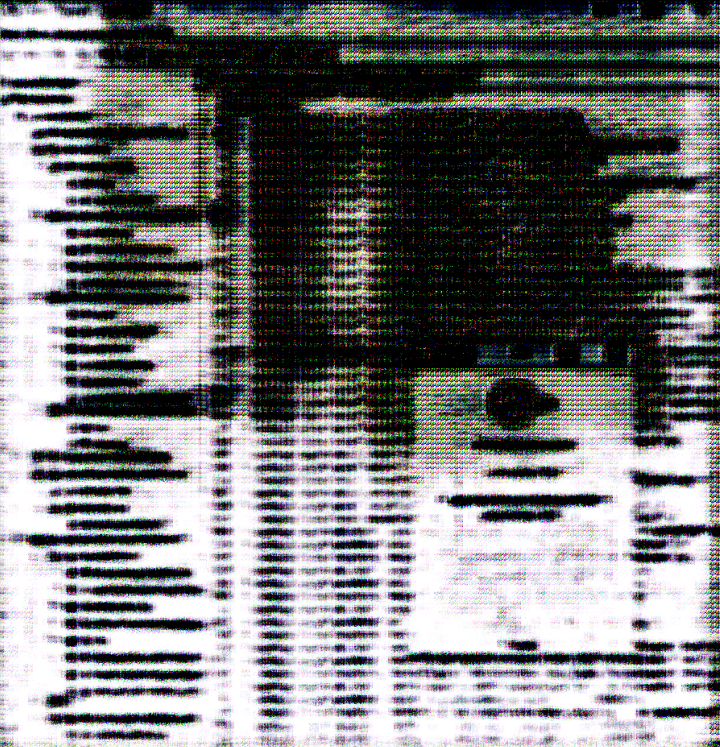
\includegraphics[width=0.6\textwidth]{bilder/image_relu_problems.png}
    \caption{Bildstörungen bei Verwendung der ReLU- und LeakyReLU-Aktivierungsfunktion als letzte Schicht}
    \label{fig:image_relu_problems}
\end{figure}

Während der Entwicklung stellte sich als wichtig heraus, dass die Convolutional-Schichten der Autoencoder über ein ausreichend großes Padding verfügen. Dieses Padding sorgt dafür, dass der Filter einer Convolutional-Schicht nicht an den Rändern der Eingabe beginnt, sondern über die Eingabe hinaus geht. Die Ränder und insbesondere die Ecken der Eingabe werden somit häufiger als Eingabe für die Filter verwendet. Ohne Padding würden beispielsweise die Ecken der Eingabe nur ein einziges Mal als Eingabe für die Filter verwendet, womit diese deutlich unterrepräsentiert wären. Damit ist ein Padding wichtig, um eine über das Bild hinweg gleichmäßig hohe Rekonstruktionsqualität zu erreichen. Insbesondere in der ersten Schicht der Autoencoder, in welcher die Eingabe und die Filter am größten sind, stellte sich die Verwendung eines Paddings als wichtig heraus. Dieses wurde in der Regel genauso groß wie der Filter gewählt. In den weiteren Schichten betrug die Größe des Paddings meist 1.

Darüber hinaus war es wichtig, dass die Aktivierungsfunktionen innerhalb des Decoder-Teils in etwa den Wertebereich [0,1] aufweisen. Es wurden Versuche durchgeführt, die ReLU- sowie die LeakyReLU-Funktion im Decoder-Teil des Autoencoders einzusetzen. Dies führte jedoch zu großflächigen Störungen, wie in Abb.~\ref{fig:image_relu_problems} dargestellt. Hier war zwar die grobe Bildeinteilung noch sichtbar, der Inhalt jedoch nicht mehr erkennbar.

Des Weiteren wurden Versuche unternommen, die Funktion \texttt{torch.BCELossWithLogits}\footnote{\url{https://pytorch.org/docs/stable/generated/torch.nn.BCEWithLogitsLoss.html}, letzter Zugriff: 13.12.2021} als Fehlerfunktion einzusetzen, die die binäre Kreuzentropie mit einer Sigmoid-Schicht verbindet und dadurch eine höhere numerische Stabilität erreicht. Die Ergebnisse waren jedoch schlechter als bei einer Verwendung der reinen binären Kreuzentropie. Dies könnte damit zusammenhängen, dass durch die zusätzliche Sigmoid-Schicht zwei Sigmoid-Funktionen nacheinander zum Einsatz kamen, da die letzte Schicht der Autoencoder ebenso die Sigmoid-Funktion beinhaltet. Dieser Zusammenhang kann in Zukunft genauer untersucht werden.

Daneben ist zu beachten, dass der Filter einer Convolutional-Schicht nicht deutlich kleiner ist, als das anschließend durchgeführte Pooling.
Hieraus resultierten Schachbrettmuster und eine schlechtere Bildqualität. Der Hintergrund für diese Beobachtung könnte sein, dass Pooling-Vorgänge nicht überlappend sind. Wenn der Filter der vorherigen Convolutional-Schicht nun sehr klein ist, werden Informationen über Bildbereiche hinweg, die größer sind als der Filter aber kleiner als die durch das Pooling zusammengefassten Bildbereiche, unter Umständen während der Faltung nicht erkannt und beim Pooling verworfen.



% \chapter{Evaluierung}
% Nachdem die Implementierungsarbeiten abgeschlossen sind, werden einige Experimente und Messungen durchgeführt. Im Vordergrund steht hierbei die Evaluierung der Autoencoder-Architekturen, d.h. wie gut diese jeweils abschneiden und wo die Stärken und Schwächen liegen. Darüber hinaus findet auch eine allgemeine Evaluierung der Stärken und Schwächen von Autoencodern im konkreten Anwendungsfall statt. Die Experimente zielen auf die Beantwortung der in der Masterarbeit zu beantwortenden Forschungsfragen, wie sie in der GQM-Analyse in Abschnitt NO GQM beschrieben werden.
% \todo{proposal wg GQM referenzieren?}
% Die Experimente laufen dabei so ab, dass Autoencoder mit generierten Daten trainiert werden. Anschließend werden mehrere Metriken berechnet, aus denen sich bestimmte Schlüsse hinsichtlich der Forschungsfrage ableiten lassen. Im oben genannten Abschnitt über die GQM-Analyse werden zu jeder zentralen Forschungsfrage die Metriken beschrieben, die die Experimente charakterisieren.
% % \begin{itemize}
% %     \item Was für Experimente werden durchgeführt?
% %     \item Was ist wichtig?
% %     \begin{itemize}
% %         \item Performance
% %         \item Welche Autoencoder können gut (=gute Ergebnisse) vom am FZI entwickelten CTRNN verwendet werden?
% %     \end{itemize}
% % \end{itemize}

\chapter{Diskussion}
Nachdem sowohl der \gls{gui}-Mock entwickelt wurde, die Autoencoder entworfen und untersucht und die Ergebnisse einzeln analysiert wurden, folgt in diesem Kapitel die Gegenüberstellung und ein experimentübergreifender Vergleich der einzelnen Architekturen. Anschließend werden die experimentellen Ergebnisse verwendet, um die Qualität des Datensatzes zu beurteilen sowie die Qualität des Datensatzgenerators zu diskutieren.

\section{Autoencoder}
Wenn man die Autoencoder gegenüberstellen und vergleichen will, ist zu unterscheiden in Fähigkeiten, Trainings- und Testdaten zu erlernen, sowie Fähigkeiten zur Generalisierung. Ersteres wird in Experiment~1 in Abschnitt~\ref{subsec:exp1} analysiert, in welchem Autoencoder~\ref{a3} knapp vor Autoencoder~\ref{a4} am besten abschneidet. Diese Ergebnisse werden durch Experiment~2 aus Abschnitt~\ref{subsec:exp2} bestätigt -- sowohl in der qualitativen Analyse als auch bei Betrachtung des \gls{mse} der Bilder der Untermenge des Testdatensatzes. Die Autoencoder~\ref{a1} und \ref{a2} schneiden deutlich schlechter ab -- sowohl wenn man den \gls{mse} betrachtet als auch in den qualitativen Analysen. Eine Erklärungsmöglichkeit hierfür kann darin liegen, dass die Fully-Connected-Schichten des Autoencoders~\ref{a1} mit einer Bottleneck-Größe von 60 Neuronen zu klein dimensioniert ist. Der besonders große Filter mit 32x32 bringt jedenfalls im Rahmen dieser Architektur keinen so großen Vorteil, als dass die Ergebnisse auf ähnlichem Niveau wie der anderen Autoencoder liegen würden.

% Wie können Autoencoder GUI Infos lernen
Die Frage nach den besten Fähigkeiten zu Generalisierung lässt sich nicht so einfach beantworten. Auch in den Experimenten, in denen Abbilder von JADX und des Windows Explorers als Eingabe verwendet werden, schneiden Autoencoder~\ref{a1} und \ref{a2} schlechter ab Autoencoder~\ref{a3} und \ref{a4}. Die Abstände in der Ergebnisqualität der Autoencoder sind jedoch deutlich geringer als auf dem Testdatensatz. Ist der Mittelwert des \gls{mse} bei Autoencoder~\ref{a4} auf dem Testdatensatz aus Abschnitt~\ref{subsec:exp1} noch $58\%$ geringer als bei Autoencoder~\ref{a1}, so schrumpft diese Differenz auf dem aus JADX-Bildern bestehenden Datensatz auf $20\%$. Selbst die absolute Differenz der Werte von Autoencoder~\ref{a1} und \ref{a4} sinkt von einem Wert von $0,00251$ auf $0,00187$, obwohl der \gls{mse} auf den Vorhersagen bei den Bildern der echten JADX-Applikation gegenüber dem Testdatensatz deutlich ansteigt.
Auffällig ist jedoch die Beobachtung, dass der Autoencoder~\ref{a4} auf der realen JADX-Applikation bessere Ergebnisse erzielt. Dies liegt zu einem großen Teil an einer Störung in der oberen linken Bildecke, die bei Autoencoder~\ref{a3} auftritt. Die Fähigkeit zur Generalisierung scheint bei Autoencoder~\ref{a4} daher ausgeprägter. Wenn man die Architekturen betrachtet, scheint das deutlich größere Bottleneck von 360 Neuronen bei Autoencoder~\ref{a3} entweder keinen großen Vorteil zu bieten, oder die Vorteile werden durch die Verwendung der LeakyReLU-Aktivierungsfunktion im Decoder-Teil negativ ausgeglichen. Der Rest der Architektur ist identisch.

Die Antwort auf die Frage, welcher Autoencoder am besten generalisieren kann, ist eine Frage des Blickwinkels. Wenn nur die Ergebnisse der Experimente betrachtet werden, die auf Fähigkeiten zur Generalisierung testen sollen, dann ist dies Autoencoder~\ref{a4}. Wenn man jedoch die Ergebnisse auf den Testdaten mit einbezieht, dann kommen die Qualitäten, die Autoencoder~\ref{a4} auf den Testdaten besonders auszeichnen, auf den generelleren Daten nicht so zur Geltung. Das gelernte Wissen von Autoencoder~\ref{a1} und \ref{a2} scheint daher ebenso sehr genereller Natur zu sein.

Eine Gemeinsamkeit aller Autoencoder ist, dass sie nur vergleichsweise schlecht mit dunklen Flächen und komplett verschiedenen Designsprachen umgehen können. Dies wird jedenfalls durch die Ergebnisse von Experiment~4 in Abschnitt~\ref{subsec:exp4} angedeutet. Wenn man dieses Ergebnis mit den Ergebnissen der weiteren Experimente kombiniert, liegt der Schluss nahe, dass es weniger auf die Anwendung selbst ankommt, deren Ansichten komprimiert wird. Viel mehr sind die Designsprache und die verwendeten Farben wichtig.

% Wie können Autoencodern GUI Info reduzieren
Autoencoder~\ref{a2} weißt ein vergleichsweise großes Bottleneck von 320 Neuronen auf. Dennoch erzielt dieser Autoencoder sowohl bei Betrachtungen der \gls{mse} als auch in den qualitativen Analysen schlechtere Ergebnisse als Autoencoder~\ref{a3} und \ref{a4} mit ähnlich großem bzw. sogar kleinerem Bottleneck. Der mit Abstand größte Unterschied zwischen Autoencoder~\ref{a3} bzw. \ref{a4} und Autoencoder~\ref{a2} ist das Fehlen von Fully-Connected-Schichten bei Autoencoder~\ref{a2}. Diese Tatsache in Kombination mit dem experimentellen Ergebnis bestärkt die Erkenntnis, die bereits Kies~\cite{kiesEntwicklungUndAnalyse2020} in ihrer Arbeit gewann, dass ein gewisser Anteil an Fully-Connected-Schichten die Ergebnisse verbessern kann.
Der Einsatz von Autoencoder~\ref{a2} kann dennoch sinnvoll sein, falls eine niedrige Inferenzzeit nötig ist. Wie in Abschnitt~\ref{subsec:exp5} gezeigt wurde, ist diese bei Autoencoder~\ref{a2} 3-4 mal niedriger als bei den Autoencodern~\ref{a3} und \ref{a4}. Autoencoder~\ref{a2} komprimiert zwar durch seine vergleichsweise große Bottleneck-Größe schwächer, ist dabei aber sehr effizient.   Autoencoder~\ref{a1} schneidet zwar sowohl hinsichtlich der Geschwindigkeit als auch der Qualität der Ergebnisse am schlechtesten ab, zeigt jedoch seinen Vorteil durch ein sehr kleines Bottleneck. Wenn eine sehr starke Kompression nötig ist, kann selbst dieser Autoencoder seine Stärken ausspielen. Um die vergleichsweise hohe Inferenzzeit zu verringern, könnte als Maßnahme die Verkleinerung des Filters der Größe 32x32 überlegt werden. Die Ergebnisse der anderen Autoencoder legen nahe, dass auch mit geringerer Filtergröße eine qualitativ hochwertige Kompression erreicht werden kann und auch komplexe Features, wie etwa einzelne Buchstaben und Text, gelernt werden können.

Im Gegensatz zu den zuvor dargestellten Autoencodern gibt es im aktuellen Entwicklungsstand keinen ersichtlichen Grund, Autoencoder~\ref{a3} einzusetzen. Obwohl dessen Bottleneck größer ist, als das von Autoencoders~\ref{a4}, erreicht er keine wesentlich besseren Ergebnisse, sondern schneidet teilweise sogar schlechter ab. Darüber hinaus benötigt dieser vergleichsweise viel Speicher, wodurch sich die Trainingsdauer durch die notwendige Verringerung der Batchgröße verlängert. Auch ohne Beachtung des Speicherverbrauchs ist die Inferenzzeit leicht größer als die von Autoencoder~\ref{a4}. Durch den Austausch der LeakyReLU-Aktivierungsfunktionen durch Sigmoid-Funktionen könnte sich eine Verbesserung der Ergebnisse ergeben, wodurch Autoencoder~\ref{a3} wieder eine valide Option wird. Wenn sich keine Verbesserung der Ergebnisse einstellen sollte, würde dies bedeuten, dass in dieser Autoencoder-Architektur eine Vergrößerung des Bottlenecks über 180 Neuronen zu keinem signifikanten Vorteil führt. Damit wäre in jedem Szenario Autoencoder~\ref{a4} die bessere Wahl.

% \begin{itemize}
%     \item Reine Testergebnisse
%     \item Generalisierung
%     \item Ergebnisse auf JADX
%     \item Geschwindigkeit vs Qualität
%     \item
% \end{itemize}
% \begin{itemize}
%     \item In experimentelle Ergebnisse Relation setzen
%     \item Autoencoder einstufen: Stärken und Schwächen
%     \item Erklärungsmöglichkeiten aufschreiben
%     \item Beobachtung: A3 auf Trainingsdaten besser, A4 generalisiert aber besser. (A3 generalisiert vglw schlecht, teilweise nur auf Niveau von A2)
%     \item A1 am schlechtesten (Nicht gut, langsam und generalisiert nicht gut)
%     \item Stärke von A2: Performance!
%     \item Empfehlung: Bei hoher Performance A2, sonst A4. A4 benötigt mehr Speicher.
%     \item A3 benötigt ZU VIEL Speicher bei nicht besseren Ergebnissen (eher schlechter)
%     \item Unterschiedliche Hyperparameter entkräften
% \end{itemize}


\section{Datensatzqualität}
% Die Bewertung der Qualität des Datensatzes ist im Zusammenhang mit dem in dieser Masterarbeit untersuchten Ansatz sehr wichtig, da der Datensatz-Generator einer der wichtigsten Bausteine dieses Ansatzes ist.

Insgesamt betrachtet, kann die Qualität des Datensatzes als sehr gut beurteilt werden. Bei neuronalen Netzen gilt es insbesondere komplexe Randfälle ausreichend abzudecken. Dies bedeutet im vorliegenden Fall auch \gls{gui}-Elemente und Ansichten abzudecken, die weniger häufig auftreten. Die Ergebnisse von Experiment 2 aus Abschnitt~\ref{subsec:exp2} zeigen, dass die \gls{gui}-Elemente aus den Trainingsdaten gleichmäßig gut durch die Autoencoder rekonstruiert werden. Dies lässt den Schluss einer ausreichenden Abdeckung der Randfälle zu.

Einige Fenster, wie die Einstellungen, werden von Nutzern seltener aufgerufen als andere Fenster. Üblicherweise legt ein Nutzer zu Beginn der Nutzung Einstellungen fest und verändert diese danach länger nicht mehr. Der Unterschied zwischen dem hier verwendeten Datensatz und realitätsnahen Datensätzen wäre, dass tiefer versteckte Fenster wie die Einstellungen nicht so häufig in den Daten vorhanden wären. Die Qualität der Rekonstruktion wäre unter Umständen schlechter gewesen.

%Einen Aspekt, den man hier noch einbeziehen kann, ist die Fähigkeit zur Generalisierung. Die Ergebnisse der Experimente~\ref{subsec:exp3} und \ref{subsec:exp4} zeigen, dass die Autoencoder gut generalisieren können, solange ähnliche Designsprachen und Farbschemata verwendet werden. Daher ist vorstellbar, dass die Autoencoder diese Fähigkeiten auch auf \gls{gui}-Elementen, die weniger häufig im Datensatz vorkommen, angewandt werden können. Gute Fähigkeiten zur Generalisierung können daher helfen, gute Ergebnisse auf \gls{gui}-Elementen zu erreichen, die weniger häufig in den Daten vorkommen. Diese Annahme geht jedoch davon aus, dass sich die Fähigkeiten zur Generalisierung nicht verändern, wenn der Datensatz weniger ausgewogen oder nach anderen Kriterien gestaltet wird. Dies ist in dieser Pauschalität nicht belegt und unwahrscheinlich.

\section{Qualität des Generators}
Ein Ziel dieser Masterarbeit war die Untersuchung, wie die Generierung von Trainingsdaten funktionieren muss, um Autoencoder und die neuronalen Netze am \gls{fzi} trainieren zu können. Neben der bereits im vorigen Abschnitt durchgeführten Bewertung der Qualität des generierten Datensatzes, gehört dazu, die Einfachheit in der Handhabung des Generators selbst zu bewerten.

Auch wenn die Qualität des Datensatzes sehr gut ist, ist der Generator dennoch lediglich eingeschränkt einsetzbar. Die Generierung von Datensätzen funktioniert, sie ist jedoch nur über ein Bash-Skript ausführbar. Darüber hinaus ist ein Zugriff auf die Abbilder der \gls{gui} nicht per Offscreen Buffer möglich. Stattdessen muss die Mock-Applikation auf dem Host-PC geöffnet und ein Screenshot erstellt werden. Dies ist fehleranfällig, da nicht überprüft werden kann, ob die Mock-Applikation schon vollständig geladen ist. Der aktuelle Ansatz sieht vor, eine hartkodierte Zeitspanne abzuwarten, bevor der Screenshot erstellt wird. Darüber hinaus ist dieses Vorgehen vergleichsweise langsam, da es mehrere hundert Millisekunden dauert bis ein Betriebssystemfenster mit geladener Anwendung geöffnet ist. Eine Idee war es zudem, die Resultate des Generators \emph{live} als Eingabe für die Autoencoder oder die am \gls{fzi} entwickelten Netze zu verwenden. Die Autoencoder sind jedoch, bei Ausführung auf der \gls{gpu}, alle deutlich schneller als der Datensatzgenerator.

Hinzu kommen die weiteren Limitierungen des verwendeten Frameworks aus Abschnitt~\ref{sec:mock_limitations}: Dies betrifft unter anderem Fehler des Layout-Systems und Darstellungsprobleme bei Inhalt in zusätzlichen Fenstern. Der hier verwendete Ansatz ist daher zum aktuellen Zeitpunkt nicht dauerhaft und produktiv einsetzbar.

% \begin{itemize}
%     \item Wie können Autoencoder GUI Infos lernen
%     \item Wie können Autoencodern GUI Info reduzieren
%     \item Wie muss die Generierung funnktonieren damit Autoencoder gut trainiert werden können?
%     \item Hohe Ausführungsgeschwindigkeit
%     \item Wie eignet sich Rust?
% \end{itemize}




\chapter{Fazit und Ausblick}
Ein Fazit zu dieser Masterarbeit lässt sich zu beiden Zielen ziehen. Einerseits zum Ansatz des Trainingsdatengenerators, mit welchem die für diese Arbeit notwendigen Daten generiert wurden und der dafür gedacht war die am \gls{fzi} entwickelten Netze zu trainieren. Andererseits zu den Autoencodern, die die hochdimensionalen Eingabedaten in Form von Bildern der \gls{gui} komprimieren sollen.

% \subsubsection*{Fazit}

Ein Generator, wie er hier entwickelt wurde, bietet einige Vorteile. Zunächst können Trainingsdaten so generiert werden, wie sie gerade benötigt werden. Die Wahrscheinlichkeitsverteilung des Generators konnte komplett an die Notwendigkeiten der Autoencoder angepasst werden. Dadurch ist es möglich die einzelnen Bestandteile der \gls{gui} so zu gewichten, dass alle Elemente und Komponenten gleichmäßig gut durch die Autoencoder erlernt werden. Jeder Randfall kann im Generator so gewichtet werden, dass der Autoencoder diesen Randfall erkennen und erlernen kann. Darüber hinaus kann so die aufwendige Erhebung und unter Umständen komplexe Vorverarbeitung von Datensätzen der realen Welt vermieden werden.

Gleichzeitig sind die hier verwendeten \gls{gui}-Frameworks der Programmiersprache Rust noch nicht so weit, als dass sie sich in diesem Kontext produktiv einsetzen lassen. Bugs und fehlende Features wie das Offscreen Rendering machen einen Einsatz als Trainingsdatengenerator kompliziert. Der Ansatz, dass Trainingsdaten spontan generiert werden, um neuronale Netze zu trainieren, ist aufgrund der schlechten Performance und der umständlichen Handhabung nicht möglich.

% \subsection*{Autoencoder}

Ein positiveres Fazit lässt sich bezüglich der Autoencoder-Architekturen ziehen. Diese schaffen es, eine komplexe \gls{gui} -- wie die von JADX -- auf 60 bis 180 Neuronen zu komprimieren und dabei qualitativ hochwertige Ergebnisse zu erzielen. Dies gilt sowohl bei Betrachtung des \gls{mse} als auch bezüglich der qualitativen Analyse. Dabei kommen unterschiedliche Stärken und Schwächen zum Vorschein. Insbesondere Autoencoder~\ref{a4} schafft es, starke Kompression mit sehr guten Ergebnissen und einer akzeptablen Geschwindigkeit zu verbinden. Wenn eine höhere Geschwindigkeit benötigt wird oder der für Autoencoder~\ref{a4} nötige Grafikspeicher nicht zur Verfügung steht, liefert Autoencoder~\ref{a2} ähnlich gute Ergebnisse bei etwas schwächerer Kompression auf 320 Neuronen. Wenn umgekehrt eine besonders starke Kompression der Eingabe notwendig ist, kann Autoencoder~\ref{a1} die Eingabe immer noch in akzeptabler Qualität reproduzieren.

Ein wichtiges Fazit in der Arbeit von Kies~\cite{kiesEntwicklungUndAnalyse2020} war, dass der \gls{mse} nur eine geringe Aussagekraft über die tatsächliche Qualität einer Autoencoder-Architektur hat. Diese These kann in dieser Arbeit nicht bestätigt werden. Der \gls{mse} korreliert bei allen Experimenten und Autoencodern mit den Ergebnissen der qualitativen Analyse. Dies könnte mit den gegenüber der Arbeit von Kies veränderten Daten zusammenhängen. Bei Kies waren Farbänderungen von Flächen ein wichtiger Teil der Information in der \gls{gui}, während dies hier nicht der Fall ist. Veränderungen ergeben sich über den Inhalt in Form von Text.

Wie gut die Ergebnisse der einzelnen Autoencoder im Zusammenspiel mit den am \gls{fzi} entwickelten Netzen sind, kann zukünftig noch evaluiert werden. In diesem Kontext ist insbesondere interessant, welche Autoencoder-Kodierungen von den am \gls{fzi} entwickelten Netzen besonders gut verarbeitet werden können. Eine gute und effiziente Kodierung im Bottleneck muss nicht zwangsläufig gut geeignet für die am \gls{fzi} entwickelten Netze sein. Für diesen Zweck wird nur der Encoder-Teil der Autoencoder benötigt. Wenn ein Autoencoder eine Eingabe besonders gut und effizient kodiert, die Rekonstruktion des Decoders jedoch scheitert, wird dieser in hier durchgeführten Untersuchungen dennoch schlecht abschneiden. Nur im Kontext mit den am \gls{fzi} entwickelten Netzen kann daher der Encoder isoliert untersucht werden.

Eine Untersuchung, wie gut die verschiedenen Autoencoder auf anderen Datensätzen abschneiden, könnte Gegenstand weiterer Fragestellungen sein. Die Ergebnisse aus Experiment 3 und 4 sind dahingehend vielversprechend, da sie zeigen, dass die Autoencoder auch auf ganz anderen Anwendungen gut abschneiden können (und nicht nur auf den Trainings- und Testdaten). Die Ergebnisse legen nahe, dass eine Generalisierung auf Anwendungen mit ähnlichen Designsprachen und Farbschemata sehr gut funktioniert. Im Rahmen dieser Masterarbeit wurde an dieser Stelle nur eine kleine Stichprobe analysiert, sodass hier noch weitere Untersuchungen nötig sind. Dies bezieht sich insbesondere auf die Frage, bei welchem Grad an Abweichungen zwischen Trainingsdaten und letztendlicher Eingabe die Ergebnisse eines Autoencoders schlechter werden.

Der Ansatz bzgl. des Trainingsdatengenerators hat hier in Teilen gut funktioniert, die Schwächen der konkreten Umsetzung sind jedoch offensichtlich. Die Programmiersprache Rust und darin entwickelte \gls{gui}-Toolkits weisen noch nicht den nötigen Reifegrad auf. Der Einsatz eines solchen Generators bleibt weiterhin interessant. Die Realisierung durch andere Technologien ist dabei zu prüfen. Einen reinen Trainingsdatengenerator ließe sich auch mit geringerem Aufwand über Webtechnologien realisieren. Alternativ könnte man untersuchen, ob es für C oder C++ Technologien gibt, die die Anforderungen besser erfüllen als die Frameworks in Rust.

% \begin{itemize}
%     \item Vorteil Generator: Wahrscheinlichkeitsverteilung selbstbestimmt (unabhängig von Nutzung)
% \end{itemize}
% \subsection*{Autoencoder}
% \begin{itemize}
%     \item A4 >= A3 > A2 > A1
%     \item A2 Stärke besonders schnell --> Kann auch sinnvoll sein den einzusetzen
%     \item Auf Kies Fazit eingehen: Deren Fazit war, dass Farbänderungen nicht ausreichend durch MSE berücksichtigt werden
% \end{itemize}

% \subsection*{Ausblick}

% \begin{itemize}
%     % \item Die Fähigkeiten zur Generalisierung auf anderen Datensätzen können daher in zukünftigen Arbeiten untersucht werden.
%     % \item Wichtig: Nur erster Aufschlag! In Experimenten nur sehr sehr wenige Bilder qualitativ untersucht.
%     % \item Besserer Generator mit anderen Mitteln?
%     % \item Wie funktionieren die Autoencoder an den Netzen?
% \end{itemize}
%% --------------------
%% |   Bibliography   |
%% --------------------

%% Add entry to the table of contents for the bibliography
\setlength\emergencystretch{1em}

\printbibliography[heading=bibintoc]

%% ----------------
%% |   Appendix   |
%% ----------------
\appendix
%% LaTeX2e class for student theses
%% sections/appendix.tex
%%
%% Karlsruhe Institute of Technology
%% Institute for Program Structures and Data Organization
%% Chair for Software Design and Quality (SDQ)
%%
%% Dr.-Ing. Erik Burger
%% burger@kit.edu
%%
%% Version 1.3.5, 2020-06-26

\iflanguage{english}
{\chapter{Appendix}}    % english style
{\chapter{Anhang}}      % German style
\label{chap:appendix}


%% -------------------
%% | Example content |
%% -------------------
\section{Resultate Experiment 2}
\label{sec:appendix:exp2}
\begin{figure} [ht]
  \centering
  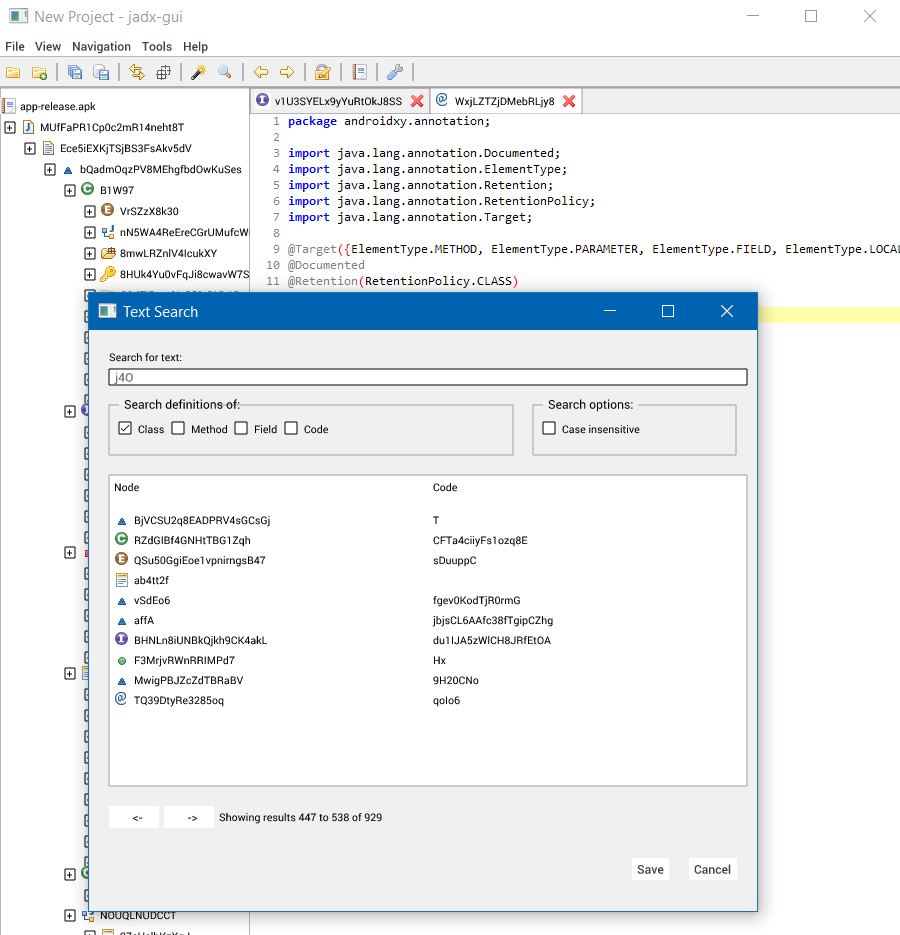
\includegraphics[height=0.67\textheight]{bilder/result_exp2/0.png}
  % 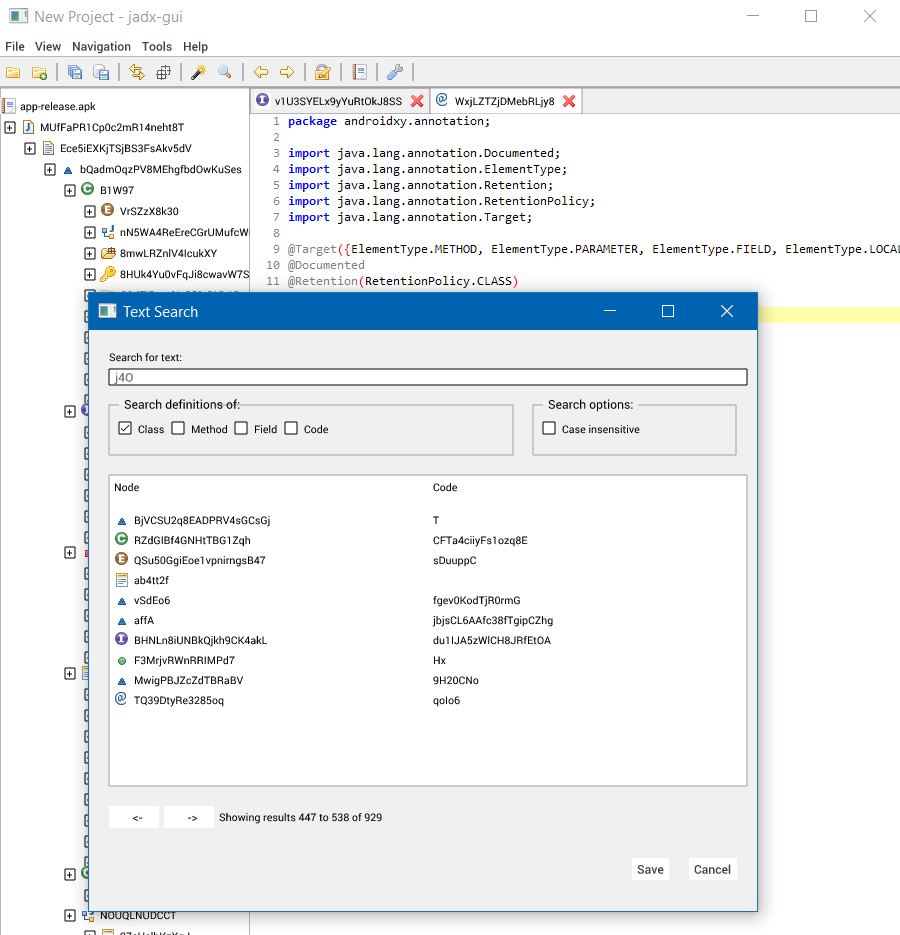
\includegraphics[width=\textwidth]{bilder/result_exp2/0.png}

  \caption{Experiment 2: Originalbild 1 aus Abb.~\ref{exp2_image:1} in hoher Auflösung}
\end{figure}

\begin{figure} [ht]
  \centering
  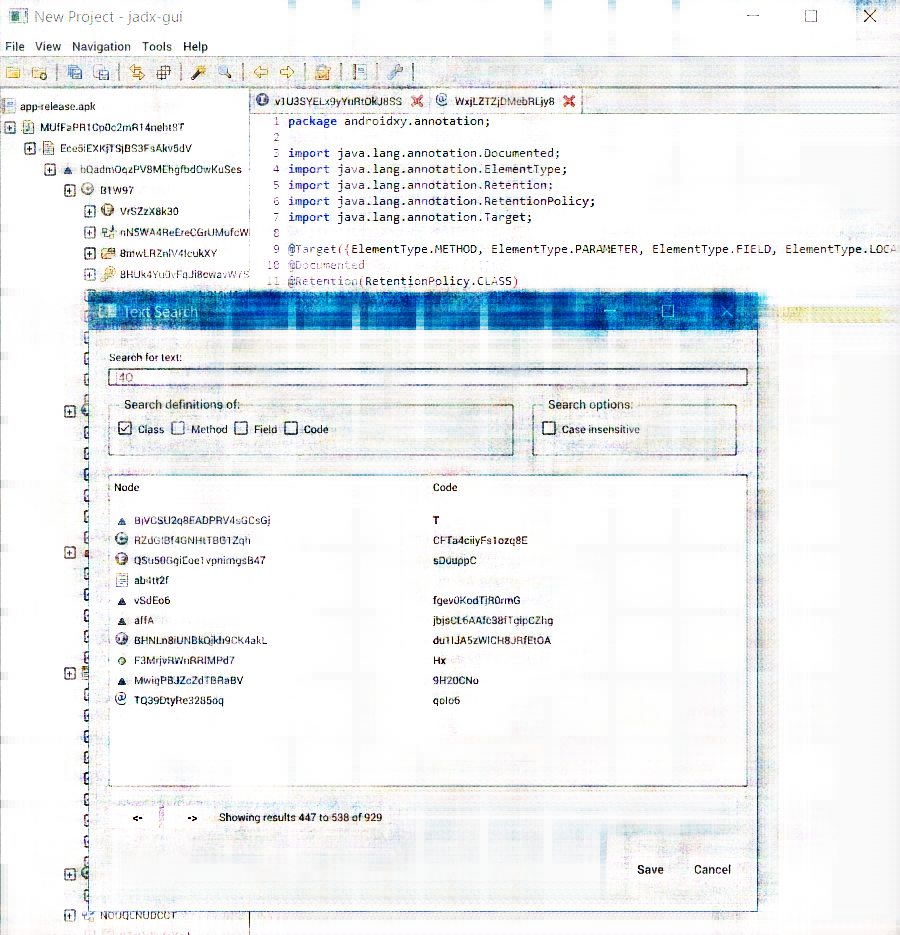
\includegraphics[width=\textwidth]{bilder/result_exp2/0_pred_a1.png}

  \caption{Experiment 2: Ausgabe des Autoencoders~\ref{a1} zu Bild 1 aus Abb.~\ref{exp2_image:1} in hoher Auflösung}
\end{figure}

\begin{figure} [ht]
  \centering
  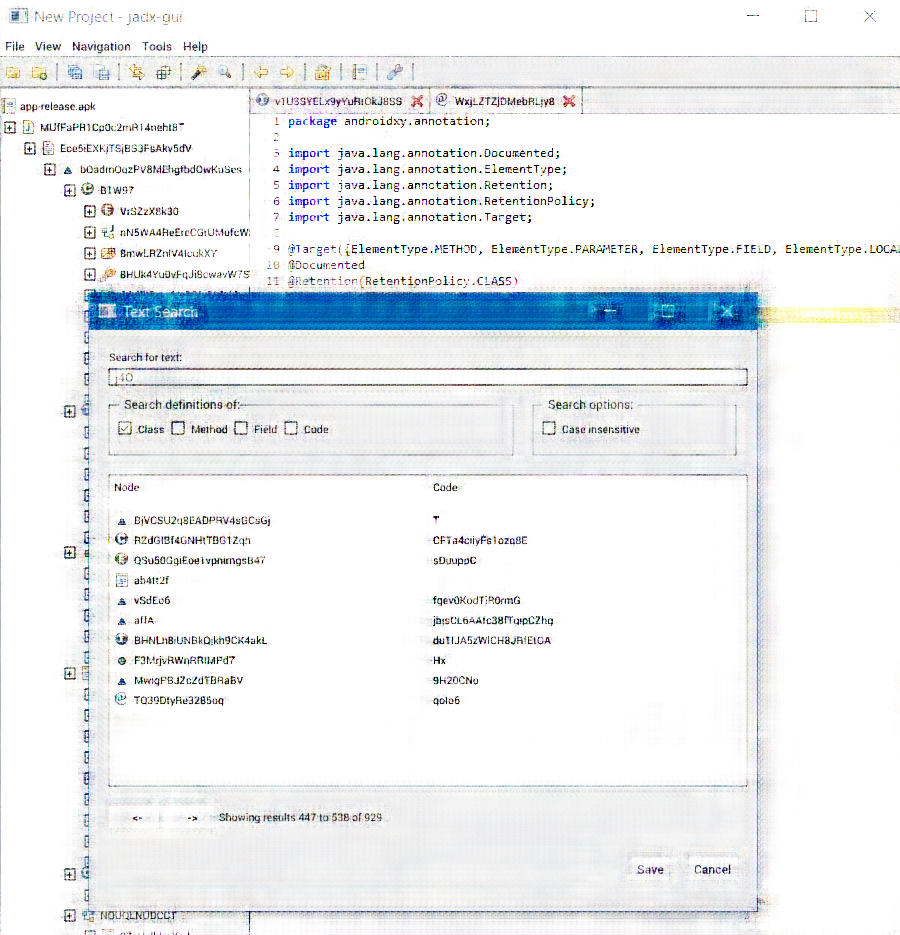
\includegraphics[width=\textwidth]{bilder/result_exp2/0_pred_a2.png}

  \caption{Experiment 2: Ausgabe des Autoencoders~\ref{a2} zu Bild 1 aus Abb.~\ref{exp2_image:1} in hoher Auflösung}
\end{figure}

\begin{figure} [ht]
  \centering
  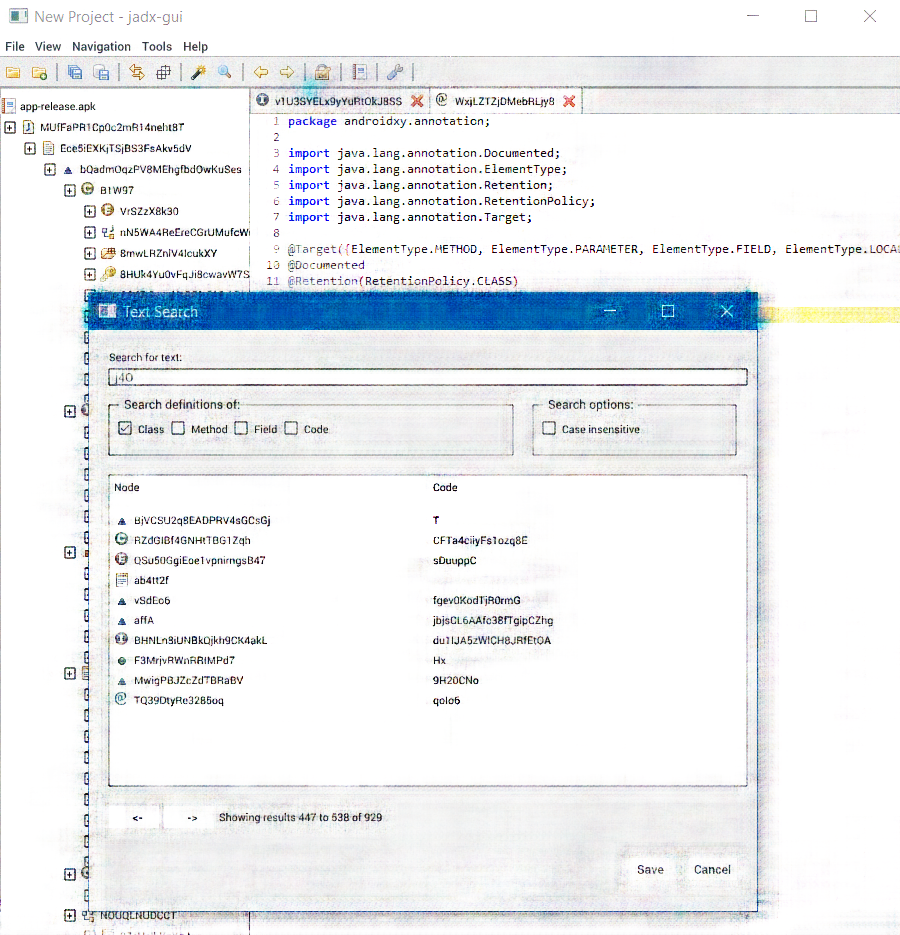
\includegraphics[width=\textwidth]{bilder/result_exp2/0_pred_a3.png}

  \caption{Experiment 2: Ausgabe des Autoencoders~\ref{a3} zu Bild 1 aus Abb.~\ref{exp2_image:1} in hoher Auflösung}
\end{figure}

\begin{figure} [ht]
  \centering
  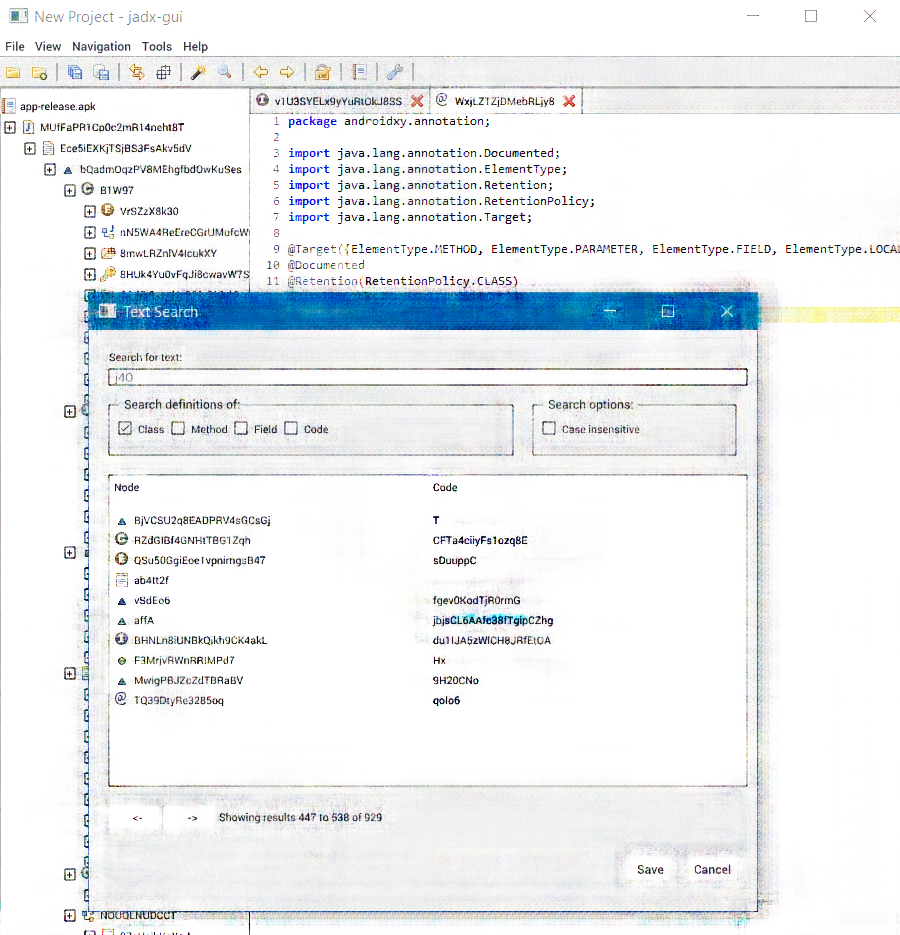
\includegraphics[width=\textwidth]{bilder/result_exp2/0_pred_a4.png}

  \caption{Experiment 2: Ausgabe des Autoencoders~\ref{a4} zu Bild 1 aus Abb.~\ref{exp2_image:1} in hoher Auflösung}
\end{figure}

\label{sec:appendix:exp2_2}
\begin{figure} [ht]
  \centering
  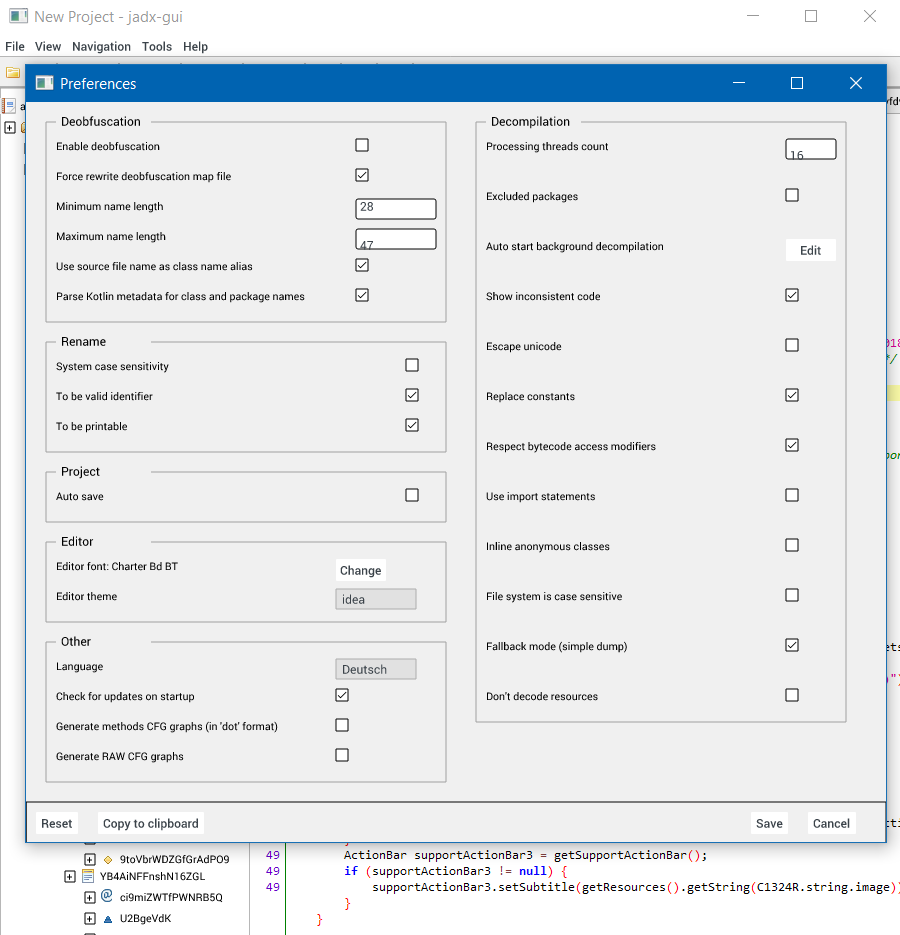
\includegraphics[width=\textwidth]{bilder/result_exp2/1.png}

  \caption{Experiment 2: Originalbild 2 aus Abb.~\ref{exp2_image:2} in hoher Auflösung}
\end{figure}

\begin{figure} [ht]
  \centering
  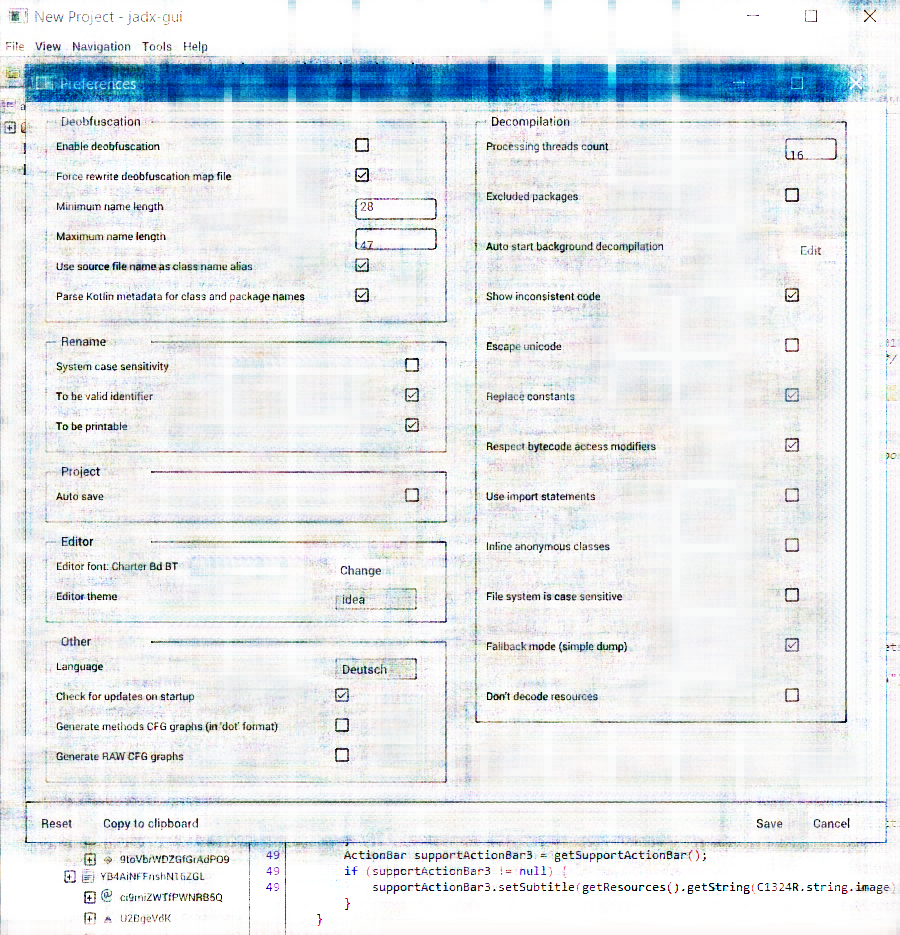
\includegraphics[width=\textwidth]{bilder/result_exp2/1_pred_a1.png}

  \caption{Experiment 2: Ausgabe des Autoencoders~\ref{a1} zu Bild 2 aus Abb.~\ref{exp2_image:2} in hoher Auflösung}
\end{figure}

\begin{figure} [ht]
  \centering
  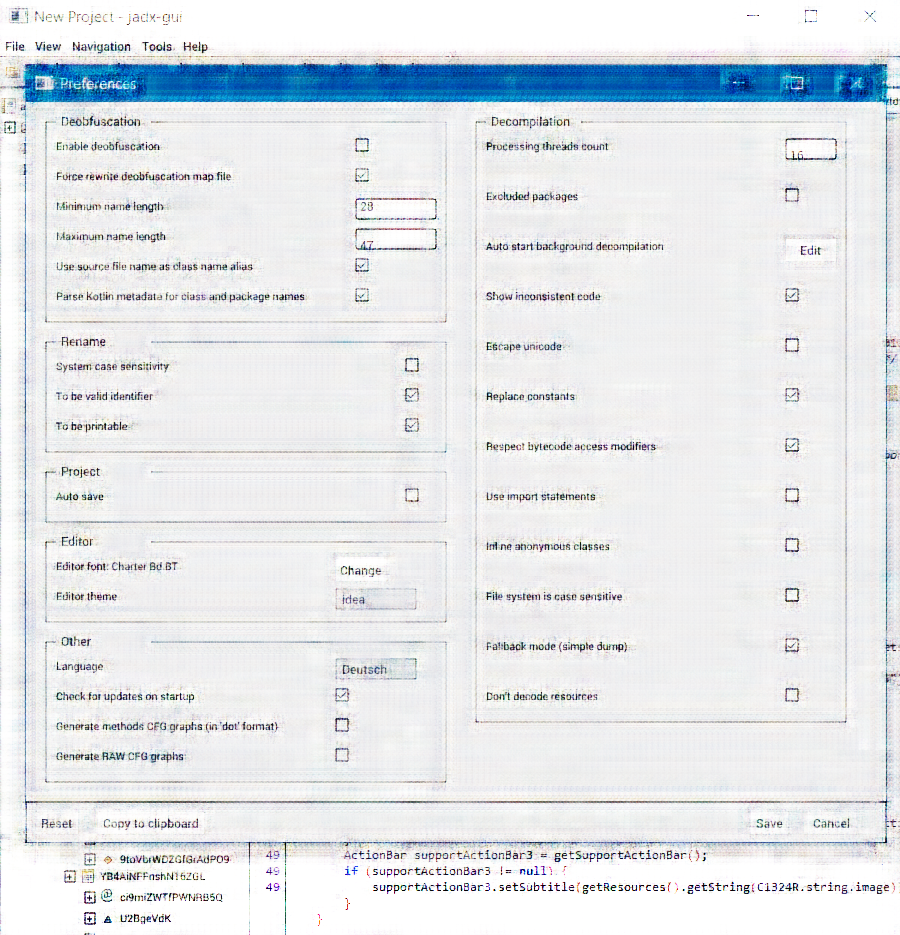
\includegraphics[width=\textwidth]{bilder/result_exp2/1_pred_a2.png}

  \caption{Experiment 2: Ausgabe des Autoencoders~\ref{a2} zu Bild 2 aus Abb.~\ref{exp2_image:2} in hoher Auflösung}
\end{figure}

\begin{figure} [ht]
  \centering
  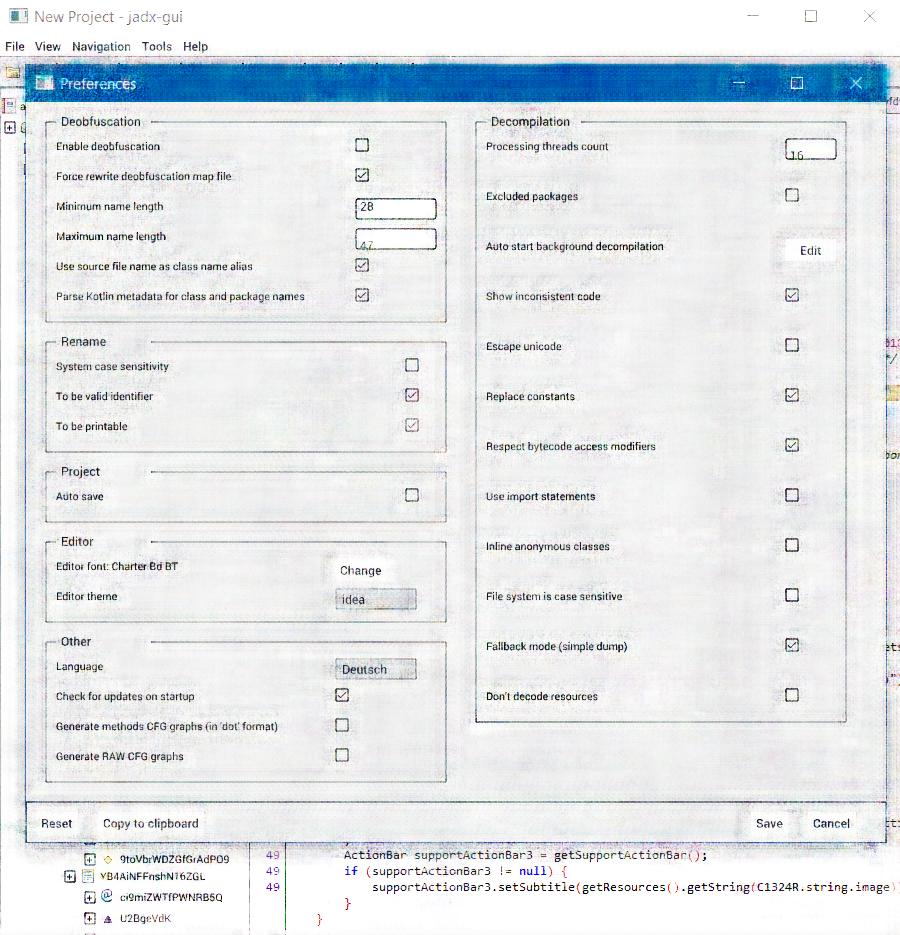
\includegraphics[width=\textwidth]{bilder/result_exp2/1_pred_a3.png}

  \caption{Experiment 2: Ausgabe des Autoencoders~\ref{a3} zu Bild 2 aus Abb.~\ref{exp2_image:2} in hoher Auflösung}
\end{figure}

\begin{figure} [ht]
  \centering
  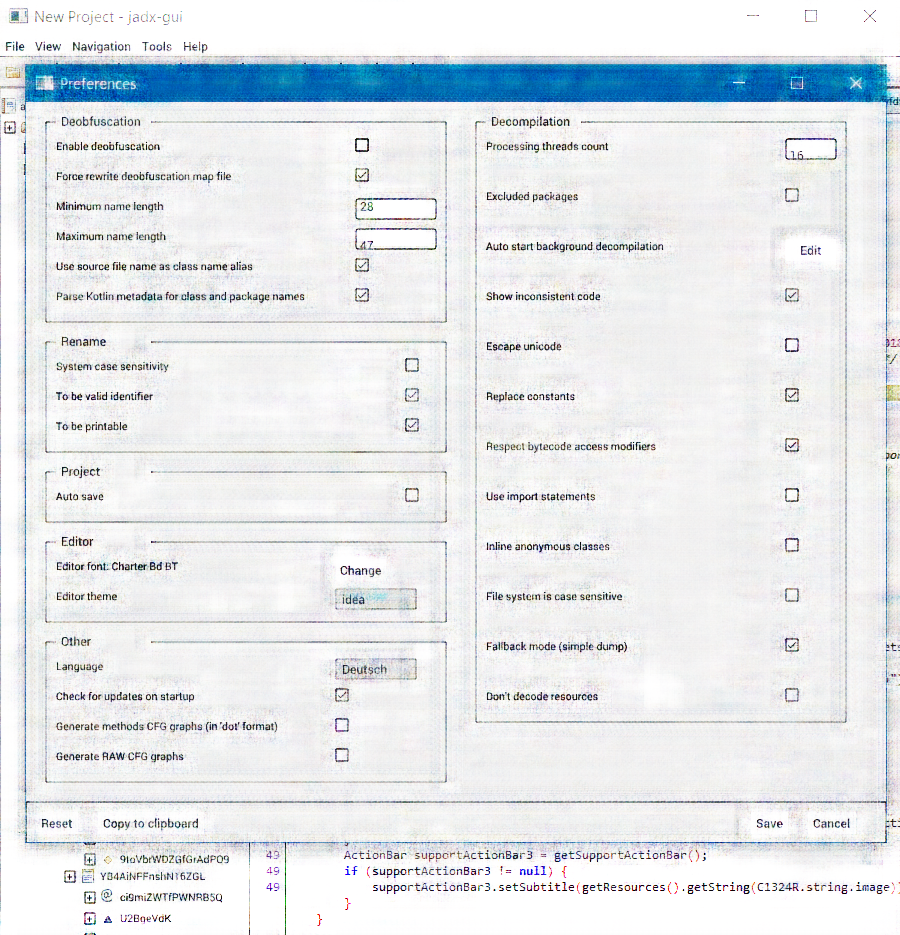
\includegraphics[width=\textwidth]{bilder/result_exp2/1_pred_a4.png}

  \caption{Experiment 2: Ausgabe des Autoencoders~\ref{a4} zu Bild 2 aus Abb.~\ref{exp2_image:2} in hoher Auflösung}
\end{figure}

\section{Resultate Experiment 3}
\label{sec:appendix:exp3}

\begin{figure} [ht]
  \centering
  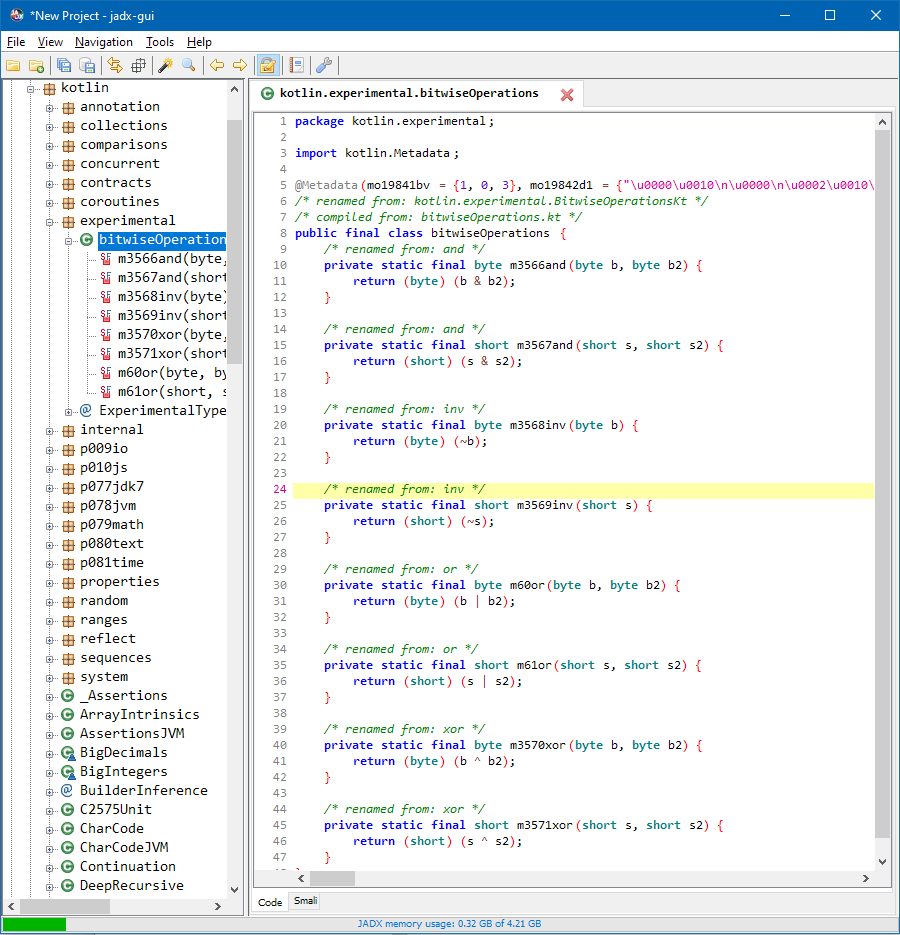
\includegraphics[width=\textwidth]{bilder/result_exp3/1.png}
  % 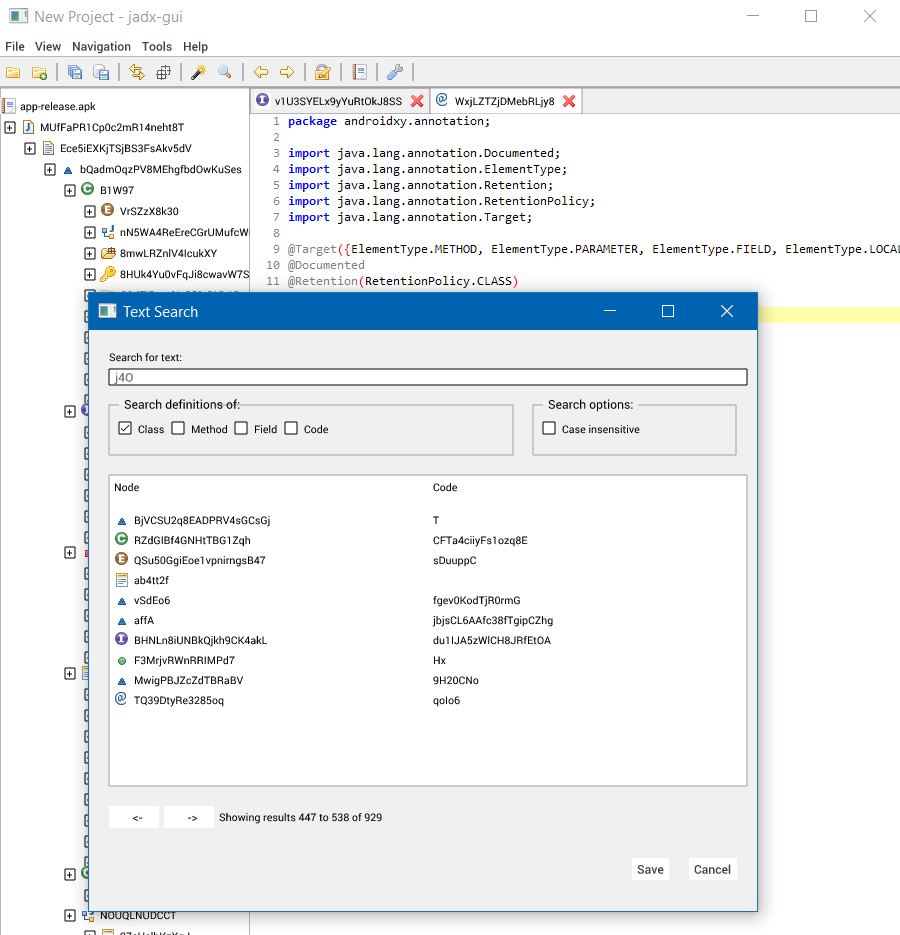
\includegraphics[width=\textwidth]{bilder/result_exp2/0.png}

  \caption{Experiment 3: Originalbild 1 aus Abb.~\ref{exp3_image:1} in hoher Auflösung}
\end{figure}

\begin{figure} [ht]
  \centering
  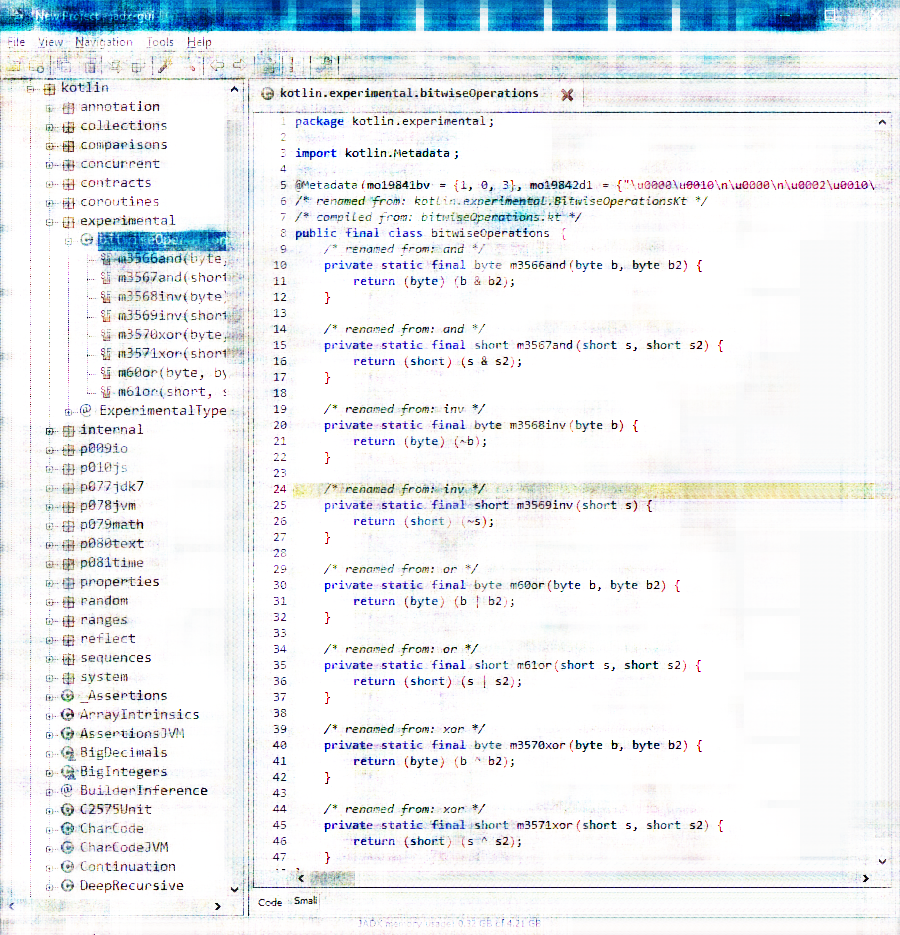
\includegraphics[width=\textwidth]{bilder/result_exp3/1_pred_a1.png}

  \caption{Experiment 3: Ausgabe des Autoencoders~\ref{a1} zu Bild 1 aus Abb.~\ref{exp3_image:1} in hoher Auflösung}
\end{figure}

\begin{figure} [ht]
  \centering
  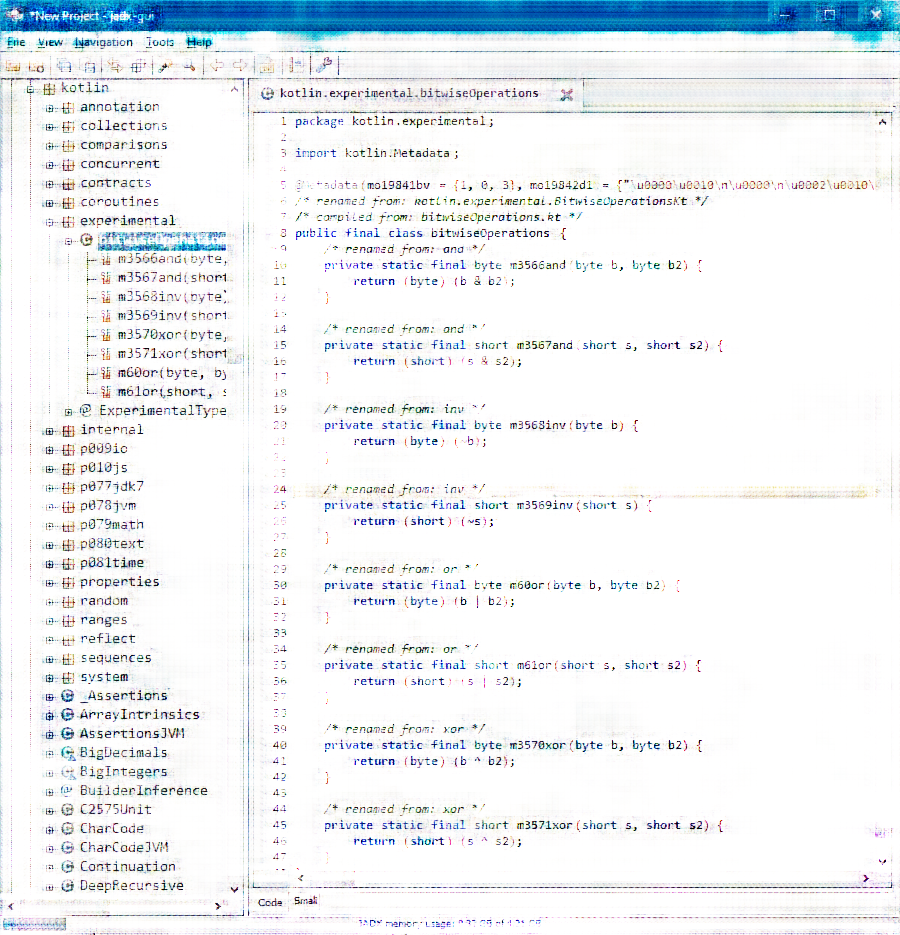
\includegraphics[width=\textwidth]{bilder/result_exp3/1_pred_a2.png}

  \caption{Experiment 3: Ausgabe des Autoencoders~\ref{a2} zu Bild 1 aus Abb.~\ref{exp3_image:1} in hoher Auflösung}
\end{figure}

\begin{figure} [ht]
  \centering
  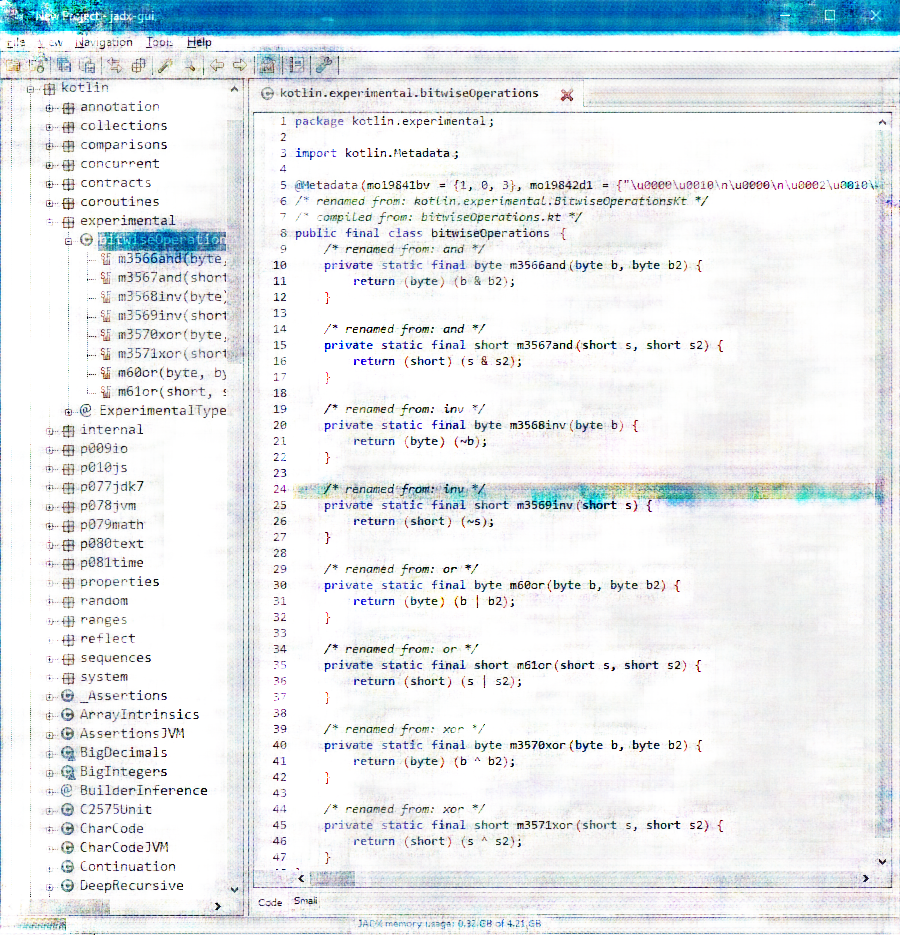
\includegraphics[width=\textwidth]{bilder/result_exp3/1_pred_a3.png}

  \caption{Experiment 3: Ausgabe des Autoencoders~\ref{a3} zu Bild 1 aus Abb.~\ref{exp3_image:1} in hoher Auflösung}
\end{figure}

\begin{figure} [ht]
  \centering
  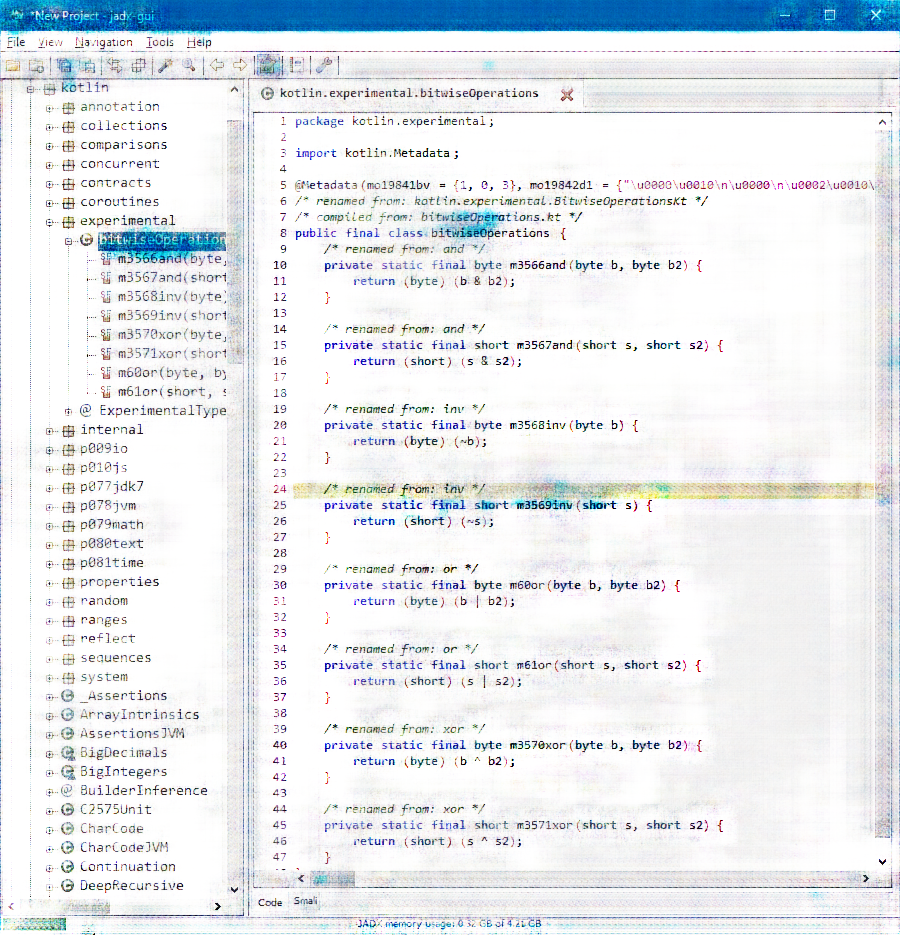
\includegraphics[width=\textwidth]{bilder/result_exp3/1_pred_a4.png}

  \caption{Experiment 3: Ausgabe des Autoencoders~\ref{a4} zu Bild 1 aus Abb.~\ref{exp3_image:1} in hoher Auflösung}
\end{figure}

\label{sec:appendix:exp3_2}
\begin{figure} [ht]
  \centering
  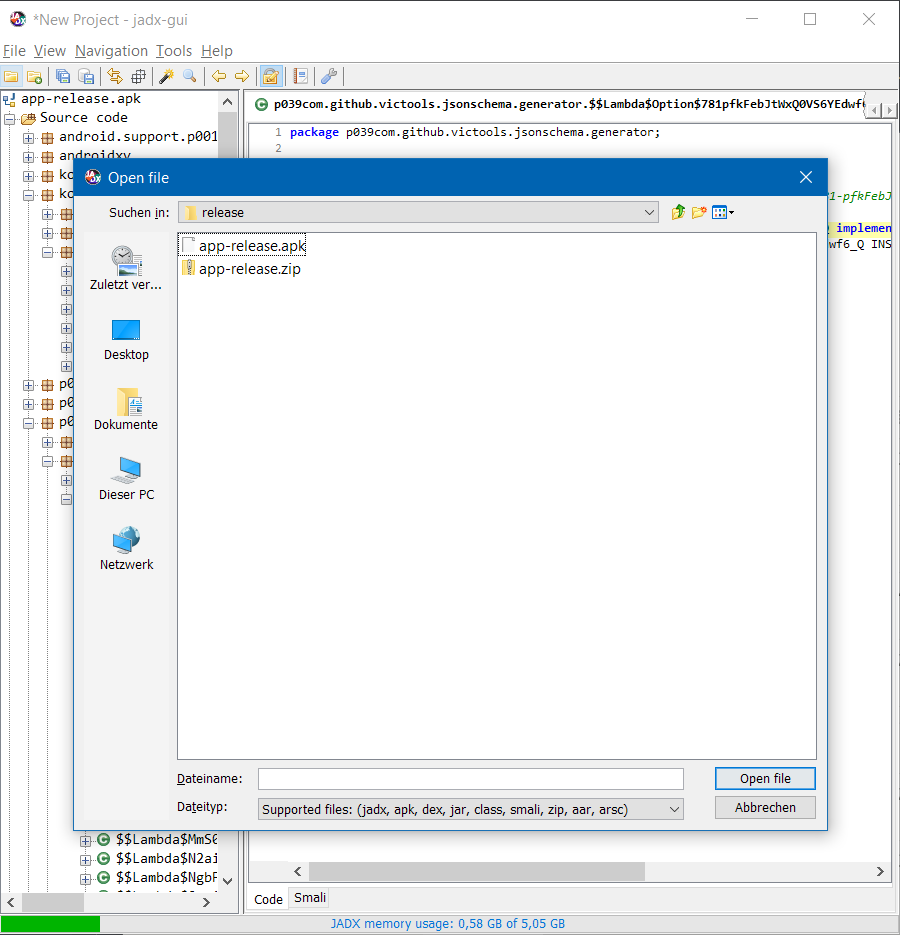
\includegraphics[width=\textwidth]{bilder/result_exp3/2.png}

  \caption{Experiment 3: Originalbild 2 aus Abb.~\ref{exp3_image:2} in hoher Auflösung}
\end{figure}

\begin{figure} [ht]
  \centering
  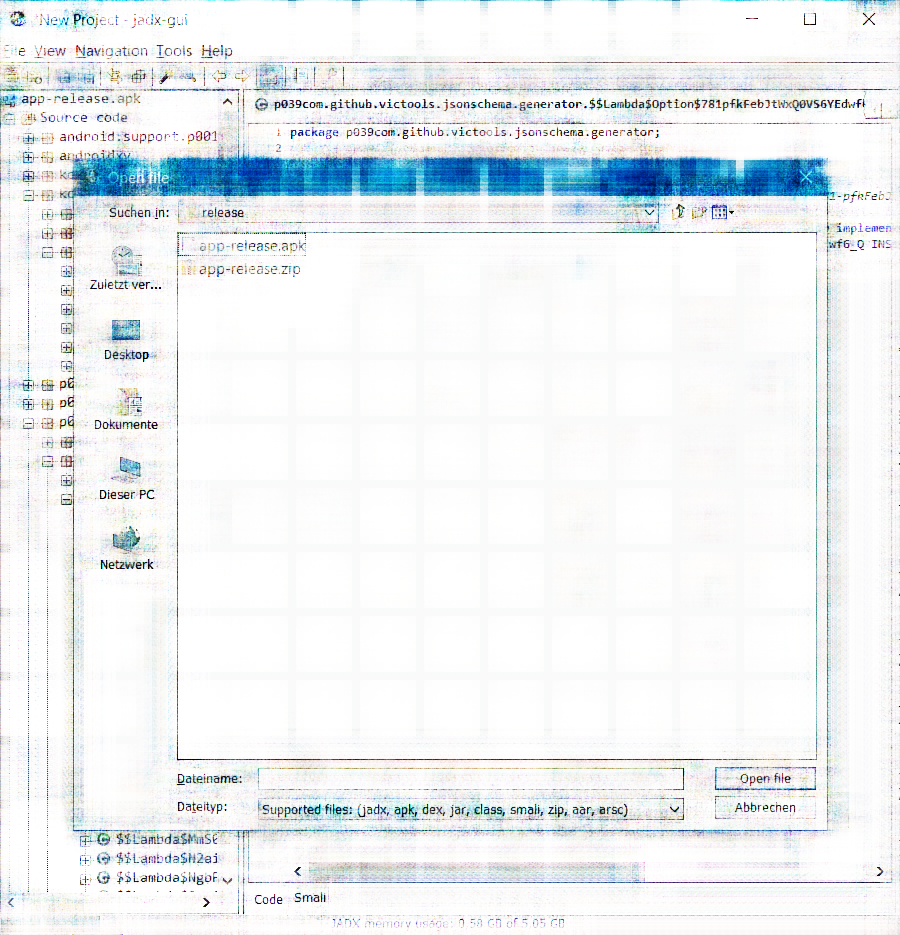
\includegraphics[width=\textwidth]{bilder/result_exp3/2_pred_a1.png}

  \caption{Experiment 3: Ausgabe des Autoencoders~\ref{a1} zu Bild 2 aus Abb.~\ref{exp3_image:2} in hoher Auflösung}
\end{figure}

\begin{figure} [ht]
  \centering
  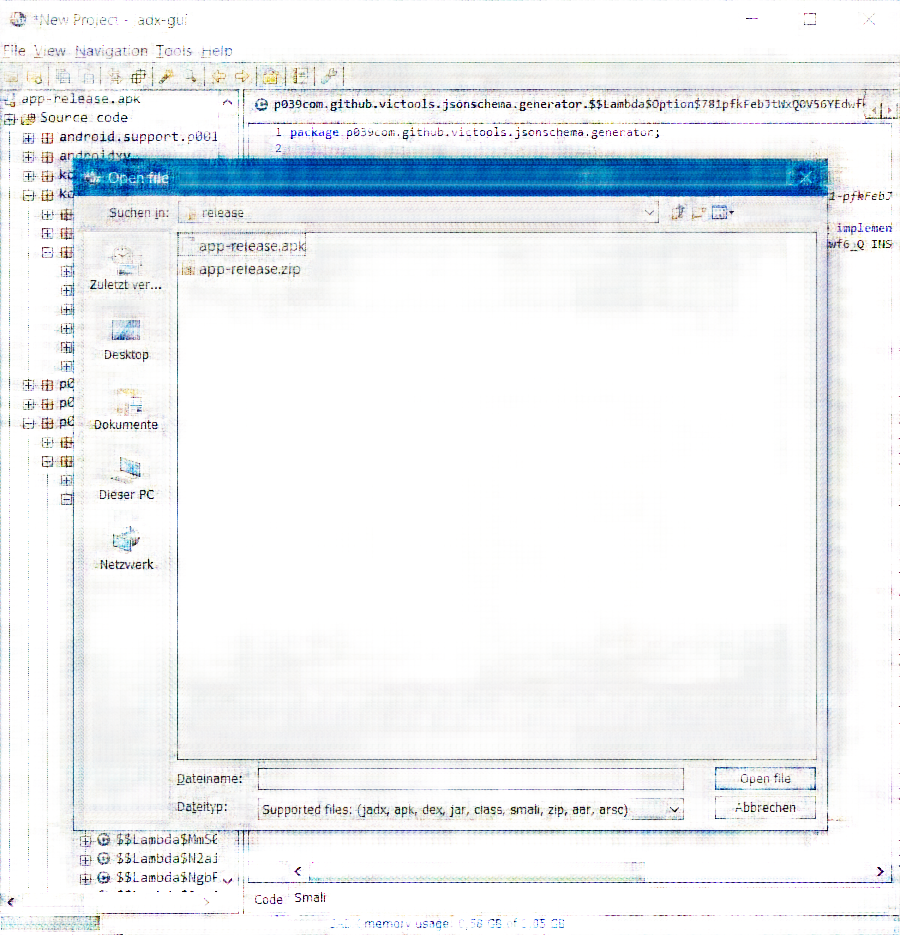
\includegraphics[width=\textwidth]{bilder/result_exp3/2_pred_a2.png}

  \caption{Experiment 3: Ausgabe des Autoencoders~\ref{a2} zu Bild 2 aus Abb.~\ref{exp3_image:2} in hoher Auflösung}
\end{figure}

\begin{figure} [ht]
  \centering
  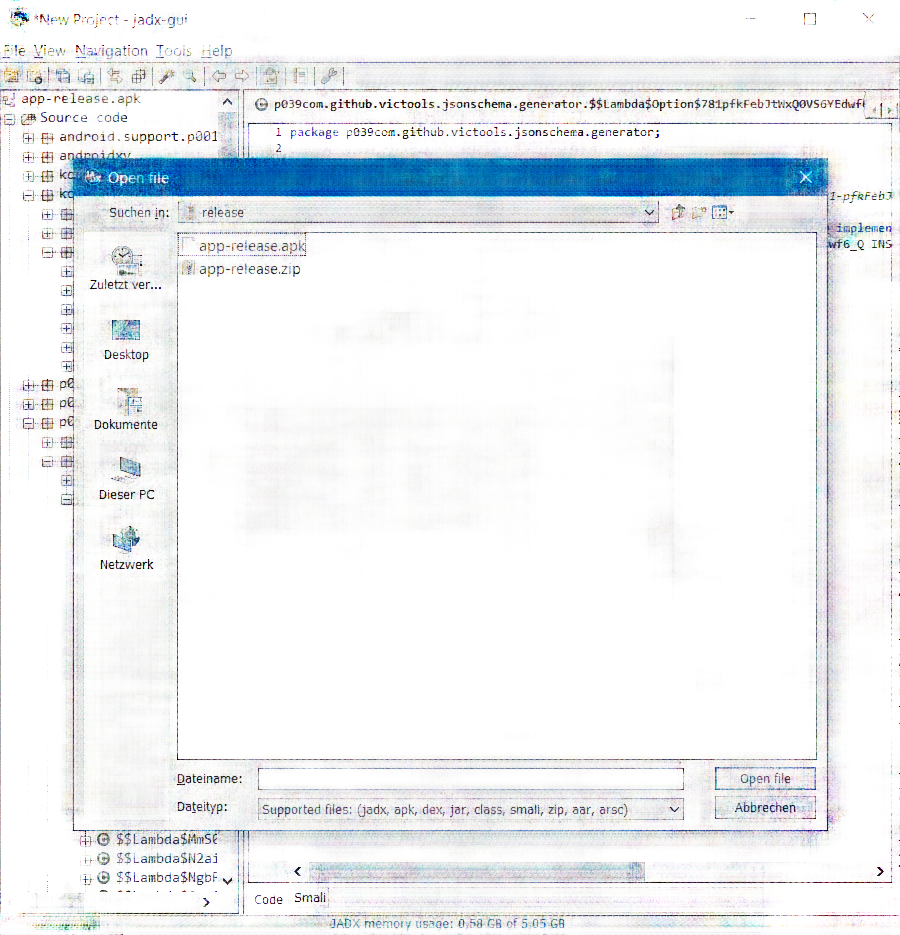
\includegraphics[width=\textwidth]{bilder/result_exp3/2_pred_a3.png}

  \caption{Experiment 3: Ausgabe des Autoencoders~\ref{a3} zu Bild 2 aus Abb.~\ref{exp3_image:2} in hoher Auflösung}
\end{figure}

\begin{figure} [ht]
  \centering
  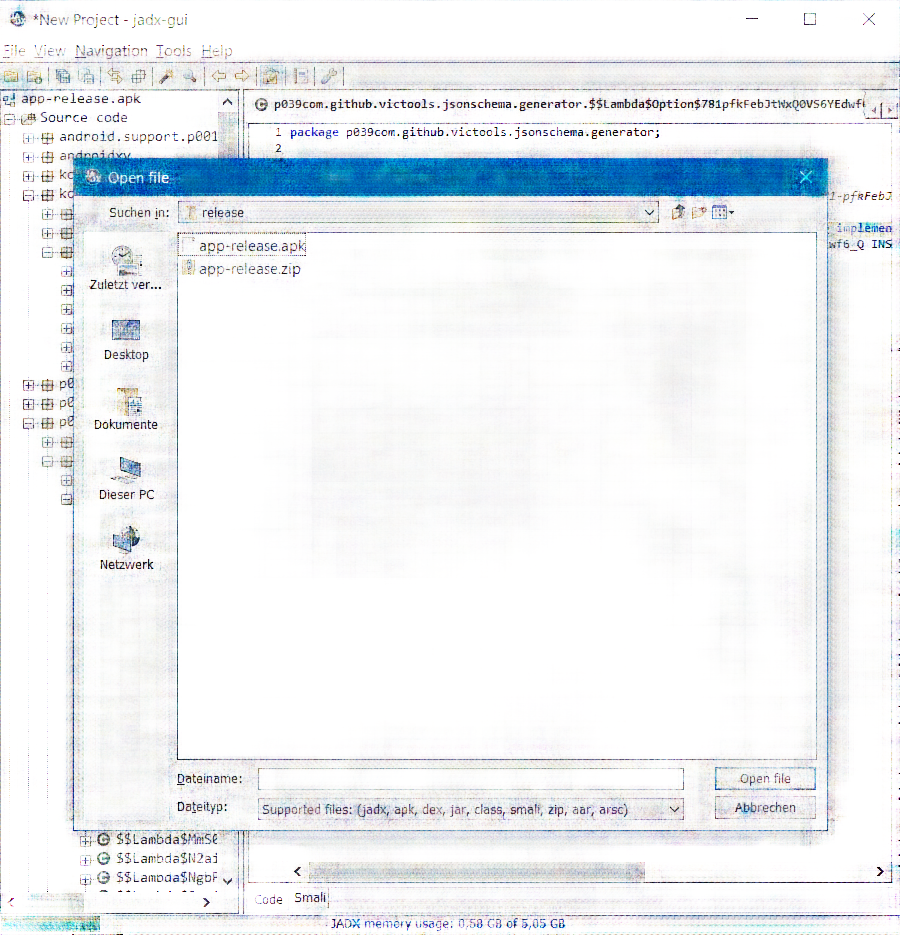
\includegraphics[width=\textwidth]{bilder/result_exp3/2_pred_a4.png}

  \caption{Experiment 3: Ausgabe des Autoencoders~\ref{a4} zu Bild 2 aus Abb.~\ref{exp3_image:2} in hoher Auflösung}
\end{figure}


\section{Resultate Experiment 4}
\label{sec:appendix:exp4}

\begin{figure} [ht]
  \centering
  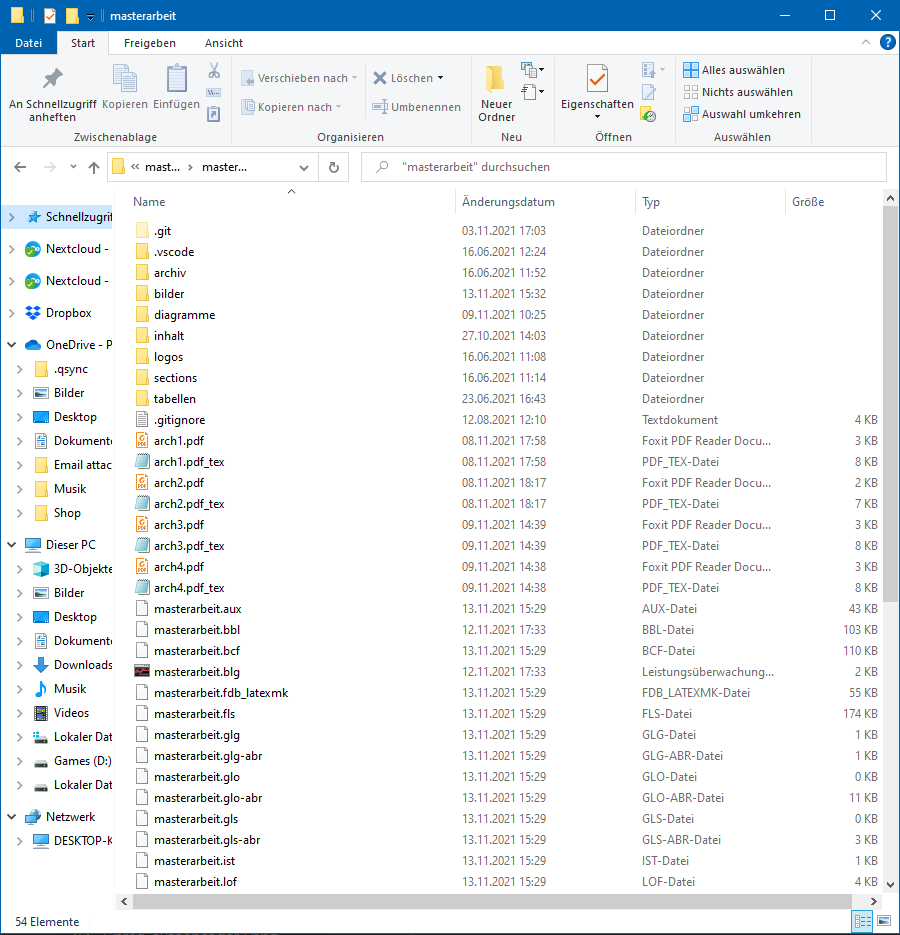
\includegraphics[width=\textwidth]{bilder/result_exp4/3.png}
  % 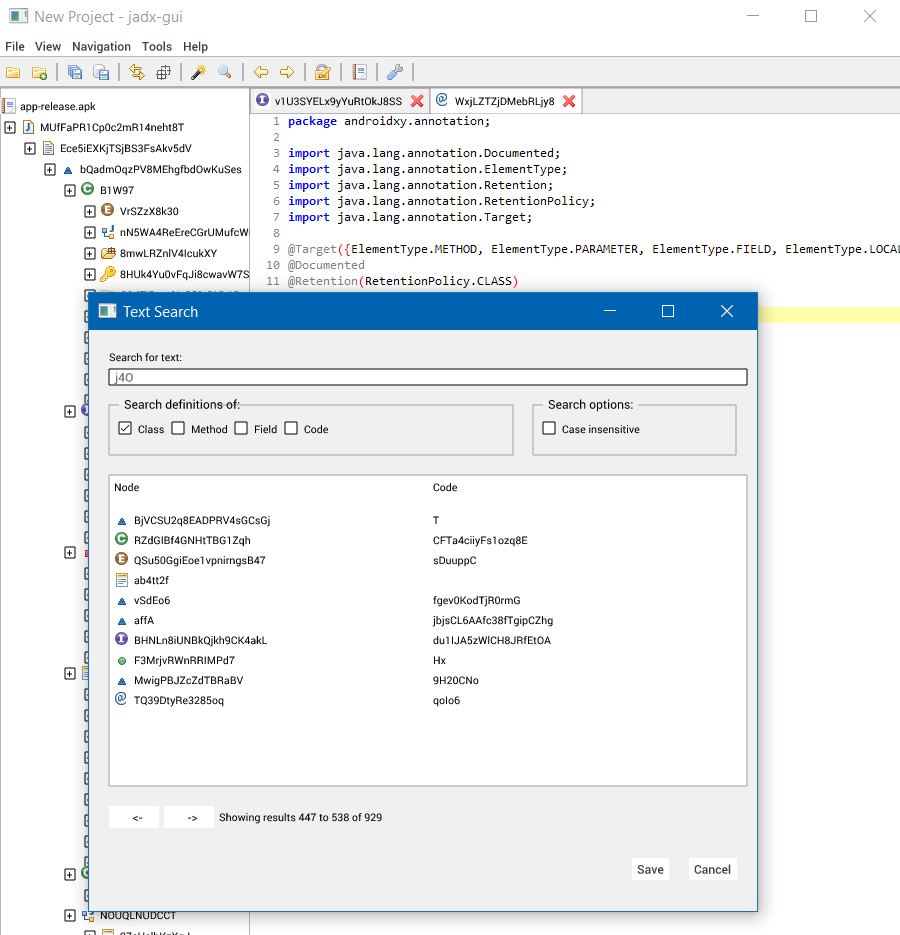
\includegraphics[width=\textwidth]{bilder/result_exp2/0.png}

  \caption{Experiment 4: Originalbild 1 aus Abb.~\ref{exp4_image:1} in hoher Auflösung}
\end{figure}

\begin{figure} [ht]
  \centering
  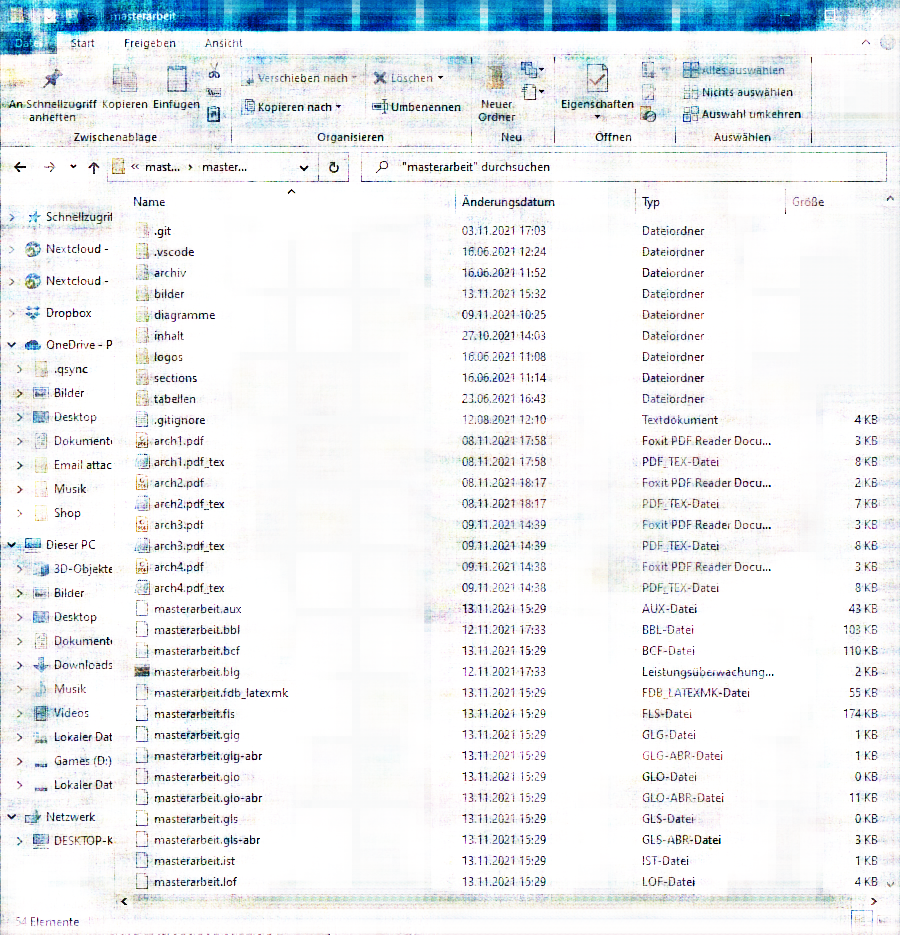
\includegraphics[width=\textwidth]{bilder/result_exp4/3_pred_a1.png}

  \caption{Experiment 4: Ausgabe des Autoencoders~\ref{a1} zu Bild 1 aus Abb.~\ref{exp4_image:1} in hoher Auflösung}
\end{figure}

\begin{figure} [ht]
  \centering
  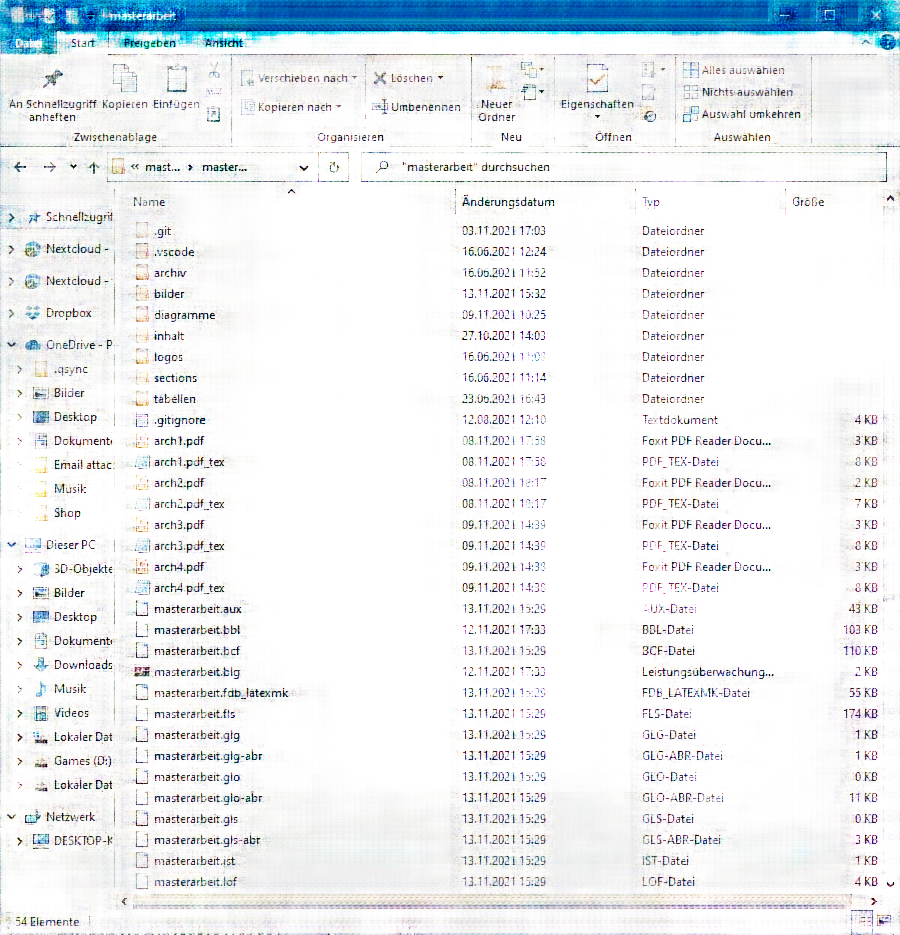
\includegraphics[width=\textwidth]{bilder/result_exp4/3_pred_a2.png}

  \caption{Experiment 4: Ausgabe des Autoencoders~\ref{a2} zu Bild 1 aus Abb.~\ref{exp4_image:1} in hoher Auflösung}
\end{figure}

\begin{figure} [ht]
  \centering
  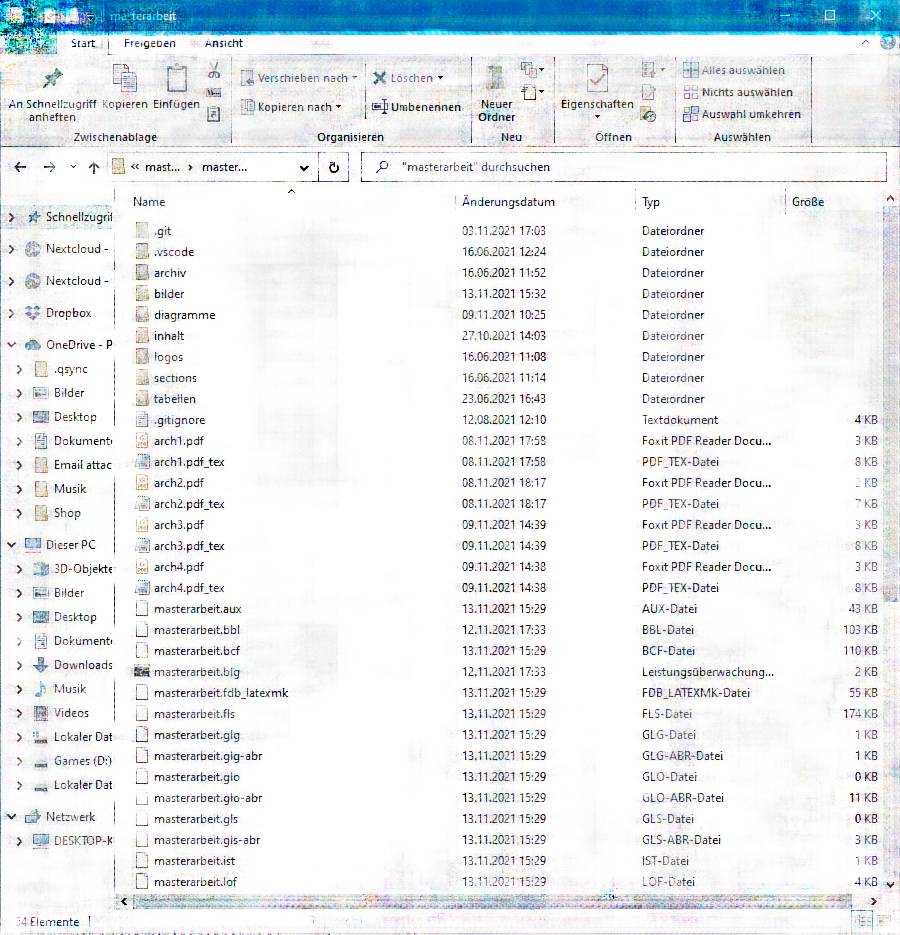
\includegraphics[width=\textwidth]{bilder/result_exp4/3_pred_a3.png}

  \caption{Experiment 4: Ausgabe des Autoencoders~\ref{a3} zu Bild 1 aus Abb.~\ref{exp4_image:1} in hoher Auflösung}
\end{figure}

\begin{figure} [ht]
  \centering
  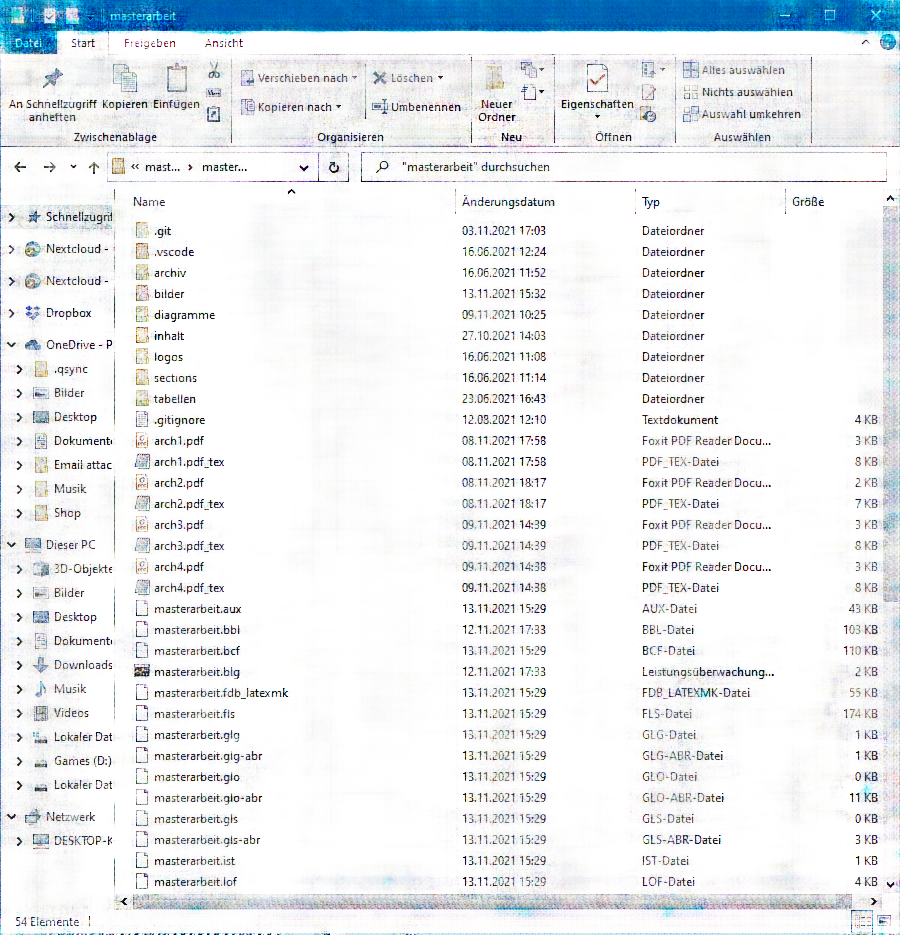
\includegraphics[width=\textwidth]{bilder/result_exp4/3_pred_a4.png}

  \caption{Experiment 4: Ausgabe des Autoencoders~\ref{a4} zu Bild 1 aus Abb.~\ref{exp4_image:1} in hoher Auflösung}
\end{figure}

\label{sec:appendix:exp4_2}
\begin{figure} [ht]
  \centering
  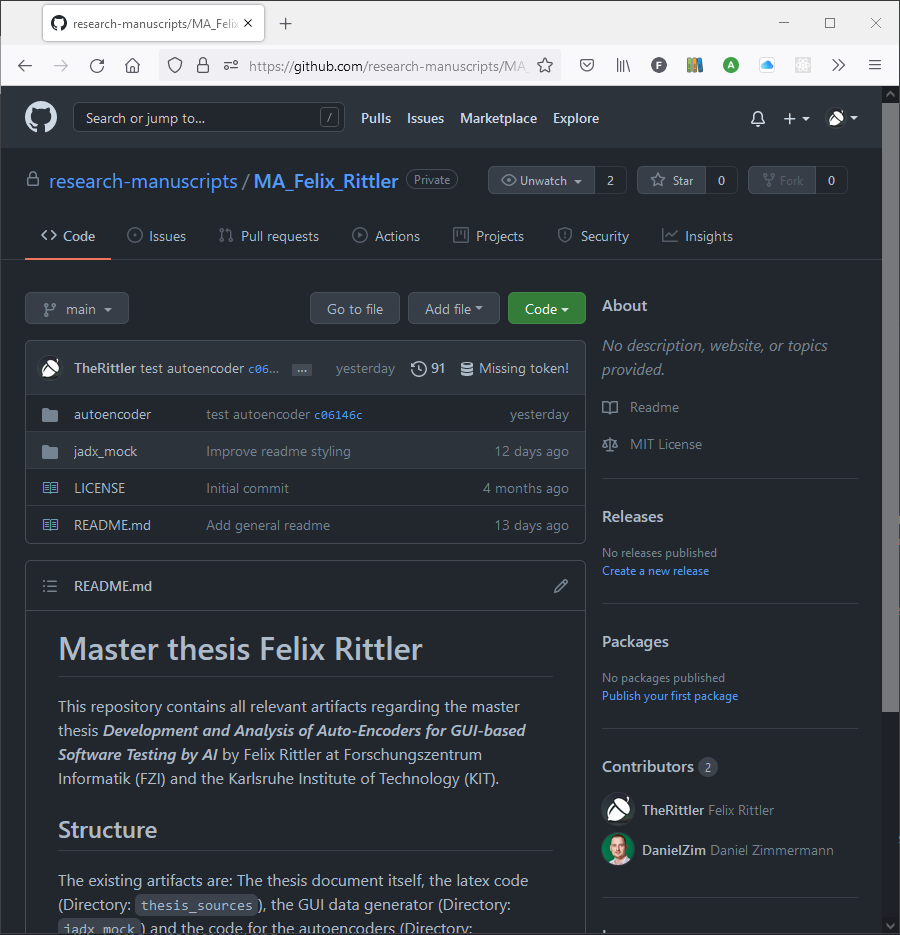
\includegraphics[width=\textwidth]{bilder/result_exp4/4.png}

  \caption{Experiment 4: Originalbild 2 aus Abb.~\ref{exp4_image:2} in hoher Auflösung}
\end{figure}

\begin{figure} [ht]
  \centering
  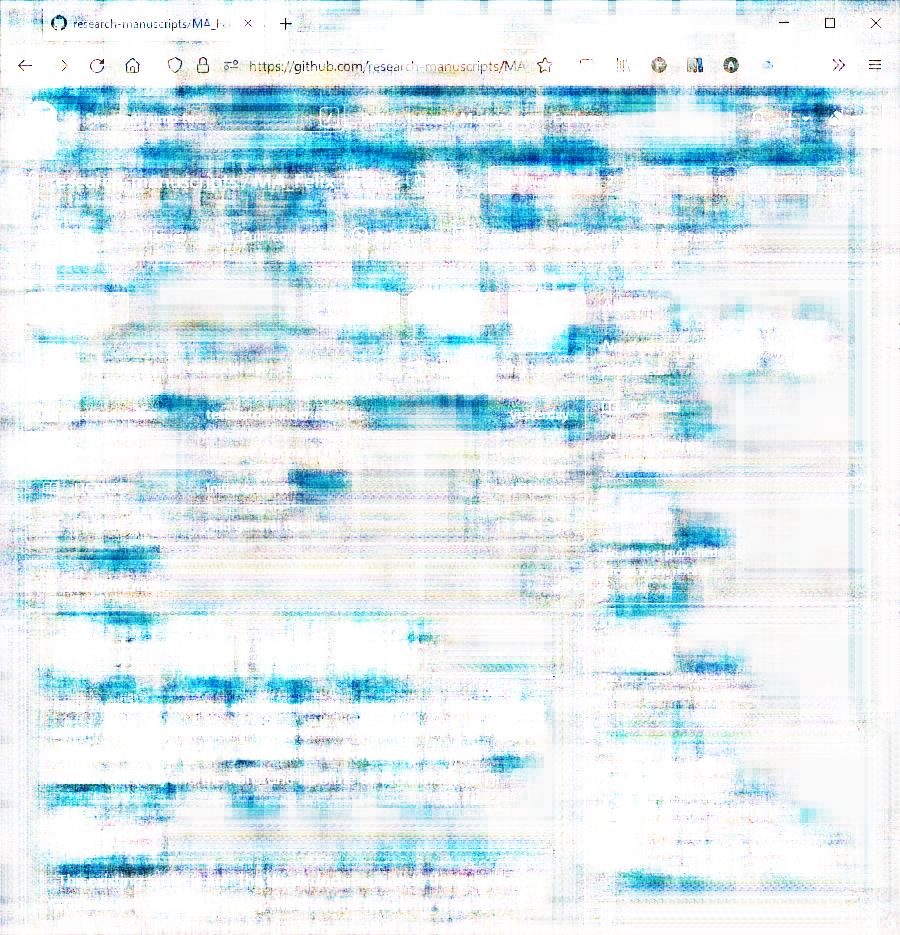
\includegraphics[width=\textwidth]{bilder/result_exp4/4_pred_a1.png}

  \caption{Experiment 4: Ausgabe des Autoencoders~\ref{a1} zu Bild 2 aus Abb.~\ref{exp4_image:2} in hoher Auflösung}
\end{figure}

\begin{figure} [ht]
  \centering
  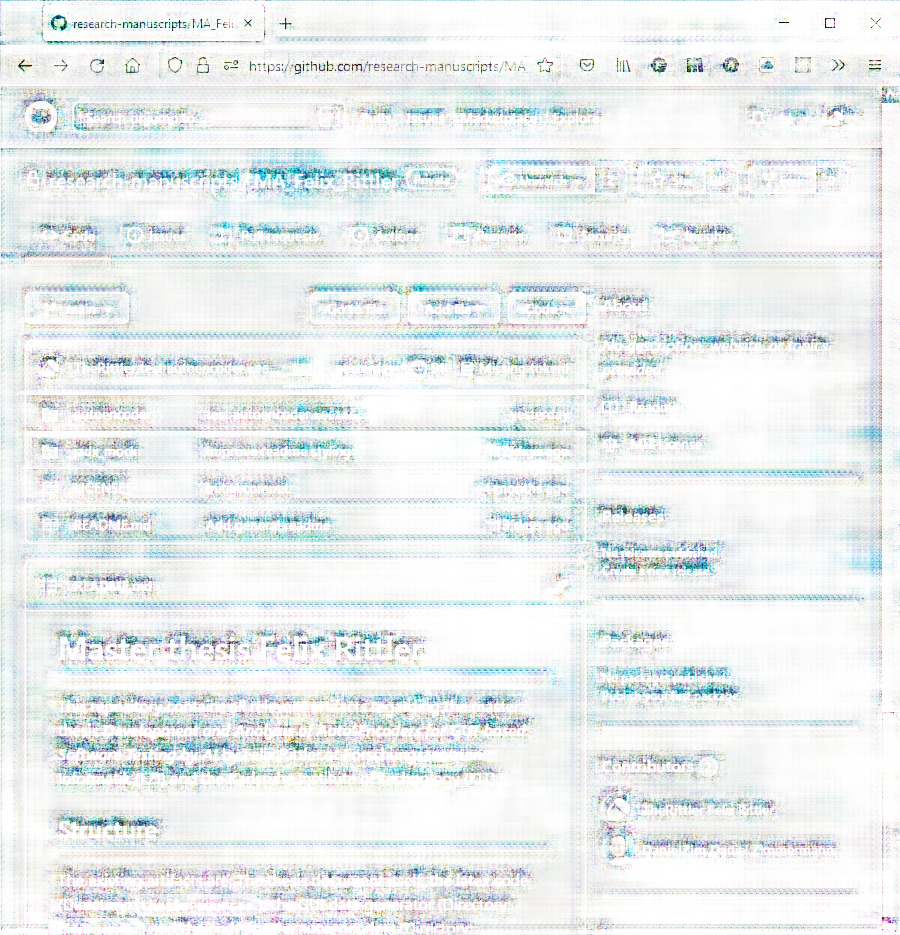
\includegraphics[width=\textwidth]{bilder/result_exp4/4_pred_a2.png}

  \caption{Experiment 4: Ausgabe des Autoencoders~\ref{a2} zu Bild 2 aus Abb.~\ref{exp4_image:2} in hoher Auflösung}
\end{figure}

\begin{figure} [ht]
  \centering
  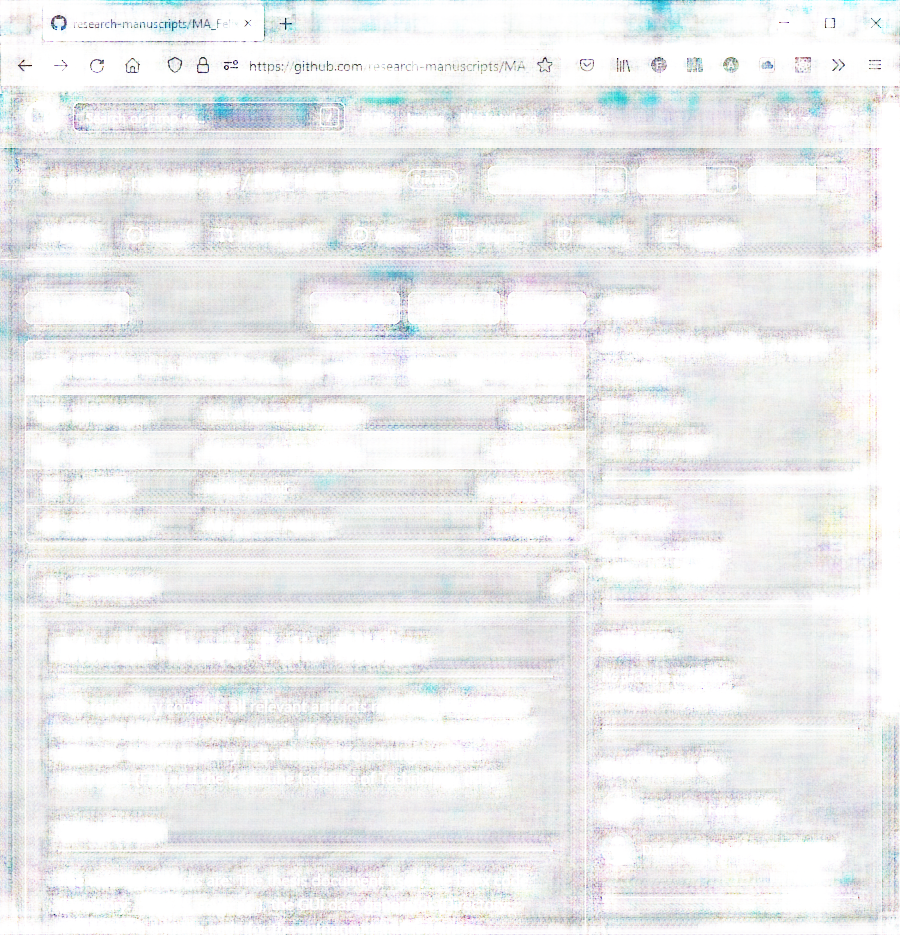
\includegraphics[width=\textwidth]{bilder/result_exp4/4_pred_a3.png}

  \caption{Experiment 4: Ausgabe des Autoencoders~\ref{a3} zu Bild 2 aus Abb.~\ref{exp4_image:2} in hoher Auflösung}
\end{figure}

\begin{figure} [ht]
  \centering
  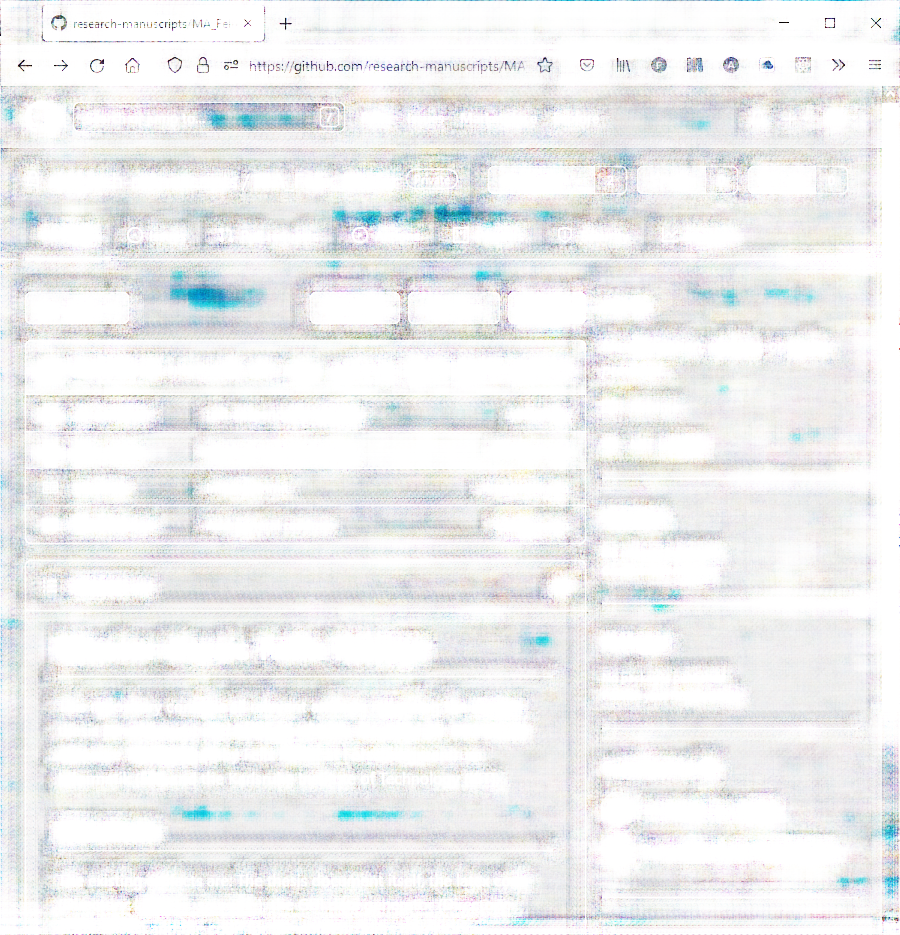
\includegraphics[width=\textwidth]{bilder/result_exp4/4_pred_a4.png}

  \caption{Experiment 4: Ausgabe des Autoencoders~\ref{a4} zu Bild 2 aus Abb.~\ref{exp4_image:2} in hoher Auflösung}
\end{figure}

\setcounter{figure}{0}

% \begin{figure} [ht]
%   \centering
%   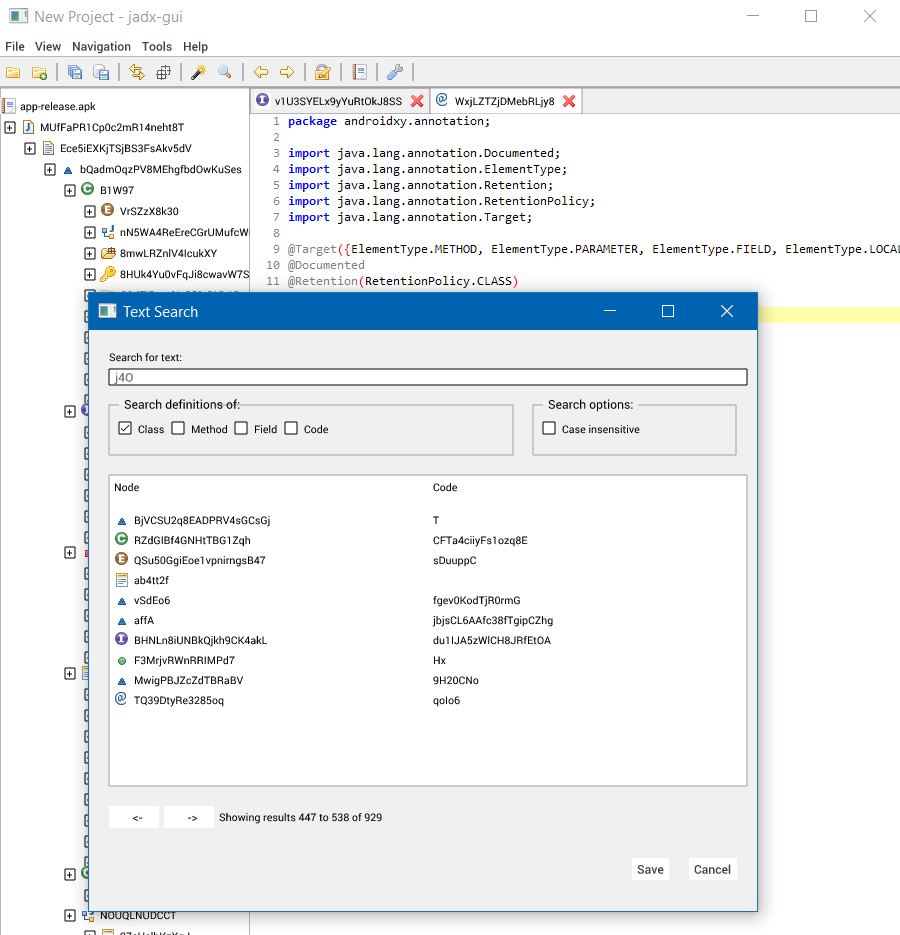
\includegraphics{bilder/result_exp2/0.png}
%   \caption{A figure}
% \end{figure}


%% ---------------------
%% | / Example content |
%% ---------------------

\end{document}
